\documentclass[british,titlepage,oneside]{ntnuthesis}

%\usepackage{todonotes}
\usepackage{tabularx}
%\usepackage{tikz-timing}
%\usepackage{tikz-timing}[2009/05/15]
\usepackage{tikz-timing}[2017/12/20]
\usepackage{tikz}
%\usetikzlibrary{matrix}
%\usepackage{paralist}
%\usepackage{subfig}

\usepackage{svg}

\usepackage{pgfgantt}
\definecolor{blue}{HTML}{74BBC9}
\definecolor{yellow}{HTML}{F7E967}

\newcommand{\sv}[1]{\lstinline{#1}} %systemverilog code
\newcommand{\rv}[1]{\lstinline{#1}} %riscv instructions, csrs etc
\newcommand{\ccode}[1]{\lstinline{#1}} %c code
\newcommand{\file}[1]{\lstinline{#1}}
\newcommand{\dir}[1]{\lstinline{#1}}

\newcommand{\tmp}[1]{\textcolor{red}{#1}}

\newenvironment{svblock}[1][]
    {\begin{lstlisting}[#1]}
    {\end{lstlisting}}

\lstnewenvironment{systemverilog}[1][]
{\lstset{language=verilog,
        #1
        }}
{}

\lstnewenvironment{clisting}[1][]
{\lstset{language=c,
        #1
        }}
{}

\lstnewenvironment{terminal}[1][]
{\lstset{language=c,
        #1
        }}
{}
%\begin{lstlisting}[label={lst:async_int_1},caption={Trace output from asynchronous interrupts without pipeline shell}]

\crefname{rmReq}{RM Requirement}{RM Requirements}
\crefname{psReq}{PS Requirement}{PS Requirements}
\crefname{issReq}{ISS Requirement}{ISS Requirements}

\title{Designing a RISC-V Reference Model for Open Source Processor Cores}
\shorttitle{RISC-V Reference Model}
\author{Torje Nygaard Eikenes}
\shortauthor{Torje N. Eikenes}
\date{\today}

%\addbibresource{thesis.bib}
%\addbibresource{bib/Formal.bib}
\addbibresource{bib/MyLibrary.bib}


% From https://www.overleaf.com/learn/latex/Glossaries

\makeglossaries % Prepare for adding glossary entries


\newglossaryentry{ps}
{
    name=Pipeline Shell,
    description=Shell responsible for the cycle-accurate timing of the values generated by the \acrshort{iss}
}

\newglossaryentry{stagebased}
{
    name=stage-based pipeline simulation,
    description=
}

\newglossaryentry{timewheel}
{
    name=Cycle-based time wheel simulation,
    description=
}

\newglossaryentry{cv32s}
{
    name=CV32E40S,
    description=An open source RISC-V processor from the OpenHW Group.
}

\newglossaryentry{cv32x}
{
    name=CV32E40X,
    description=An open source RISC-V processor from the OpenHW Group.
}

\newglossaryentry{core-v-verif}
{
    name=core-v-verif,
    description=An open source RISC-V processor from the OpenHW Group.
}


\newglossaryentry{flush}
{
    name=Flush,
    description=To clear uncommited instructions from the pipeline. 
}

\newglossaryentry{commited}
{
    name=Commited,
    description=When the results of an instruction is written back to the register file in the Writeback stage of the pipeline.
}

\newglossaryentry{retired}
{
    name=Retired,
    description=When an instruction is \gls{commited} after being in the WB stage and is no longer in the pipeline.
}

% --------------------
% ----- Acronyms -----
% --------------------

\newacronym{riscv}{RISC-V}{Reduced Instruction Set Computer (RISC) Five}
\newacronym{iss}{ISS}{Instruction Set Simulator}
\newacronym{dut}{DUT}{Device Under Test}
\newacronym{fev}{FEV}{Formal Equivalence Verification}
\newacronym{rtl}{RTL}{Register Transfer Level}
\newacronym{isa}{ISA}{Instruction Set Architecture}
\newacronym{rm}{RM}{Reference Model}
\newacronym{sva}{SVA}{SystemVerilog Assertions}
\newacronym{fv}{FV}{Formal Verification}
\newacronym{rvfi}{RVFI}{RISC-V Formal Interface}
\newacronym{bsp}{BSP}{Board Support Package}
\newacronym{if}{IF}{Instruction Fetch}
\newacronym{id}{ID}{Instruction Decode}
\newacronym{ex}{EX}{Execute}
\newacronym{wb}{WB}{Write-back}
\newacronym{lsu}{LSU}{Load Store Unit}
\newacronym{csr}{CSR}{Control and Status Register}


 % add glossary and acronym lists before document

\begin{document}

\chapter*{Abstract}

Asynchronous events like interrupts and debug requests pose a significant challenge in processor verification, often leading to elusive bugs. 
\textit{Instruction Set Simulators (ISS)} are often used as a Reference Model to verify the correctness of a processor's execution and are often sufficient in normal execution. 
However, due to their instruction-level abstraction level, ISSs can not accurately simulate the timing of asynchronous events and side effects compared to the processor core. Therefore, a more advanced Reference Model that accurately simulates the timing and correctness of asynchronous events is needed.


This thesis explores and compares different approaches to implementing a reference model for open-source RISC-V processor cores that can accurately simulate asynchronous events at the cycle level. We propose a reference model architecture combining a "Pipeline Shell" and an existing ISS. The pipeline shell is responsible for modeling the timing of the pipeline and the behavior of asynchronous events, while the ISS is responsible for the functional execution of the instructions. The reference model is implemented in SystemVerilog and integrated into the OpenHW Group's verification environment for the CV32E40S core by Silicon Labs. We also focus on making the reference model compatible with formal verification.

The results show that the reference model can correctly simulate asynchronous events in many different scenarios. It has a smaller verification gap compared to using a traditional ISS as a reference model and is likely to find bugs that other reference model solutions can not. The ISS used is not compatible with formal verification. Still, the rest of the design is believed to be compatible with formal verification if the ISS is replaced with a synthesizable ISS. However, the current implementation has some limitations. The reference model is currently dependent on the DUT core for some pipeline timing details, and the complexity of the pipeline shell has led to multiple unresolved bugs.








\chapter*{Sammendrag}

Nøye verifikasjon er avgjørende ved utviklig av prosessorkjerner og tar en betydelig del av den totale utviklingstiden.
Asynkrone hendelser som "interrupts" er en stor utfordring i prosessorverifisering, som ofte fører til vanskelige feil. \textit{InstruksjonssettSimulatorer} (ISS) brukes ofte som referansemodell for å verifisere prosessorkjerner, og er ofte tilstrekkelig for normal gjennomkjøring av prosessoren. På grunn av deres høye abstraksjonsnivå kan imidlertid ikke ISS-er nøyaktig simulere timingen og virkningen av asynkrone hendelser på samme måte som en prosessor\-kjerne. Det er derfor behov for en mer avansert referansemodell som nøyaktig simulerer timingen og korrekt\-heten av asynkrone hendelser. 

I denne masteroppgaven utforsker og sammenligner vi ulike tilnærminger til implementeringen av en referansemodell for åpne RISC-V prosessorkjerner som kan simulere asynkrone hendelser på syklusnivå.  Vi foreslår og implementerer en referansemodellarkitektur som kombinerer et “Pipeline-Skall” og en eksisterende ISS. Pipeline-skallet er ansvarlig for å modellere timingen til pipelinen og asynkrone hendelser, mens ISSen er ansvarlig for den funksjonelle utførelsen av instruksjonene. Referansemodellen er implementert i SystemVerilog og integrert i OpenHW Groups verifiseringsmiljø for CV32E40S-kjernen til Silicon Labs. Spike er valgt som den eksisterende ISSen, og de nødvendige modifikajonene blir diskutert. I tillegg fokuserer vi på å gjøre referansemodellen kompatibel med formell verifisering.

Resultatene viser at referansemodellen kan simulere asynkrone hendelser korrekt i mange ulike scenarier. Den har et mindre verifikasjonsgap sammenlignet med å bruke en tradisjonell ISS som referansemodell, og kan sannsynligvis finne feil som andre referansemodelløsninger ikke kan. ISSen som brukes er ikke kompatibel med formell verifikasjon, men resten av designet antas å være kompatibelt med formell verifikasjon dersom ISSen erstattes med en syntetiserbar ISS. Imidlertid har de nåværende implementeringen noen begrensninger. Den implementerte referansemodellen er avhengig av signaler fra prosessorkjernen for noen detaljer i pipelinetimingen, og kompleksiteten til pipeline-skallet har ført til flere hittil uløste feil.



\chapter*{Preface}


\section{Previous work}

Before this thesis, the author wrote a specialization project report \cite{torjenygaardeikenesDesigningRISCVReference2023}. The chapters and sections listed below have been reused with varying resemblance to \cite{torjenygaardeikenesDesigningRISCVReference2023}. The findings from the report will be presented in \cref{sec:specialization}.


\begin{enumerate}
    \item \textbf{Introduction} \cref{Introduction} is based on the same chapter in \cite{torjenygaardeikenesDesigningRISCVReference2023}.
    \item \textbf{Background} \cref{sec:bg_pipeline} to \cref{sec:bg_cycle-accurate} is based on the same sections from \cite{torjenygaardeikenesDesigningRISCVReference2023}.
    \item \textbf{Previous work} The relevant findings from the report will be described in \cref{sec:specialization}.
\end{enumerate}





%
%
%result of the course \textit{TFE4580 - Electronic Systems Design and Innovation, Specialization Project} at the Norwegian University of Science and Technology (NTNU). Silicon Laboratories Norway AS gave the project
%
%I would like to thank my supervisors Per Gunnar Kjeldsberg from NTNU, and Marton Teilgård from Silicon Laboratories Norway AS, for their guidance throughout the project.
%

\section{Acknowledgments}





\tableofcontents
\listoffigures
\listoftables
\lstlistoflistings

\printglossary[type=\acronymtype] % Print acronyms
\printglossary                    % Print glossary


\chapter{Introduction and motivation}
\label{Introduction} 

%1. Establishing your research territory
%2. Constructing the research gap or niche
%3. Pointing out the gap/niche
%4. Stating your purpose. Aim statement or research question
%5. Highlighting benefits and mapping out the paper


%1. Statements about the field of research
%to provide the reader with a setting or
%context for the problem to be
%investigated and claimed its centrality
%or importance.
%2. More specific statements about
%the aspects of the problem already
%studied by other researchers, laying
%a foundation of information already
%known.
%3. Statements that indicate the need for
%more investigation, creating a gap or
%research niche for the present study
%to fill.
%4. Statements giving the purpose/
%objectives of the writer's study or
%outlining its main activity or findings.
%5. Optional statement(s) that provide a
%positive value or justification for
%carrying out the study.

%\section{RISC-V and Open-source processors}

\section{Motivation}


With the end of Dennard scaling and the recent slowdown of Moore's Law, achieving performance and energy efficiency improvements from scaling down the transistors is getting exponentially harder \cite{hennessyComputerArchitectureQuantitative2019}. This has led to a shift from general-purpose processor cores to \acrfull{dsa}. Companies need to specialize their processors to achieve higher performance and lower energy instead of using an available general-purpose processor \cite{mezgerSurveyRISCVArchitecture2022}. 


The growing demand for specialized processors has also led to a demand for an open and modular \textit{Instruction Set Architecture (ISA)}. The RISC-V ISA \cite{watermanRISCVInstructionSet2019,watermanRISCVInstructionSet2021}, originally developed at UC Berkeley in 2010 \cite{pattersonComputerOrganizationDesign2021}, has recently gained popularity in academia and industry because of its open-source nature, proven RISC-style, and modularity \cite{theshdgroupRISCVMarketReport2024, asanovicInstructionSetsShould2014}.
The 2024 RISC-V Market Report by \textcite{theshdgroupRISCVMarketReport2024} reports 1.3B RISC-V units shipped in 2023 and forecasts growth to 16.2B units by 2030.


The ISA consists of a base architecture with the possibility to add functionality through various standard or custom extensions\cite{watermanRISCVInstructionSet2019}. This flexibility is particularly useful for \acrshort{dsa}s. It allows designers to start with a minimal processor, extend it with only the required extensions, and possibly add custom implementation-specific instructions. Custom extensions enable compute-intensive tasks to be implemented in hardware and accessed through custom instructions. 

Being an open-source ISA, anyone can use and modify RISC-V without a licensing fee. This allows a low barrier to entry and collaboration between developers and researchers. The open nature of RISC-V open-source ISA has also led to an increasingly large ecosystem of open-source processors. One such example is the CV32E40S \cite{openhwgroupCv32e40s2024}, a processor core from the CORE-V family of processor cores from the OpenHW Group, a global organization of many companies working together to make open-source cores, tools, and software \cite{taylorAdvancedRISCVVerification2023}. The CV32E40S is a relatively small and efficient processor with a 4-stage pipeline. The core can be configured to support different RISC-V extensions and also adds the custom Xsecure extension, adding multiple security features \cite{openhwgroupIntroductionCOREVCV32E40S2023}. This processor will be used as an example throughout the report.





\subsection{Processor verification \& the need for a reference model}

Compared to trusted commercial solutions, the biggest barrier to adopting open-source processor IPs in a System-on-Chip (SoC) is the core's quality, particularly the verification effort invested in the core. Compared to open-source software, hardware typically has a much higher manufacturing cost, increasing the verification requirements \cite{kevinmcdermottOpenHWIndustrialGradeVerification2022}.
With RISC-V, where "anyone" can make a processor, the verification responsibility is now moved from a few specialized IP suppliers to every SoC developer. 

Therefore, a versatile and open verification environment is essential to RISC-V's continuing popularity and growth. Verification is a crucial aspect of processor development, consuming a significant portion of the overall development time. If every developer team were to build their verification environment from scratch, the adoption of RISC-V would likely stagnate.

Conventional manual testing with predetermined outcomes can be time-consuming and inadequate to thoroughly validate a processor's complex behavior. Instead, constrained random testing is often used to generate a wide range of test stimuli, covering many test cases. Variations of the "step-and-compare" methodology are widely utilized for processor verification \cite{taylorAdvancedRISCVVerification2023}. The diagram in \Cref{fig:testbench_block_diagram} shows an example of this, where the \textit{Device Under Test (DUT)} processor core, written in \acrfull{rtl} code, runs in parallel with a golden \textit{\gls{rm}} written in a higher level language, all in a \acrfull{uvm} testbench environment. 

Throughout this report, we will define a \textit{Reference Model} as a high-level model of a processor used to verify the processor's implementation. An instruction-accurate \acrfull{iss} can be used as a reference model, but a reference model can also be a more advanced, cycle-accurate model. 

The DUT core and reference model run in lock-step, executing the same test program, one instruction at a time. 
The processor state of the core and reference model is usually compared after each instruction has been \gls{retired}, which is when the execution of the instruction has been completed, and all the state changes to registers and memory associated with the instructions have been updated \cite{taylorAdvancedRISCVVerification2023}. 

At the retirement of each instruction, the core and reference model outputs its state changes over \acrfull{rvfi}, which are compared by a comparison module. If a mismatch between the two is detected, this can be instantly flagged instead of running through the entire test program and comparing the results afterward. 

Asynchronous events such as interrupts and debug requests are injected into the core and reference module through \acrshort{uvm} agents, independently of the test program.

In RISC-V, the state of the processor is stored in multiple types of registers. The 32 \acrfull{gpr} are visible to the programmer, used for regular program execution, and are read from and written to by the instructions~\cite{watermanRISCVInstructionSet2019}. Additionally, the \acrfull{pc} is the register that holds the address of the current instruction \cite{watermanRISCVInstructionSet2019}. There is also a set of registers used to control and monitor the operation of the processor, called the \acrfull{csr}. 

\begin{figure}
    \centering
    \includegraphics[width=1.00\linewidth]{figures/ISS_Testbench.pdf}
    \caption{Simple block diagram of a testbench with a reference model parallel to a processor core, running the same test program. }
    \label{fig:testbench_block_diagram}
\end{figure}


\subsection{The challenge of verifying asynchronous events}

For verification of normal instruction execution, using an \acrfull{iss}, simulating the processor at the instruction level granularity is often sufficient. However, the ISS becomes inadequate when \textit{Asynchronous events}, such as interrupts and debug requests, interrupting the normal program flow, are introduced \cite{taylorAdvancedRISCVVerification2023}. They pose a challenge because of the differing abstraction levels of the ISS and the RTL level of the DUT, which can lead to improper timing of interrupts and \textit{side effects}. Asynchronous events in an ISS are synced to the beginning of an instruction, unlike in the RTL implementation, where asynchronous events can arrive at any cycle, and the timing can be affected by the state of the pipeline \cite{taylorAdvancedRISCVVerification2023}.

As a motivating example that we will come back to later, consider the two instruction traces in \Cref{fig:lw_example}. This shows the PC and instructions the core and ISS run in a setup like \Cref{fig:testbench_block_diagram}, where we use an instruction-accurate ISS as the reference model. The figure shows that they will both correctly run the same instructions when they execute normal sequential code. The problem arises when an interrupt is injected into the core and ISS between PC \rv{1476} and \rv{1478}. Since the ISS fully completes its execution of an instruction before moving on to the next, the interrupt handler (in orange), starting at \rv{PC = 40}, is executed as the next instruction after the interrupt. In comparison, the core is modeled with a \textit{pipeline} that instructions move through over multiple clock cycles. The state of the pipeline can give a delay where the interrupt cannot be taken immediately, causing more instructions to be retired in the core before the interrupt is taken. 

\begin{figure}
    \centering
    \includegraphics[width=0.75\linewidth]{figures/lw_add_sw_example.pdf}
    \caption{Simple example showing interrupt injection into an ISS and a core.}
    \label{fig:lw_example}
\end{figure}

Correctly predicting the delay between the interrupt injection and when the interrupt is taken is one of the major problems with this verification strategy. The delay is highly dependent on core-specific functionality and cycle-accurate timing, making this delay hard to predict \cite{taylorAdvancedRISCVVerification2023}. 

The problem above becomes even more complicated when multiple different asynchronous events are triggered concurrently, as core-specific functionality affects how these events influence each other, which will be taken first, and how this affects the timing. 






%\begin{terminal}
%c.li x11,0
%c.addi x11,1
%c.addi x11,2
%c.addi x11,3
%c.addi x11,4
%c.addi x11,5
%
%c.lwsp x15,8(x2)
%c.addi x15,1
%c.swsp x15,8(x2)
%c.lwsp x15,12(x2)
%c.addi x15,1
%c.swsp x15,12(x2)
%c.lwsp x15,16(x2)
%\end{terminal}


%\section{Approach/scope of the report}

%
%


%\section{Requirements}
%\begin{itemize}
%    \item Cycle-level simulation
%    \item Run in async lock-step-compare with openHW core (e.g. CV32E40S)
%    \item Handle async events
%    \item handle hardware real-time effects
%    \item Pipeline understanding
%    
%\end{itemize}

\section{Objectives}




This thesis aims to design and implement a reference model for RISC-V processors that can accurately simulate asynchronous events like interrupts and debug requests. It builds upon the conclusions from the specialization project \cite{torjenygaardeikenesDesigningRISCVReference2023} that explored different approaches for designing a cycle-accurate reference model. 

The project concluded that a two-layered reference model with a \textit{pipeline shell} on top of an existing ISS could be a promising solution. 

This thesis will further explore this two-layered approach, designing, implementing, and verifying it. The goal is to determine if the approach can improve the verification of RISC-V processors, particularly in handling asynchronous events. 

We also want to determine if this approach can work with formal verification and how the design can be useful for different processor cores.


\section{Research Methodology}

We will explore an architecture where the "untimed" ISS is responsible for the functional execution of instructions while the pipeline shell is responsible for correctly timing these instructions and controlling the timing of asynchronous events. We will also focus on how the reference model can easily be modified to different processor cores and if it can be compatible with formal verification.  
We will cover the following points:

\begin{enumerate}
    \item Highlight the complexities of verifying asynchronous events. 
    \item Discuss the shortcomings of existing solutions.
    \item Design, architect, and implement a reference model to simulate asynchronous events correctly.
    \item Discuss the viability of the proposed solution.
\end{enumerate}

%\tmp{Hvilke spørsmål ønsker jeg å finne svar på og hva vil jeg løse gjennom arbeidet}


\section{Contributions}

The most important contributions of this thesis are:

\begin{enumerate}
    \item Expanding the Spike ISS to support traditional simulation of the CV32E40S core.
    \item Modifying the Spike ISS to work with the proposed reference model solution, enhancing RVFI support, injecting interrupts and debugging requests, and state reversion.
    \item Implementing a reference model with a pipeline shell around Spike.
    \item Adding Onespin support to the core-v-verif environment to enable formal verification of the CV32E40S core.
\end{enumerate}

These contributions have been merged into the core-v-verif Github Repository~\cite{openhwgroupOpenhwgroupCorevverif2023}.


\section{Outline}


\tmp{TODO: Sjekk at denne er riktig etter alle endringer.}

\begin{itemize}
    \item \textbf{\Cref{ch:Background}: \nameref{ch:Background}} provides background information on pipelining, interrupts, debug requests, processor verification techniques, Instruction Set Simulators (ISS), existing RISC-V reference model solutions, the CV32E40S verification environment, the challenges of using an ISS as a reference model, and cycle-accurate modeling techniques.
    
    \item \textbf{\Cref{ch:specialization}: \nameref{ch:specialization}}  
    summarizes the author's previous work on this topic, highlighting the key findings and conclusions from their specialization project. %This chapter serves as a starting point for the current research and identifies areas for further exploration.
    
    \item \textbf{\Cref{ch:design}: \nameref{ch:design}} 
    outlines the design requirements for the reference model and discusses the architectural choices made to meet these requirements. It covers the overall architecture, choice of implementation language, interface design, partitioning of tasks between the ISS and pipeline shell, and considerations for formal verification. The requirements proposed here influence the similar requirements in \Cref{ch:PipelineShell} and \Cref{ch:ISS}.
    
    \item \textbf{\Cref{ch:PipelineShell}: \nameref{ch:PipelineShell}}  
    provides a detailed explanation of the pipeline shell implementation. It covers the requirements, architecture, interaction with the ISS, dependency on the core, pipeline stage modeling, controller module design, instruction stepping, interrupt handling, timing of side effects, flushing, state reversion, and handling of other asynchronous events.
    
    \item \textbf{\Cref{ch:ISS}: \nameref{ch:ISS}} 
    focuses on the Instruction Set Simulator (ISS) used in the reference model. It discusses the ISS requirements, the rationale behind choosing Spike, and the modifications to integrate it with the reference model, including injecting interrupts and debug requests and reverting the state.
    
    \item \textbf{\Cref{ch:formal}: \nameref{ch:formal}} \tmp{TODO}
    
    
    \item \textbf{\Cref{ch:results}: \nameref{ch:results}}
    presents the results of conducted tests, compares the design to previous reference model solutions, and discusses advantages and limitations of the implemented reference model.
    
    \item \textbf{\Cref{ch:conclusion}: \nameref{ch:conclusion}} 
    concludes the thesis and proposes future work.
\end{itemize}

%\begin{figure}
%    \centering
%    \includegraphics[width=0.75\linewidth]{figures/architecture_outline.pdf}
%    \caption{\tmp{Bør jeg ha med denne?} \tmp{TODO: Fiks kapittelnummer}Block diagram of the Reference Model and surounding components, and which chapter these will be discussed.}
%    \label{fig:block-outline}
%\end{figure}

%\Cref{ch:Background} will describe how interrupts are handled in RISC-V and how they are affected by the pipeline. We will also describe common verification techniques and verification environments, and introduce different Instruction Set Simulators.
%
%\Cref{ch:Reference Model} will discuss the design and architecture of a reference model featuring a pipeline shell modeled around an existing ISS. We will compare different pipeline shell implementations, existing ISSs, and interfaces between the pipeline shell and the ISS. The CV32E40X core from the OpenHW Group will be used as an example processor to model. Still, we will also consider how the reference model can be easily configurable to different cores.
%



\chapter{Background}
\label{ch:Background} 

%\section{RISC-V}
%
%\textbf{TODO: basic forklaring av RISC-V. Mulig det fra introdksjonen holder?}
%
%In RISC-V, the state of the processor is stored in multiple types of registers. The 32 \textit{general purpose registers (GPR)} are visible to the programmer in the unprivileged mode, are used for normal program execution, and are read and written to by the instructions \cite{waterman_risc-v_2019}. Additionally, the \textit{program counter (PC)} is the register that holds the address of the current instruction \cite{waterman_risc-v_2019}. There is also a set of registers that are typically inaccessible to the programmer in the unprivileged mode. These \textit{Control and Status Registers (CSR)} are used to control and monitor the operation of the processor.
%
%\section{Pipeline \& Interrupts}
%\label{sec:interrupts}

%\section{RISC-V}
%
%\tmp{Holder det som står i introduksjon?}
%
%\tmp{TODO: Registers, CSRs, instruction types}


\section{Pipeline}
\label{sec:bg_pipeline}

Almost all of today's processor cores use pipelining to some extent to increase the throughput and reduce the cycle times of the processor. RISC-V has also been specifically designed for pipelined execution \cite{pattersonComputerOrganizationDesign2021}. 
Typically, an in-order RISC-V pipeline has five steps \cite{pattersonComputerOrganizationDesign2021}:

\begin{itemize}
    \item \textbf{IF} - Fetch instructions from memory
    \item \textbf{ID} - Decode instruction and read registers
    \item \textbf{EX} - Execute the operation and calculate the memory address
    \item \textbf{MEM} - Read/write to the data memory
    \item \textbf{WB} - Write back the result from an operation to a register
\end{itemize}

\subsection{CV32E40S Pipeline}
\label{sec:bg_cv32Pipeline}


\begin{figure}[htb]
    \centering
    \includegraphics[width=0.9\linewidth]{figures/CV32E40S_Block_Diagram.png}
    \caption{Block diagram of the CV32E40S RISC-V Core from \cite{openhwgroupIntroductionCOREVCV32E40S2023}.}
    \label{fig:cv32e40s-block}
\end{figure}

\Cref{fig:cv32e40s-block} shows a block diagram of the components and pipeline registers of the CV32E40S core from OpehHW Group.
The figure shows that the CV32E40S differs from the standard pipeline because it only has four pipeline stages. To achieve this, the \acrlong{lsu} responsible for loading and storing data from memory is divided so that the address generation is done in the EX stage, and the result is received in the WB stage.
The responsibilities of the four stages are explained below.

\subsubsection{Instruction Fetch (IF)}

The \acrfull{pc} is increased, and the next instruction is fetched from memory through a prefetch buffer. This allows one instruction to be fetched per cycle if the memory allows it \cite{openhwgroupPipelineDetailsCOREV2023}.

\subsubsection{Instruction Decode (ID)}

In the ID stage, the instruction is decoded, and the required registers are read from the register file. Additionally, jumps are initiated when a jump instruction arrives at the ID stage \cite{openhwgroupPipelineDetailsCOREV2023}. 

\subsubsection{Execute (EX)}

The operation of an instruction is performed in the EX stage, such as ALU, multiplication, and division operations. Multi-cycle instructions, requiring multiple cycles to complete, cause the stage to be stalled until the operation is complete.

If the instruction contains a memory operation, the first phase of a memory read or write is initiated here. This involves generating the address to load or store to/from with the corresponding control signals and passing it to the \acrlong{lsu}, which handles reading and writing to memory.

Branches are also taken from the EX stage if their conditions are met \cite{openhwgroupPipelineDetailsCOREV2023}.

\subsubsection{Writeback (WB)}

In the WB stage, the results from the operation are written back to the register file. 
If the instruction contains a memory operation and was sent to the \acrshort{lsu} in the EX stage, the result from the \acrshort{lsu} is received and written back in the WB stage. If not, the result from the EX stage is written back to the register file \cite{openhwgroupPipelineDetailsCOREV2023}.
After an instruction has been written back in the WB stage, they are \textit{commited} or \textit{retired}, meaning the instruction is fully executed and all data related to the instruction is successfully written to the registers or memory \cite{taylorAdvancedRISCVVerification2023}. 


\subsection{Hazards \& Forwarding}

Because multiple instructions are in the pipeline simultaneously, \textit{hazards} can arise where an instruction can not execute in the next clock cycle \cite{pattersonComputerOrganizationDesign2021}. Data hazards occur when there are dependencies between consecutive instructions, where, for instance, the data needed in the ID stage by one instruction is written from the previous instruction, and the instruction has to wait until the previous instruction has written the data back to the register file in the WB stage.

\textit{Forwarding} attempts to solve this problem by allowing data to be forwarded to the stage that needs the data, avoiding stalls by not requiring the data to flow through the register file to a subsequent instruction.

\textit{Memory stalls} are also a typical scenario where the pipeline must \textit{halt} to wait for data to be fetched from memory. In the CV32E40S core, the \acrshort{lsu} is divided between the EX and WB stages, so memory stalls can happen in the WB stage when waiting for the LSU to return a value from memory.


\subsection{Side Effects}

Most instructions follow a common pattern of reading values from registers, executing an operation, and returning the value to a register.
However, some instructions also have \textit{side effects}, meaning they update one or more state variables that are not directly a part of the instruction \cite{taylorAdvancedRISCVVerification2023}. This can, for instance, be changes to \acrshort{csr}s. For example, \rv{mstatus} contains flags for different processor states and is updated at specific instructions like \rv{mret} or immediately when an interrupt is taken~\cite{openhwgroupExceptionsInterruptsCOREV2023}. 


%Side effects in a RISC-V processor refer to any change in the state of the system that is not explicitly reflected in its return value. Side effects can include changes to memory, I/O devices, control and status registers, and more. Understanding side effects is essential for verifying the correctness of RISC-V processors and ensuring they behave as expected.
%
%One example of a side effect is the \lstinline{ecall} instruction, which triggers a software interrupt and transfers control to the operating system. The return value of the \lstinline{ecall} instruction is not relevant, but its side effect of transferring control to the OS is crucial.

\subsection{Flushing}
\label{sec:bg_flushing}

\textit{Flushing} is when one or more pipeline stages must be discarded. This typically happens during exceptions, interrupts, branching, jumping, etc., where the fetched instructions differ from the instruction that should run next \cite{pattersonComputerOrganizationDesign2021}.

\Cref{fig:branch_flush} shows an example of the pipeline contents when a branch is taken. The figure shows that when the branch instruction (3 B) arrives in the EX stage in cycle 5, only the IF and ID stages are flushed, as they do not contain the correct instruction for the branch. This allows the first branch instruction (B1) to be fetched in cycle six while the branch instruction (3 B) is in the WB stage. Because of this, there is a 2-cycle delay where no instruction is committed in WB before the first instruction from the branch is committed.

\Cref{fig:jump_flush} shows a similar example with a jump instruction (3 J) instead of a branch instruction. Because branches are taken in the ID stage in the CV32E40S core, only the IF stage needs to be flushed, and there is only one cycle delay before the first instruction after the jump.


\begin{figure}
     \centering
     \begin{subfigure}[b]{0.48\textwidth}
        \centering
        \resizebox{1\textwidth}{!}{%
            \begin{ganttchart}[
		x unit=1.4cm,
		y unit chart=0.7cm,
		canvas/.style={draw=none,fill=none}, % remove canvas borders, etc
		vgrid={*{2}{draw=black!8}},           % vertical gray lines every unit
		inline,                              % draw bars inline
		group/.style={draw=none,fill=none},  % remove group borders, etc
		bar top shift=0.1,                   % give bar 10% padding top/bottom
		bar height=0.8,                      % bar size 80% of vertical space
		y unit title=0.5cm,                  % crop titles a little smaller
		title/.style={draw=none,fill=none},  % remove title borders, etc
		include title in canvas=false        % no vertical grid in title
	]{0}{4}

    %\gantttitlelist{Cycle,IF,ID,EX,WB}{1}

	\gantttitle{Cycle}{-1}
	\gantttitle{IF}{3}
	\gantttitle{ID}{-1}
	\gantttitle{EX}{3}
	\gantttitle{WB}{-1} \\

	\ganttgroup[inline=false]{1}{0}{4}
	\ganttbar[bar/.style={draw=black!80,fill=orange!40}  ]{1}{0}{0}\\
 
	\ganttgroup[inline=false]{2}{0}{4}
	\ganttbar[bar/.style={draw=black!80,fill=yellow!40}  ]{2}{0}{0}
	\ganttbar[bar/.style={draw=black!80,fill=orange!40}  ]{1}{1}{1}\\
 
	\ganttgroup[inline=false]{3}{0}{4}
	\ganttbar[bar/.style={draw=black!80,fill=lime!40}    ]{3 B}{0}{0}
	\ganttbar[bar/.style={draw=black!80,fill=yellow!40}  ]{2}{1}{1}
	\ganttbar[bar/.style={draw=black!80,fill=orange!40}  ]{1}{2}{2}\\
 
	\ganttgroup[inline=false]{4}{0}{4}
	\ganttbar[bar/.style={draw=black!80,fill=green!40}   ]{4}{0}{0}
	\ganttbar[bar/.style={draw=black!80,fill=lime!40}    ]{3 B}{1}{1} 
	\ganttbar[bar/.style={draw=black!80,fill=yellow!40}  ]{2}{2}{2} 
	\ganttbar[bar/.style={draw=black!80,fill=orange!40}  ]{1}{3}{3} \\
 
	\ganttgroup[inline=false]{(Flush) 5}{0}{4}
    \ganttbar[bar/.style={draw=black!80,fill=black!10}    ]{}{0}{0} 
    \ganttbar[bar/.style={draw=black!80,fill=black!10}    ]{}{1}{1} 
	\ganttbar[bar/.style={draw=black!80,fill=lime!40}    ]{3 B}{2}{2} 
	\ganttbar[bar/.style={draw=black!80,fill=yellow!40}  ]{2}{3}{3}  \\


	\ganttgroup[inline=false]{6}{0}{1}
	\ganttbar[bar/.style={draw=black!80,fill=red!50}]{B1}{0}{0}
	\ganttbar[bar/.style={draw=black!80,fill=lime!40}    ]{3 B}{3}{3} 
    \\
    
	\ganttgroup[inline=false]{7}{0}{1}
	\ganttbar[bar/.style={draw=black!80,fill=orange!80}    ]{B2}{0}{0}
	\ganttbar[bar/.style={draw=black!80,fill=red!50}       ]{B1}{1}{1} \\
	
	\ganttgroup[inline=false]{8}{0}{1}
	\ganttbar[bar/.style={draw=black!80,fill=yellow!80}    ]{B3}{0}{0}
	\ganttbar[bar/.style={draw=black!80,fill=orange!80}    ]{B2}{1}{1}
	\ganttbar[bar/.style={draw=black!80,fill=red!50}       ]{B1}{2}{2} \\
 
	\ganttgroup[inline=false]{9}{0}{1}
	\ganttbar[bar/.style={draw=black!80,fill=lime!80}      ]{B4}{0}{0}
	\ganttbar[bar/.style={draw=black!80,fill=yellow!80}    ]{B3}{1}{1}
	\ganttbar[bar/.style={draw=black!80,fill=orange!80}    ]{B2}{2}{2}
	\ganttbar[bar/.style={draw=black!80,fill=red!50}       ]{B1}{3}{3} \\


\end{ganttchart}
        }
        \caption{Pipeline flush during a branch.}
        \label{fig:branch_flush}
     \end{subfigure}
     \hfill
     \begin{subfigure}[b]{0.48\textwidth}
        \centering
        \resizebox{1\textwidth}{!}{%
            \input{figures/jump_flush_tikz}
        }
        \caption{Pipeline flush during a jump.}
        \label{fig:jump_flush}
     \end{subfigure}
     
    \caption{Examples of pipeline flushing.}
    \label{fig:flush graphs}
\end{figure}






%\begin{figure}
%    \centering
%    \begin{subfigure}[b]{.3\textwidth}
%        \centering
%        \resizebox{1.2\columnwidth}{!}{
%            \input{figures/interrupt_flush_tikz}
%        }
%        \caption{Pipeline flush during an interrupt.}
%        \label{fig:interrupt_flush}
%        
%    \end{subfigure}
%    \hfill
%    \begin{subfigure}[b]{.3\textwidth}
%        \centering
%        \resizebox{1.2\columnwidth}{!}{
%            \begin{ganttchart}[
		x unit=1.4cm,
		y unit chart=0.7cm,
		canvas/.style={draw=none,fill=none}, % remove canvas borders, etc
		vgrid={*{2}{draw=black!8}},           % vertical gray lines every unit
		inline,                              % draw bars inline
		group/.style={draw=none,fill=none},  % remove group borders, etc
		bar top shift=0.1,                   % give bar 10% padding top/bottom
		bar height=0.8,                      % bar size 80% of vertical space
		y unit title=0.5cm,                  % crop titles a little smaller
		title/.style={draw=none,fill=none},  % remove title borders, etc
		include title in canvas=false        % no vertical grid in title
	]{0}{4}

    %\gantttitlelist{Cycle,IF,ID,EX,WB}{1}

	\gantttitle{Cycle}{-1}
	\gantttitle{IF}{3}
	\gantttitle{ID}{-1}
	\gantttitle{EX}{3}
	\gantttitle{WB}{-1} \\

	\ganttgroup[inline=false]{1}{0}{4}
	\ganttbar[bar/.style={draw=black!80,fill=orange!40}  ]{1}{0}{0}\\
 
	\ganttgroup[inline=false]{2}{0}{4}
	\ganttbar[bar/.style={draw=black!80,fill=yellow!40}  ]{2}{0}{0}
	\ganttbar[bar/.style={draw=black!80,fill=orange!40}  ]{1}{1}{1}\\
 
	\ganttgroup[inline=false]{3}{0}{4}
	\ganttbar[bar/.style={draw=black!80,fill=lime!40}    ]{3 B}{0}{0}
	\ganttbar[bar/.style={draw=black!80,fill=yellow!40}  ]{2}{1}{1}
	\ganttbar[bar/.style={draw=black!80,fill=orange!40}  ]{1}{2}{2}\\
 
	\ganttgroup[inline=false]{4}{0}{4}
	\ganttbar[bar/.style={draw=black!80,fill=green!40}   ]{4}{0}{0}
	\ganttbar[bar/.style={draw=black!80,fill=lime!40}    ]{3 B}{1}{1} 
	\ganttbar[bar/.style={draw=black!80,fill=yellow!40}  ]{2}{2}{2} 
	\ganttbar[bar/.style={draw=black!80,fill=orange!40}  ]{1}{3}{3} \\
 
	\ganttgroup[inline=false]{(Flush) 5}{0}{4}
    \ganttbar[bar/.style={draw=black!80,fill=black!10}    ]{}{0}{0} 
    \ganttbar[bar/.style={draw=black!80,fill=black!10}    ]{}{1}{1} 
	\ganttbar[bar/.style={draw=black!80,fill=lime!40}    ]{3 B}{2}{2} 
	\ganttbar[bar/.style={draw=black!80,fill=yellow!40}  ]{2}{3}{3}  \\


	\ganttgroup[inline=false]{6}{0}{1}
	\ganttbar[bar/.style={draw=black!80,fill=red!50}]{B1}{0}{0}
	\ganttbar[bar/.style={draw=black!80,fill=lime!40}    ]{3 B}{3}{3} 
    \\
    
	\ganttgroup[inline=false]{7}{0}{1}
	\ganttbar[bar/.style={draw=black!80,fill=orange!80}    ]{B2}{0}{0}
	\ganttbar[bar/.style={draw=black!80,fill=red!50}       ]{B1}{1}{1} \\
	
	\ganttgroup[inline=false]{8}{0}{1}
	\ganttbar[bar/.style={draw=black!80,fill=yellow!80}    ]{B3}{0}{0}
	\ganttbar[bar/.style={draw=black!80,fill=orange!80}    ]{B2}{1}{1}
	\ganttbar[bar/.style={draw=black!80,fill=red!50}       ]{B1}{2}{2} \\
 
	\ganttgroup[inline=false]{9}{0}{1}
	\ganttbar[bar/.style={draw=black!80,fill=lime!80}      ]{B4}{0}{0}
	\ganttbar[bar/.style={draw=black!80,fill=yellow!80}    ]{B3}{1}{1}
	\ganttbar[bar/.style={draw=black!80,fill=orange!80}    ]{B2}{2}{2}
	\ganttbar[bar/.style={draw=black!80,fill=red!50}       ]{B1}{3}{3} \\


\end{ganttchart}
%        }
%        \caption{Pipeline flush during a branch.}
%        \label{fig:branch_flush}
%    \end{subfigure}
%    \begin{subfigure}[b]{.3\textwidth}
%        \centering
%        \resizebox{1.2\columnwidth}{!}{
%            \input{figures/jump_flush_tikz}
%        }
%        \caption{Pipeline flush during a jump.}
%        \label{fig:jump_flush}
%    \end{subfigure}
%    
%    \caption{A figure composed of two sub-figures. It has a long caption in order to demonstrate how that is typeset.}
%    \label{fig:subfig}
%\end{figure}



\section{Interrupts}
\label{sec:bg_interrupts}

In the RISC-V specification \cite{watermanRISCVInstructionSet2021}, there is a distinction between interrupts and exceptions. An \textit{interrupt} is an external event that occurs asynchronously to the execution. In contrast, an \textit{exception} is an unusual condition associated with an instruction at run time, happening synchronously to the execution. In RISC-V, a \textit{trap} can be triggered by both an interrupt and exception, leading to the transfer of control to a \textit{trap handler}. A trap handler is a set of specialized instructions to manage the exception or interrupt appropriately \cite{watermanRISCVInstructionSet2021}. 

An \textit{asynchronous event} can be an external interrupt or a debug request. This event happens independently of the normal program flow and clock cycle. In the thesis, we will primarily focus on interrupts as examples of asynchronous events, but many of the same timing problems presented will also apply to debug requests.


The CV32E40S supports two different interrupt architectures, the simpler, non-preemptable \acrfull{clint} and the more sophisticated \acrfull{clic}, which supports nested interrupts with interrupt prioritization, and a larger number of interrupts \cite{openhwgroupExceptionsInterruptsCOREV2023}. 


To simplify the explanation, we will focus on the CLINT implementation as an example of how interrupts are handled. However, we will also briefly discuss the differences between CLINT and CLIC. 

\subsection{CLINT}
Interrupts are communicated to the core through the control and status registers (CSRs).

When an interrupt is detected by the CLINT, either from a peripheral or software, the bit corresponding to the interrupt is set in the interrupt pending register, \lstinline{mip}, signaling that the interrupt is pending.
Interrupts can be disabled and enabled using the interrupt enable register, \lstinline{mie}, which is checked against \lstinline{mip}. All interrupts for a given privilege level can also be disabled and enabled using the \lstinline{mstatus.mie} CSR. An interrupt is considered enabled when \lstinline{mstatus.mie} is enabled, and the interrupt bit is set in both \lstinline{mip} and \lstinline{mie} \cite{watermanRISCVInstructionSet2021}.

When an interrupt is enabled, the processor can \textit{take} the interrupt, causing the following to be done:

The current PC is captured into the \lstinline{mepc} CSR to continue the interrupted program after the interrupt execution. 
The interrupt cause is saved into the \lstinline{mcause} register, which the interrupt handler uses to determine the correct handling.
Since CLINT is non-preemptive, the core disables interrupts while in the interrupt handler by clearing the \lstinline{mstatus.mie} bit after saving the previous value of \rv{mstatus.mie} to \lstinline{mstatus.mpie} to be able to revert back to it afterward. 
The interrupts handler is looked up in the vector table \lstinline{mtvec}, and this base address is jumped to if non-vectored mode is enabled, or if vectored mode is enabled, the core jumps to the base address plus an offset address of 4 times the interrupt ID. This requires \textit{flushing} the pipeline, discarding the unfinished instructions.


The interrupt handler ends with the \lstinline{mret} instruction, which reverts the program counter to the PC saved in \lstinline{mepc} and reverts \lstinline{mstatus.mie} from \lstinline{mstatus.mpie}.

\subsection{Consequence of Interrupts in the Pipeline}

The pipeline state can affect the timing of interrupts. When an interrupt occurs, the processor must halt normal execution at the current instruction and switch to the interrupt handler. When the core takes the interrupt and jumps to the interrupt handler, the pipeline stages must be flushed, discarding the unfinished instructions currently in the pipeline. 


\begin{figure}[htbp]
\centering
\resizebox{0.5\textwidth}{!}{%
\input{figures/interrupt_flush_tikz}
}
\caption{Pipeline flush during an interrupt.}
\label{fig:interrupt_flush}
\end{figure}


\Cref{fig:interrupt_flush} shows an example of the pipeline when an interrupt occurs. The figure shows the instructions contained in each pipeline stage for each clock cycle. In cycle 5, an interrupt occurs. In the next cycle, all the pipeline stages are flushed, ensuring that instruction 2 was the last to commit before taking the interrupt. In cycle 7, the pipeline starts to be filled up again, beginning with the first instruction of the interrupt handler (IH1). We see a 4-cycle delay between instruction 2 in cycle five and IH1 committing in cycle 10.

However, the pipeline may not always be in a state where it can be safely flushed. This can occur in multiple scenarios, such as if the processor is mid-execution of a multi-cycle instruction or has an outstanding memory operation. This requires the core to wait for the pipeline to be \textit{interruptible} before taking the interrupt \cite{taylorAdvancedRISCVVerification2023}.





\subsection{Interrupt Timing in CV32E40S}

\Cref{fig:interrupt_timing} shows a simplified diagram of what affects the timing of an interrupt in the CV32E40S core, divided into clock cycles. We see that the interrupt is applied in cycle 0. In the next cycle, the interrupt is clocked into \sv{irq_q}, and the controller decides if the interrupt will be taken. \sv{pending_interrupt} checks if the incoming interrupt in \sv{irq_q} is enabled in \rv{mie}, and wether all interrupts are allowed with \rv{mstatus.mie}. \sv{interrupt_allowed} depends on the state of the pipeline and determines if the pipeline can safely be flushed and if an interrupt is allowed to be taken. 
If both these signals are high, the interrupt is taken. When an interrupt is taken in cycle 2, the interrupt handler is fetched, the pipeline is flushed, and the CSR updates \rv{mstatus}, \rv{mepc}, \rv{priv_lvl}, and \rv{mcause}. The next instruction is fetched as usual if the interrupt is not taken.


\begin{figure}
    \centering
    \includegraphics[width=1\linewidth]{figures/interrupt_handeling_timing.pdf}
    \caption{Diagram showing the components that affect the timing of taking an interrupt. The diagram is created by analyzing the RTL code of the CV32E40S~\cite{openhwgroupCv32e40s2024}.}
    \label{fig:interrupt_timing}
\end{figure}






\subsection{Non Maskable Interrupts (NMI)}

\acrfull{nmi} are used only for hardware errors. They can not be disabled and perform a jump to the NMI vector to be handled \cite{watermanRISCVInstructionSet2021}. They update \mbox{\lstinline{mepc}}, \lstinline{mcause}, and \lstinline{mstatus} like normal interrupts, but NMIs are handled in an imprecise manner, allowing the instruction causing the NMI to retire before taking the NMI. At most, two instructions will retire before NMI is taken. 
Also, NMIs are prioritized over other interrupts and will be taken before other pending interrupts \cite{openhwgroupExceptionsInterruptsCOREV2023}.

\subsection{CLIC}

The \textit{Core Local Interrupt Controller (CLIC)} is a more advanced interrupt controller, supporting priority levels of interrupt, nestable interrupts, and up to 4096 interrupts (1024 in CV32E40S) \cite{openhwgroupExceptionsInterruptsCOREV2023}. CLIC's functionality is somewhat different from CLINT's explained above, but the differences are not essential to understanding the complexity of verifying interrupts and will not be discussed further. 



\section{Debug Requests}
\label{sec:bg_debug}

Debug support is an essential part of a processor to allow developers to gain visibility and control of the processor, especially when implemented physically in hardware. CV32E40S supports the RISC-V Debug Specification \cite{pauldonahueRISCVDebugSupport2023} to support low-level debugging access to the processor. The specification defines a standard interface used by a \acrfull{dm} on the RISC-V platform but external to the core. This \acrshort{dm} is further controlled by a Debugger on a Debug Host (e.g. gdb on a laptop), through Debug Transport Hardware (e.g. JTAG), and different transport modules and interfaces. 

The Debug Mode of the core can be entered synchronously through \rv{ebreak} instructions or asynchronously through the \rv{debug_req_i} input signal to the core~\cite{openhwgroupDebugTriggerCOREV2023}.

When the core enters the debug mode, the current PC is saved to the \rv{dpc} CSR, the cause of the debug is saved in the \rv{dcsr} CSR, and the privilege is set in \rv{prv}. The PC is then redirected to a location given in the \rv{dm_haltaddr_i} port, where the processor starts executing the debug control code from ~\cite{openhwgroupDebugTriggerCOREV2023}.

To exit from debug mode, the \rv{dret} instruction is executed, which restores the PC from \rv{dpc} and resumes normal execution at the privilege level set in \rv{prv} and \rv{v}~\cite{pauldonahueRISCVDebugSupport2023}.

\section{Processor Verification Techniques}
\label{sec:bg_verificationTech}

%\textbf{TODO: Compliance vs DV}

A common approach to processor verification is the \textit{step-and-compare} methodology \cite{taylorAdvancedRISCVVerification2023}. Here, the \acrshort{rtl} code of the \acrshort{dut} core runs parallel to a \textit{reference model} in the testbench, like in \Cref{fig:testbench_block_diagram}. They run in \textit{lock-step}, executing the same instructions from a random instruction stream generator or a custom-written directed test. The state of the DUT core and reference model is compared after each instruction \textit{retires}. An instruction has retired when the execution of the instruction has been completed, and all the values of the \acrfull{pc}, \acrfull{gpr}, and \acrfull{csr} are updated \cite{taylorAdvancedRISCVVerification2023}. These signals are output at retirement through a tracer like RVFI, as explained in \Cref{sec:rvfi}.

%\subsection{step-and-compare}
%\label{sec:step-and-compare}
The step-and-compare methodology is popular since the state is continuously compared between the DUT and the RM, and there are no wasted cycles after a failure. This is an advantage compared to other methodologies such as post-simulation trace log checking and post-simulation signature checking \cite{duncangrahamRISCVVerificationImplications2023}, where the program has to fully complete before comparing the logs and determining if the test has passed or failed.


For the step-and-compare methodology to be optimal, the reference model should ideally be as independent of the core as possible so that bugs from the core are not also implemented in the reference model.

\subsection{RISC-V Formal Interface (RVFI)}
\label{sec:rvfi}

The RVFI specification is an interface of output signals from the core used to compare execution with the reference model. 
When an instruction is retired from the core, it asserts the \rv{rvfi_valid} signal and outputs the details of the retired instruction and updates to GPR, CSR, PC, etc. \cite{symbioticedaRiscvformalDocsRvfi2020}. It uses signals like \mbox{\rv{rvfi_rd_addr},} \rv{rvfi_rd_wdata}, \rv{rvfi_rs1_addr}, and \rv{rvfi_rs1_rdata} to describe reads and writes to GPRs, \rv{rvfi_pc_rdata} for the PC, \rv{rvfi_mem_addr, rvfi_mem_wdata,..} for memory operations, etc.

RVFI also supports reporting asynchronous events from the core. In RVFI, interrupts are reported as happening between instructions, so the results from the interrupt will be shown in the first instruction of the trap handler by asserting the \lstinline{rvfi_intr} signals to indicate the interrupt type and cause \cite{openhwgroupRISCVFormalInterface2023}.

This allows the interrupt and debug generators to be connected only to the DUT and the reference model to be alerted of interrupts when reported through the DUT.
This ensures the timing of interrupts stays in sync in the DUT and reference model. However, this also results in the reference model being unable to verify if the DUT takes the interrupts correctly, for instance, when multiple interrupts are present simultaneously \cite{taylorAdvancedRISCVVerification2023}.

\subsection{RISC-V Verification Interface (RVVI)}
\label{sec:rvvi}

\acrfull{rvvi} \cite{riscv-verificationRISCVVerificationInterface2023} is an open verification interface that connects the \acrshort{dut} core and reference model during verification. It provides a standardized way to exchange information about the processor state, executed instructions, and other details. It is divided into the RVVI-Trace and the RVVI-API. The RVVI-Trace extends RVFI and contains the core output, while the RVVI-API adds functions to interface with the reference model. RVVI is intended to be used with a \acrshort{vip}, which contains a reference model as well as comparison functionality. Therefore, the RVVI-API can insert the processor state instead of externally comparing the reference model and \acrshort{dut} core.

\subsection{Direct Programming Interface (DPI)}
\label{sec:bg_dpi}

\textit{\acrfull{dpi}} functions in SystemVerilog provide a way to connect SystemVerilog to other languages like C and \cpp \cite{spearSystemVerilogVerificationGuide2012}. They come in two types: \textit{imported functions} where C/\cpp functions are called from  SystemVerilog, and \textit{exported functions} where SystemVerilog functions can be called from C/\cpp. Using DPI, an ISS written in another language can be used with SystemVerilog. 


\section{Instruction Set Simulators (ISS) }
\label{sec:bg_iss}

An \textit{Instruction Set Simulator (ISS)} is a simulator that simulates the processor execution at an instruction level, fully completing one instruction before moving to the next.
It only takes the RISC-V ISA as a basis and ignores implementation-specifics like the pipeline.
There are many available Instruction Set Simulators for RISC-V, some of which are discussed below.

%\subsection{QEMU}
%\label{sec:qemu}
%
%\textit{QEMU} is an open-source full-system emulator that can run various operating systems on multiple hardware platforms. It supports multiple ISAs, one of which is RISC-V \cite{qemu_project_developers_about_2023}. 
%It uses portable dynamic binary translation to translate full code blocks from one another ISA to RISC-V. QEMU is made to be fast, and multiple optimizations and simplifications are made at the expense of accuracy. For instance, interrupts are not checked at every instruction but at every new code block, so interrupts may be mistimed. \cite{bellard_qemu_2005}
%
%\subsection{Rv8}
%\label{sec:rv8}
%
%\textit{Rv8} is another open-source ISS that uses just-in-time dynamic binary translation, similar to QEMU. Like QEMU, it is also focused on speed, does optimizations at the expense of accuracy, and may be hard to use for verification \cite{clark_rv8_2017}.
%
%\subsection{R2VM}
%\label{sec:R2VM}
%
%The \textit{Rust RISC-V Virtual Machine (R2VM)} \cite{guo_accelerate_2020} is an ISS written in Rust. It utilizes \textit{dynamic binary translation (DBT)} to translate code blocks from the RISC-V ISA to the host's native code. 
%
%The simulator also simulates a 5-stage pipeline. This implementation models the pipeline during the DBT code generation and uses different "hooks" that run at the start of a block, before an instruction, after an instruction, and after a taken branch. The hooks generate microarchitectural simulation code and are used to calculate the number of cycles it takes for an instruction to complete. 
%
%Because the simulator uses DBT, interrupts are checked only at the end of basic blocks since it is difficult to interrupt DBT-ed code \cite{guo_accelerate_2020}. This can be accepted in the R2VM simulator as it is intended for simulating timing, but is not optimal for verification.
%
%
%
%\subsection{riscvOVPsim}
%\label{sec:riscvOVPsim}
%
%\textit{riscvOVPsim} is a free ISS from Imperas. Imperas is a leading processor simulation company. It is instruction-accurate with support for most official RISC-V extensions. It allows configuring the model with different configurations and standard extensions, but riscvOVPsim only works with the standard RISC-V extensions and does not allow users to add custom instructions and extensions without acquiring a license from Imperas. \cite{imperas_software_ltd_risc-v_2023}.
%
%\textit{riscvOVPsimPlus} is an expanded version of riscvOVPsim that adds trace output and a GDB debug interface. It allows an execution log to be output and compared after execution. \cite{imperas_software_ltd_risc-v_2023}


\subsection{Spike}
\label{sec:spike}

\textit{Spike} \cite{SpikeRISCVISA2023} is an open-source functional instruction-accurate ISS written for \mbox{RISC-V.} It is written in \cpp and is relatively simple to use and extend. It is widely used in academia for research and teaching, and in industry as a golden functional reference to multiple RISC-V cores. As the official RISC-V ISS, Spike has been developed alongside the RISC-V specification and is well-tested and maintained. It supports a wide range of RISC-V extensions and allows for the inclusion of custom extensions.

Spike loads ELF binary files containing the instructions to be run. It can be executed sequentially from start to finish or, with some modifications, run in a step-by-step mode, one instruction at a time. 


% Spike revolves around a \lstinline{step()} function in the \lstinline{execute.cc} file that fetches, decodes, and executes an instruction. This is divided into one function \lstinline{_mmu->access_icache(pc)} that fetches an already decoded instruction (with \lstinline{decode()}) with the type \lstinline{insn_fetch_t}, and either run \lstinline{execute_insn_fast()} or \lstinline{execute_insn_logged()} to execute the instruction quickly or slowly with logging. In Spike, the execute functions also write the results to the simulated register file \cite{SpikeRISCVISA2023}.


%Pure spike runs from \lstinline{spike.cc} in the main function. The main execution is done by instantiating a \lstinline{sim_t} that gets configured with the processor and memory. The construction in \lstinline{sim_t} instantiates a configurable amount of \lstinline{prcessor_t} processor types. The original implementation from main fully runs Spike until completion using the \lstinline{sim_t::run()} function.

%\lstinline{sim_t} has a method called \lstinline{step()} that steps through a given number of instructions in each of the configured processors. 


\subsection{Sail-riscv}
\label{sec:sail}

\textit{Sail-riscv} \cite{RISCVSailModel2023} is a model of RISC-V written in the Sail language. The Sail language is specifically designed for specifying \acrshort{isa}s for a processor. It is intended to precisely define the ISA to avoid ambiguity of an ISA specification written in text or pseudocode \cite{armstrongSailInstructionsetSemantics2023}. The Sail code can generate latex documentation, type checking, theorem prover definitions, and executable emulators in C.  

Sail-riscv is the sail specification for RISC-V and has been adopted as the golden formal model by the RISC-V Foundation. 
The C-emulator generated from the sail-riscv model makes it possible to use the model as an ISS. The emulator mixes autogenerated code from the sail model with handwritten wrapper code. The generator can be configured to use different extensions, and custom extensions written in Sail can also be included in the simulator. 

%Sail-riscv also revolves around a \lstinline{step()} function. Inside the step function, instructions are fetched with the \lstinline{fetch()} function, decoded with \lstinline{ext_decode()}, and executed with \lstinline{execute()}. Execute also writes the data back to the register file and executes side effects. \cite{RISCVSailModel2023}


%\begin{itemize}
%  \item Emulator generated from the risc-v sail specification.
%  \item the c emulator is an interpreter. Fetches and decodes instructions from emulated ram. \cite{}
%  \item Supports RVFI\_DII (Risc-V Formal Interface - Direct Instruction Injection)
%  \item Supports RV32I, RV64I, M, A, C, F, D, Zicsr and N extensions
%  \item \textbf{Lacking} support for multiple extensions: E, Zmmul, Zicntr, Zihpm, Zifencei... 
%  \item openHW has been considering implementing these in sail \textbf{but unclear what the status is}. 
%  \item base counters and timers
%  \item Machine-level and supervisor-level
%  \item supports CLINT
%\end{itemize}


%\section{Micro-Architectural simulators}
%
%Micro-architectural simulators simulate computer systems by modeling the different underlying hardware components, achieving cycle-accurate simulation \cite{akram_survey_2019}. Some micro-architectural simulators will be introduced below.
%
%
%\subsection{Gem5}
%\label{sec:gem5}
%
%\textit{Gem5} is an open-source architecture simulator. It decouples the ISA semantics from the CPU model, allowing the simulation of multiple ISAs and CPU models. It has support for atomic, in-order, and out-of-order CPU models, and recently received support for RISC-V \cite{roelke_risc5_2017} \cite{hin_supporting_2021} \cite{lowe-power_gem5_2020}. 
%
%Gem5 is popular for architectural exploration but lacks some features that might be necessary for verification. For example, it lacks support for running in lock-step execution, lacks a trace output for each cycle, and is non-trivial to add custom instructions and extensions.
%
%While Gem5 is cycle-accurate, significant modifications to the included prebuilt CPU models are necessary to represent the DUT core accurately. 
%
%Gem5 is actively developed and maintained and is likely to continue getting support. \cite{noauthor_gem5_2023}
%
%%\begin{itemize}
%%    \item Open source architecture simulator
%%    \item Hardware is black boxes with tunable latencies and attributes
%%    \item Multiple CPU models; atomic, in-order, out-of-order
%%    \item Decouples ISA semantics from the CPU models
%%    \item Might be slow compared to other ISS alternatives
%%    \item Syscall Emulation (SE) mode simulation or Full System (FS) mode simulation
%%\end{itemize}
%%
%%Gem5 is intended for performance evaluation, so to use it for validation, some work has to be done.
%%We need to support:
%%
%%\begin{itemize}
%%    \item Lock-step execution
%%    \item trace output for each cycle
%%    \item Ability to supoprt custom extensions and instructions
%%    \item Modify the cpu model to resemble the core to be simulated.
%%    \item Modularity in choosing RISC-V extensions
%%\end{itemize}
%
%%Gem5 is more complex than Spike and Sail, but might be harder to modify without altering side effects
%%
%%Gem5 might lead to more work to modify and/or might be more messy.
%%
%%Could become too similar to the RTL, and possibly have the same bugs.
%
%
%%\subsection{TinyEMU}
%%
%%\begin{itemize}
%%    \item System emulator
%%    \item Small and simple
%%\end{itemize}
%
%\subsection{MARSS-RISCV}
%\label{sec:marss}
%
%\textit{MARSS-RISCV} is an open-source cycle-level micro-architectural simulator for RISC-V, built on top of the TinyEMU emulator. It has cycle-level models for both in-order and out-of-order pipelines, configurable with 5-stage- and 6-stage pipelines \cite{kothari_marss-riscv_2019}. It is also intended for full system simulation, performance evaluation, or architectural exploration, not verification.
%
%It currently only supports the RV32GC and RV64GC ISA extensions. The last commit to the project was 3 years ago (Dec 9, 2020), and it has multiple reported unfixed bugs that are several years old.
%
%To simulate the pipeline, the simulated core has a \lstinline{CPUStage} object for each pipeline stage, with info about the stage. Among other things, it holds an \lstinline{InstructinoLatch} object that serves as a placeholder for a single instruction, containing the decoded instruction and other information about the instruction that is updated as it moves through the pipeline \cite{gaurav_kothari_marss-riscv_2020}.
%Each pipeline stage also has a function responsible for running the stage and moving the instruction placeholder to the next stage if allowed. To ensure stalls are considered, the functions are run in reverse order, from WB to IF.
%
%
%%\begin{itemize}
%%  \item cycle-level
%%  \item Multi core
%%  \item Written in rust
%%  \item 5 stage in-order pipeline
%%  \item Mostly focused on performance and simulating timing of pipeline.
%%  \item Interrupts only handled at the end of code blocks.
%%\end{itemize}

\section{Existing RISC-V Reference Model Solutions}
\label{sec:bg_existingReference}

Reference models can have varying complexity, from simple  \acrshort{iss}s to more advanced cycle-accurate models. This section will cover a few existing RISC-V reference model solutions.

\subsection{ISS as a Reference Model}
\label{sec:bg_iss_refmod}

An ISS is often used directly as a reference model. This requires modifications to how asynchronous events are handled in the testbench, as shown in \Cref{fig:iss_testbench}. To avoid the timing problems of asynchronous events shown in \Cref{fig:lw_example}, interrupts and debug requests are only passed into the DUT core, not the ISS. The ISS is instead informed of asynchronous events through the RVFI output of the core and takes the same asynchronous events that the core reports. Since the interrupts follow the core, this leaves a large "verification hole" where we can not verify if the correct asynchronous event was taken or if it was taken at the correct time~\cite{taylorAdvancedRISCVVerification2023}. 

\begin{figure}
    \centering
    \includegraphics[width=0.75\linewidth]{figures/ISS_architecture.pdf}
    \caption{Testbench architecture when using an ISS as the reference model.}
    \label{fig:iss_testbench}
\end{figure}
%\subsection{riscvOVPsim}
%
%OVPsim was used in the core-v-verif verification environment before switching to ImperasDV using the step-and-compare methodology. The RVFI output from the core was monitored by an RVFI monitor, which determined the instruction type. An RVVI driver was responsible for driving the reference model using the different RVVI-API functions. The \lstinline{stepi(REQ req)} function was used to step the reference model in normal execution. When an interrupt occurred in the DUT, \lstinline{stepi_ext_intr(rvvi_ovpsim_seq_item.intr_id)} or \lstinline{stepi_nmi_load_fault()} was used to notify the riscvOVPsim of the interrupt \cite{openhwgroupOpenhwgroupCorevverif2023}.

The Spike ISS has been used as a reference model in multiple RISC-V cores, and some of the implementations are described below.

\subsubsection{CVA6 Spike Tandem Reference Model}
\label{back:cva6}

CVA6 is another core from the OpenHW Group and uses the same \textit{core-v-verif} verification environment as the CV32E40S core, with some modifications. A tandem verification approach with Spike is currently being developed to verify the CVA6 core, using Spike with some modifications as a reference model \cite{CorevverifVendorRiscv}.

The implementation revolves around the \lstinline{step()} function in Spike, which is expanded to output an RVFI item after running a step. This is passed to the scoreboard in the verification environment, where it is compared to the DUT. The \lstinline{spike_step()} function is called from the verification environment as a SystemVerilog DPI function and executes the \lstinline{step())} function in Spike \cite{openhwgroupOpenhwgroupCorevverif2023}.

Interrupts are reported from the DUT through the RVFI interface as described in \Cref{sec:rvfi}. This way, the interrupts are taken at the same instruction in the DUT and Reference Model, but it can not verify if this is the correct time to do so.

Certain sections in the RISC-V ISA specification use terms like "may" or "can". This ambiguity has led to discrepancies between the Spike Reference Model and the CVA6 core due to differences in the interpretation of the specification. There is ongoing work to find these discrepancies \cite{CVA6CSRSpike} and patch Spike to operate the same way as the CVA6 core. 


\subsubsection{Spike Co-simulation in the Ibex RISC-V Core}
\label{back:Ibex}

Ibex is another open-source RISC-V core from lowRISC. It currently uses Spike for co-simulation and verification. It uses a step-and-compare-based approach, but instead of outputting the changed processor state through RVFI to a separate compare module, Spike is extended to compare Spike against the DUT changes internally. Spike has also been expanded to take the RVFI item from the DUT as input and use this for comparison. To inject interrupts into Spike, the added functions \lstinline{set_nmi()}, \lstinline{set_mip}, \lstinline{set_debug_req} are called from over DPI from \lstinline{ibex_cosim_scoreboard.sv}.
Ibex also extends RVFI with the \lstinline{rvfi_ext_irq_valid} signal to report an interrupt not associated with an instruction, not setting \lstinline{rvfi_valid}. This keeps the order of the interrupts correct in comparison to the retired instructions instead of passing interrupts independent of RVFI. This also allows multiple interrupts to happen between two instruction retirements \cite{ethzurichanduniversityofbolognaCosimulationSystem2023}. 

%\begin{itemize}
%    \item Uses Spike as an ISS for cosimulation
%    \item Does not extend to 
%    \item When the DUT receives an interrupts and sends this in the rvfi item, this is sent to Spike using \lstinline{set_nmi()}, \lstinline{set_mip}, \lstinline{set_debug_req} etc. in \lstinline{ibex_cosim_scoreboard.sv}
%    \item Extends rvfi with \lstinline{rvfi_ext_irq_valid} to signal an interrupt not associated with an instruction, not setting \lstinline{rvfi_valid}. This keeps the order of the interrupts correct in comparison to the retired instructions, instead of passing interrupts independent of RVFI. This also allows multiple interrupts to happen between two instruction retirements.
%    \item Interrupts follows the DUT, leaving a verification hole
%    
%\end{itemize}


\subsection{ImperasDV}
\label{sec:imperasdv}

ImperasDV is a more advanced \acrfull{vip}, compared to the simpler ISS implementations above. This implements the RVVI-API and contains a reference model, comparison tools, a scoreboard, and other verification components. By integrating the comparison process into the VIP, ImperasDV gains better control when verifying asynchronous events compared to a simpler ISS implementation~\cite{taylorAdvancedRISCVVerification2023}. 

While the internal workings of ImperasDV are proprietary, we can use the surrounding implementation and output logs \cite{ISSMismatchPending2023} to make assumptions about how it might work to compare it to the solution explored in this thesis.

ImperasDV uses the RVVI-API to pass retired instructions from the DUT to the VIP. When an interrupt or other asynchronous event is applied to the DUT, the \textit{net changes} (signals that have changed) are pushed to ImperasDV with the \lstinline{rvvi.net_push()} function. ImperasDV then analyzes all the legal sets of actions to determine if any of them converge to the provided DUT state. 
It explores different orderings of applying legal net changes and executes until an instruction retires. It then compares the state changes of ImperasDV with the state changes of the DUT. If no state changes match the DUT, an error is thrown, indicating that the DUT made an illegal state change.

\Cref{fig:imperasFork} shows an example of how we imagine different states are explored and is generated by analyzing an output error log from ImperasDV \cite{ISSMismatchPending2023}. The figure shows how ImperasDV applies net changes in various combinations of orders and runs until retirement. The example shows the two net changes, setting \rv{haltreq => 0} and \rv{nmi_cause => 0x401}, as well as an exception. 

This is an improvement from the ISS method described in \Cref{sec:bg_iss_refmod}, as interrupts no longer follow the DUT, taking the same interrupts that the DUT reports it has taken. Instead, ImperasDV verifies that the state transition of the DUT is legal. Although this is an improvement, it still leaves some holes in the verification coverage.
ImperasDV still has no pipeline awareness and can only verify that the DUTs state transition is legal, but not whether it was the correct legal state change considering the pipeline content \cite{taylorAdvancedRISCVVerification2023}.

\begin{figure}
    \centering
    \includegraphics[width=1.0\linewidth]{figures/ImperasExecution.pdf}
    \caption{Diagram showing how ImperasDV explores different variations of net changes in "fork" design. Figure based on error log from \cite{ISSMismatchPending2023}. }
    \label{fig:imperasFork}
\end{figure}

%\subsection{Onespin RISC-V}
%
%Onespin has a RISC-V verification solution OneSpin RISC-V Integrity Verification Solution. \cite{onespinsolutionsAssuringIntegrityRISCV2019} 
%This works by formalizing the ISA into a set of SystemVerilog Assertions.
%
%formal and simulation friendly
%
%Each instruction is translated to a single operational assertion that can map to sequential or pipelined implementation \cite{onespinsolutionsAssuringIntegrityRISCV2019}.
%
%Used to verify the Rocket Core with all instructions, privilege levels, interrupts and exceptions mapped into assertions \cite{onespinsolutionsAssuringIntegrityRISCV2019}.
%
%To implement this approach, it would require the model to be fully described using assertions.




\section{Core-v-verif, the CV32E40S Verification Environment}
\label{sec:bg_core-v-verif}

\textit{core-v-verif} \cite{openhwgroupOpenhwgroupCorevverif2023} is the verification environment used by the CV32E40S core, as well as other OpenHW cores. This allows many similar verification components to be reused by different cores, which avoids all core developers having to do overlapping work.

Currently, core-v-verif uses ImperasDV as its primary reference model, implementing the Continuous Compare Lock-Step Co-Simulation approach \cite{duncangrahamRISCVVerificationImplications2023}, and is shown in \Cref{fig:cv32e40s-overview}. In this approach, the interrupt and debug generators are only connected to the DUT, and the reference model is informed of interrupts through the RVFI and RVVI interface. 
The testbench either runs custom-written directed tests or uses randomly generated test programs using the \textit{corev-dv} Random Instruction Generator
\cite{openhwgroupOpenhwgroupCorevverif2023}.

The DUT uses an RVFI tracer interface to report the internal status of the core \cite{symbioticedaRiscvformalDocsRvfi2020}. This is fed to the RVVI Driver on every instruction retirement or interrupt/trap. Additionally, asynchronous net changes are also reported to ImperasDV using the RVVI-API. This is used in ImperasDV to compare the result from the DUT to the result from the Reference Model. 


\begin{figure}
    \centering
    \includegraphics[width=0.75\linewidth]{figures/core-v-verif.pdf}
    \caption{Overview of the verification environment for the CV32E40S core based on figure from \cite{openhwgroupOpenhwgroupCorevverif2023}.}
    \label{fig:cv32e40s-overview}
\end{figure}



%The full list of RVFI signals for the CV32E40S core can be found in \cite{openhw_group_risc-v_2023}, but some useful signals are listed below.
%
%\begin{itemize}
%    \item \lstinline{rvfi_insn} - The retired instruction word
%    \item \lstinline{rvfi_trap} - Signals that a synchronous trap has occurred, like a trap, exception, debug, etc.
%    \item \lstinline{rvfi_intr} - Signals that an interrupt has occurred, with the cause.
%    \item \lstinline{rvfi_pc_rdata} - PC of the retired instruction
%    \item \lstinline{rvfi_pc_wdata} - Next predicted PC. Ignores asynchronous traps
%    \item \lstinline{rvfi_csr_...} - Control and status register
%    \item \lstinline{rvfi_gpr_...} - The general purpose registers (x0-x31)
%    
%\end{itemize}



\section{The Problems with Using an ISS as a Reference Model}
\label{sec:back_issProblem}

%All the implementations from \Cref{sec:bg_existingReference} except ImperasDV use an ISS as a reference model.
\textcite{taylorAdvancedRISCVVerification2023}  discuss multiple problems when using an ISS as a reference model. The first problem is the difference in abstraction level between the DUT and the ISS. On one hand, the DUT is typically simulated at a clock-cycle accurate \acrfull{rtl}. On the other hand, ISSs are simulated with time modeled at the instruction level, with the cycle timing of memory interfaces and pipeline operation abstracted away. This leads to an inconsistency between the two. For instance, the RTL model might take multiple clock cycles to complete an instruction while the ISS executes it in one cycle.

When there are no asynchronous events, the ISS can accurately predict the execution of instructions. The problem arises with asynchronous events. In an instruction-accurate simulator, interrupts and debug requests are seen as happening at the beginning of a new instruction, while in the core, they could occur in the middle of a multi-cycle instruction. In addition, the ISS does not know the state of the pipeline. In some cases, as explained in \Cref{sec:bg_pipeline}, the pipeline has states where interrupts can not immediately be taken, causing a mismatch where the ISS takes the interrupt before the DUT.

We highlight this problem in \Cref{fig:lw_sw_pipeline}, which shows the same example as \Cref{fig:lw_example} but also shows the pipeline content of the CV32E40S core while executing the instructions. It shows the PC and instructions for the IF, ID, EX, and WB stages and blank spaces where the instructions are invalid. The IA (Interrupt Allowed) column also shows whether an interrupt can be taken, given the current pipeline state. In CV32E40S, an interrupt can not be taken if there is an outgoing memory request to the \acrfull{lsu}~\cite{openhwgroupExceptionsInterruptsCOREV2023}. In this example, this is the case when a load or store instruction is in the EX or WB stages. These cases are highlighted in red, showing that the interrupt can not be taken. An external interrupt is applied when interrupts are not allowed, and we see that the interrupt is only taken after the \sv{interrupt_allowed} signal goes high. Since the ISS in \Cref{fig:lw_example} does not know the content of the pipeline, it takes the interrupt immediately after the interrupt is applied.

\begin{figure}
    \centering
    \includegraphics[width=1.00\linewidth]{figures/lw_sw_pipeline_example.pdf}
    \caption{Example showing how load and store instructions in the pipeline prohibit an interrupt from being taken.}
    \label{fig:lw_sw_pipeline}
\end{figure}


Another problem discussed is the timing of \textit{side effects}, which are state changes not explicitly part of the instruction \cite{taylorAdvancedRISCVVerification2023}. Typically, this can be predicted with an ISS in normal execution, but they can be inaccurate when asynchronous interrupts are introduced, where the pipeline execution can alter the timing of the side effects, and side effects can affect the timing of asynchronous events.









%This has typically been done with the "step-and-compare" methodology, where the DUT runs until an instruction retires, then the RTL clock is stopped and the reference model is run until it also retires an instruction. At this point, the testbench compares the states in the DUT and RM before starting the RTL clock again.

\section{Cycle-accurate Modeling Techniques}
\label{sec:bg_cycle-accurate}

Multiple approaches for cycle-accurate modeling have previously been attempted for different processors and \acrshort{isa}s.

\textcite{chiangEfficientTwolayeredCycleaccurate2009} proposed a two-layered cycle-accurate modeling technique that partitions the simulator into an untimed functional kernel and an outer timing shell. The inner functional kernel is essentially an untimed ISS responsible for executing the instruction and calculating the correct register values, outputs, and memory data.

The timing shell is shown in \Cref{fig:timeshell}, sits on top of the functional kernel, interacts with the rest of the system, and updates the changes calculated in the functional kernel at the correct time. The timing shell consists of a commander that takes in external inputs, checks the internal processor state, and determines whether there should be a stall. If the processor should not stall, the commander either sends a \textit{step} or \textit{interrupt} command to the functional unit according to the inputs and receives a result packet when the functional unit has completed. The result goes into the scheduler, which correctly times the updates from the result packet to the correct clock cycle in the time wheel described below. To place updates correctly into the time wheel, the scheduler needs to know all the implementation details of the processor. This includes what happens in each pipeline stage, dependencies between instructions, instruction cycle timing, hazard detection, and stall/forwarding functionality. 

The time wheel consists of multiple time slots corresponding to specific clock cycles and holds all the data to update the outputs and registers at the correct clock cycle. Because of the processor pipeline, one instruction might need to update multiple time slots if the instruction has side effects in different stages. It also has a field indicating if the cycle should stall or not, in which case no command packet is sent to the functional kernel. The time wheel advances each clock cycle, and the most recent time slot is executed.

Another cycle-accurate model is the FaCSim, a fast and cycle-accurate architecture simulator by \textcite{leeFaCSimFastCycleAccurate2008} that follows a strategy similar to Chiang and Huang's. FaCSim also consists of a functional simulator and a Cycle-Accurate Trace simulator with a slightly different approach. The functional simulator is responsible for fetching, decoding, and executing instructions. It generates an execution trace stored in a circular queue connecting the functional and cycle-accurate simulators. 

The execution trace consists of the fetched instruction, the EX stage execution latency, memory traces, etc. The functional simulator also keeps track of pipeline interlocks and simulates stalls by inserting empty bubble instruction trances to simulate stalls from hazards and branches.

Instead of performing cycle-by-cycle instructions simulation, the simulator computes the elapsed cycles in each pipeline stage and adds them up to advance the clock. 

The cycle-accurate simulator loads instruction traces from the circular queue and passes them through the pipeline. Each pipeline stage has a corresponding function that calculates the delay for each stage. After calculating the delay for all stages, the core clock is updated after the writeback stage. 

\begin{figure}[htb]
    \centering
    \includegraphics[width=0.5\linewidth]{figures/timeShell.png}
    \caption{Architecture of the timing shell from \cite{chiangEfficientTwolayeredCycleaccurate2009}.}
    \label{fig:timeshell}
\end{figure}

\section{Formal Verification}
\label{sec:bg_formal}

\textit{\acrfull{fv}} is a powerful technique in verification that uses mathematical tools to analyze the entire space of possible behaviors of a design instead of simulating particular values \cite{seligmanFormalVerificationEssential2015}. Instead of running many simulations to cover all corner cases, formal verification can mathematically prove whether the properties of a design hold for all possible states.

FV has many advantages over simulation-based verification. Since it can mathematically prove whether a property holds or not, we can know for a fact that the property will always hold. In simulation-based verification, we can only know that the property holds for the specific conditions tested throughout many tests, but we can not be sure that every condition is tested. FV can also find corner cases the designer never considered and evaluate infinite behavior to guarantee whether a state is ever reachable.
Additionally, FV can generate minimal examples highlighting where a property fails, simplifying debugging compared to simulation-based verification, where the cause of a failure may have to be identified within a simulation of thousands of random instructions \cite{seligmanFormalVerificationEssential2015}.

Validating a design with \acrshort{fv} requires a \textit{specification} and an \textit{implementation}. The specification is often a more abstract description of the design requirements in the form of properties like \acrfull{sva}, an \acrshort{rtl} model, or a high-level model, while the implementation is usually \acrshort{rtl} code \cite{seligmanFormalVerificationEssential2015}. 


\subsection{Assertion-Based Verification (ABV)}

\textit{\acrfull{abv}} is a technique where assertions \acrfull{sva} are used to describe properties of the \acrshort{rtl} code \cite{seligmanFormalVerificationEssential2015}. In \acrshort{abv}, properties expressed with \acrshort{sva} can sometimes fully describe the specification of a design. \acrshort{abv} can be implemented in formal verification and simulation.

%\subsection{SystemVerilog Assertions (SVA)}

An assertion is an expression or property expected to be always true in a design \cite{mehtaSystemVerilogAssertions2020}. If it is false, we expect to see an error. 
\acrfull{sva} is a \textit{Formal Specification Language} part of the SystemVerilog language used to define design properties precisely. It can be used both in formal verification with \acrfull{abv} and with simulation-based verification \cite{cernySVAPowerAssertions2015}.

\subsection{Formal Equivalence Verification}

\textit{\acrfull{fev}} is a formal verification tool that compares the RTL code to a reference model \cite{seligmanFormalVerificationEssential2015}. \acrshort{fev} is often used to compare two \acrshort{rtl} models to ensure they are equivalent. To use \acrshort{fev}, both RTL models must be behaviorally equivalent at every cycle.

\textit{Sequential equivalence verification} verifies if two models will generate the same result after the same time with equal inputs. The internal state elements do not have to be identical, only the outputs \cite{seligmanFormalVerificationEssential2015}.

%If sequential \acrshort{fev} tools are available, \textcite{seligmanFormalVerificationEssential2015} recommends using these tools instead of writing properties if the reference model is complete enough. However, tools for sequential \acrshort{fev} are still limited, especially for comparison with higher-level models.

\subsection{Equivalence Checking using Assertion-Based Verification}
\label{sec:bg_eq_abv}

Although \acrshort{abv} is most commonly used where the properties expressed with assertions serve as the reference itself \cite{seligmanFormalVerificationEssential2015}, assertions can also be used for equivalence checking between two models \cite{kumarEquivalenceCheckingUsing2015}. By using \acrshort{sva} to compare the outputs of two models, we get more control over which signals to compare and when to compare them. This is useful if we build a reference model with a higher abstraction level that is not fully behaviorally equivalent at every cycle, which is required for \acrshort{fev}.


\subsection{Onespin 360}

Onespin 360 \cite{onespinsolutionsgmbhUserManualOneSpin} is one of the available proprietary formal verification tools and will be used for the formal verification part of this thesis. Among other things, Onespin has a \textit{Module verification} mode, which uses \acrshort{abv} to do property checking on the design, using \acrfull{sva}.



\chapter{Previous Work}

\section{Specialization Project}
\label{sec:specialization}

A specialization Project was done prior to this thesis called "Designing a RISC-V Reference Model for Open Source Processor Cores" \cite{torjenygaardeikenesDesigningRISCVReference2023}. The report explored different design choices for a cycle-accurate reference model. This section will summarize the relevant findings from the report.




\subsection{Reference Model Architecture}

The report proposed a reference model architecture based on the two-layered modeling technique proposed by \textcite{chiangEfficientTwolayeredCycleaccurate2009} and \textcite{leeFaCSimFastCycleAccurate2008} which both use a core-independent untimed functional kernel and a core-dependent timing shell that we will call \gls{ps}.

This architecture comprising of a custom \gls{ps} customized to the specific core, built on top of an existing \acrshort{iss} was chosen in favor of building the entire reference model from scratch or modifying an existing microarchitectural simulator. 

This two-layered partitioning allows the \acrshort{iss} to be a functional kernel that is core-independent and is responsible for correct instruction-level functionality described in the \acrshort{isa} specification. 

The \gls{ps} built on top, should only be responsible for the correct timing of the core-specific timing of the user-visible values and side effects generated from the \acrshort{iss}. 

This partitioning enhances the modularity of the system, since only the \gls{ps} needs to be modified for a new core, and the \acrshort{iss} can be easily replaced and updated, without modifying the \gls{ps}. 


\subsection{Pipeline Shell Design}

The report proposed two different \gls{ps} designs: a \Gls{stagebased} and a \Gls{timewheel}. 

In the stage-based design, the pipeline is modeled like the actual pipeline, where each stage can hold one instruction and is moved through the pipeline.

The \Gls{timewheel} proposed in \cite{chiangEfficientTwolayeredCycleaccurate2009}, has a \textit{time wheel} with slots for each cycle instead of slots for each pipeline stage and is shown in \cref{fig:time wheel block}. This requires a \textit{commander} that decides when ISS should step through a new instruction, depending on the inputs and time wheel. The results from the \acrshort{iss} is passed into the \textit{scheduler}, that uses the core specific timing details to populate the cycle slots in the \textit{time wheel} with the state changes generated in the ISS. The time wheel advances every cycle, and outputs the last correct cycle to the outputs.

\begin{figure}[htb]
    \centering
    \includegraphics[width=0.5\linewidth]{prosjektoppgave/time-wheel.pdf}
    \caption{Block diagram of the pipeline shell with a cycle-based time wheel approach.}
    \label{fig:time wheel block}
\end{figure}


Both of these designs will be more closely analyzed.....

\subsubsection{Abstraction level}

Work was also done to determine the appropriate abstraction level necessary to properly time interrupts. By analyzing the \acrshort{rtl} code of the \gls{cv32x} core, the dependency tree in \cref{fig:dependency-tree-cv32x}. This gives a visual understanding of all the components that affect the timing of an interrupt and can be used when building the reference model.

\begin{figure}[htb]
    \centering
    \includegraphics[width=0.8\linewidth]{figures/Dependencies.pdf}
    \caption{Simulation dependency tree for interrupt timing in the \gls{cv32x} core.}
    \label{fig:dependency-tree-cv32x}
\end{figure}

\subsubsection{Pipeline shell and ISS partitioning and interaction}

The specialization project also evaluated different partitions between the \gls{ps} and \acrshort{iss}. Tree approaches were compared with varying amounts of necessary modifications to the \acrshort{iss}. For side effects to be properly timed, two approaches were discussed that split up the \acrshort{iss} into different stages that are triggered at different points in the pipeline shell. These modifications to the ISS would be invasive, hard to implement, and hard to maintain, so a third approach was proposed that would keep the ISS as intact as possible. In this approach, the ISS would step through a whole instruction and return the state changes to the \acrshort{if} stage in the pipeline shell. Keeping the ISS intact has multiple advantages. Since it executes a full instruction at a time, we do not need to simulate forwarding to keep the data used in instructions correct, but the pipeline shell should instead simulate halts and hazards. Keeping the ISS intact also makes it easier to replace in the future and keep updated. With this approach, all side effects and registers are essentially updated in the \acrshort{if} stage, so the pipeline shell is responsible for timing these changes externally. Additionally, the state of the ISS might have to be reverted to a previous state to handle pipeline flushes caused by interrupts or debug requests. One proposed solution to this is to keep a copy of the register file and \acrshort{csr}s that is written to by the pipeline shell at the correct cycles. During a pipeline flush, the internal register files of the ISS can be reverted to the state of the external register files.


\begin{figure}[htb]
    \centering
    \includegraphics[width=0.5\linewidth]{figures/pipeline-iss-3.pdf}
    \caption{Pipeline and ISS interaction.}
    \label{fig:pipeline-iss-3}
\end{figure}

\subsection{ISS}

The report compared many different \acrshort{iss}s considering a set of requirements necessary to be used in the reference model, where Spike \cite{SpikeRISCVISA2023} and sail-riscv \cite{RISCVSailModel2023} passed all requirements. They were further compared against each other and found that both are viable options, but Spike is likely easier to get started with and modify, while sail-riscv can be more future-proof as the sail model has been adopted as the golden formal model for \acrshort{riscv}. These will be compared further in this thesis, also considering formal verification.






\chapter{Design requirements and architectural choices}
\label{ch:design}

This chapter will discuss multiple architectural design choices to build a Reference Model. This chapter will focus on the overall design and architecture, while \Cref{ch:PipelineShell} and \Cref{ch:ISS} will focus on the details of the pipeline shell and ISS. Each of these chapters will feature a requirement list for the components. Throughout the chapter, requirements for ISS will be indicated with \textbf{ISS requirement X}, and requirements for the pipeline shell will be indicated with \textbf{PS requirement X}, both linking to the corresponding requirements at the beginning of each corresponding chapter.

\section{Reference Model Requirements}
\tmp{TODO}
The main challenges discussed in \cref{sec:back_issProblem} are that when using an ISS as a reference model, asynchronous events can be taken at the wrong time or in the wrong order, and the timing of the side effects can vary between the DUT and the reference model. This happens because the ISS does not have the necessary core-specific pipeline understanding to know how to respond to these asynchronous events.

To overcome these challenges, we should build a reference model that adds a pipeline understanding to the model and use this to time asynchronous events and side effects correctly.

Since testbenches shared by multiple cores, like core-v-verif, have become more common, the effort required to modify the reference model for a new core should be as low as possible.



%In \cref{sec:architecture}, we will discuss the basic architecture of the model, partitioning the design into a pipeline shell and an ISS. \Cref{sec:inOut} will cover the inputs and outputs to the model, \cref{sec:shell_iss_interaction} will discuss the different options for the interaction and partitioning of the model into the pipeline shell and the ISS. \Cref{sec:pipelineShell} will cover the implementation choices for the pipeline shell, and \cref{sec:choosingISS} will compare different Instruction Set Simulators to use in the reference model.

The requirements of the reference model are collected in the requirement list below to concretize the model's development.


\begin{enumerate}
    \item \textbf{The order of the retired instructions should exactly match the core.} \label[rmReq]{rmReq:order}
    \par This requirement expresses the main problem the reference model should solve, avoiding problems like the example shown in \Cref{fig:lw_example}. Note that the requirement does not specify full cycle-accurate simulation; only accurate timing of instructions is required. Although cycle-accurate modeling might be required to order instructions correctly with asynchronous events, this also opens up the possibility of other approaches.
    
    \item \textbf{The reference model should not allow more state changes than the core } \label[rmReq]{rmReq:}
    \par This requirement highlights the problem with ImperasDV described in \ref{}.

    \item \textbf{Read the same ELF binary file as the core} \label[rmReq]{rmReq:binary}
    \par The reference model must be able to run the same test program as the core, requiring that it can run the same ELF binary file as the core without any modifications to the program or memory map.

    \item \textbf{Output the state changes for comparison at every instruction retirement} \label[rmReq]{rmReq:stateOutput}
    \par To be able to compare the execution of the reference model with the core, we must output the state changes at every instruction retirement. Since the cores in core-v-verif support \acrshort{rvfi} \cite{}, we should also output the state changes as \acrshort{rvfi} or the superset \acrshort{rvvi}.

    \item \textbf{Take interrupts and debug requests as inputs independently of the core.} \label[rmReq]{rmReq:asyncInputs}
    \par As described in \ref{}, an ISS can take asynchronous events in sync with the core by not taking these events directly as inputs but instead using the \acrshort{rvfi} output from the core to take the same interrupt or debug request as the core. With the reference model, we want to avoid the verification hole that occurs when the ISS only follows asynchronous events of the core and does not actually decide for itself which event to take. 

    \item \textbf{Configurable with the same extensions supported by the core.} \label[rmReq]{rmReq:extensions}
    \par Some cores allow for different extensions to be enabled or disabled. In order to match the core, the reference model should also be configurable with different RISC-V extensions.\textbf{\Cref{issReq:custom}}
    
    \item \textbf{The RM should be as easy as possible to modify to support different cores.} \label[rmReq]{rmReq:modifyable}
    \par The reference model should be usable by different cores, so the effort required to adapt the reference model to a new core should be as low as possible.
    
   % \item \textbf{Run in lock-step with the core} \label[rmReq]{rmReq:lock-step}
   % \par 
   
   % \item \textbf{Run in the core-v-verif UVM verification environment} \label[rmReq]{rmReq:core-v-verif}
   % \par 

    \item \textbf{Avoid prohibiting support for formal verification} \label[rmReq]{rmReq:formal}
    \par If possible, the reference model should be able to support formal verification. At every design choice, formal verification should be kept in mind.
    
    
\end{enumerate}

\Cref{rmReq:order}


\section{Architecture}
\tmp{TODO: Må utdypes endel}

As discussed in \Cref{sec:pw_architecture}, the specialization report proposed implementing the reference model with a two-layered modeling technique inspired by the work of \textcite{chiangEfficientTwolayeredCycleaccurate2009} and \textcite{leeFaCSimFastCycleAccurate2008}, which both divided the model into one untimed functional simulator and one timing shell responsible for correctly timing the results generated in the functional simulator. This way, the functional simulator can be general enough to be used by many different cores, while all the core-specific functionality is contained in the timing shell.

In order to fulfill \Cref{rmReq:modifyable}, we implement a similar two-layered division of functionality and timing instead of implementing or modifying a full microarchitectural simulator like gem5 \cite{Gem5Simulator2023} that combines both. This makes configuring the reference model to a new core easier since all the core-specific details should be contained together. 

As discussed in \Cref{sec:pw_architecture}, we can use an existing \acrshort{iss} as the functional simulator and implement the core-specific timing module around it, which we will call the \gls{ps} from now on. An ISS steps one instruction at a time and completely finishes all execution of an instruction before moving on to the next. This makes it easy to export a \ccode{step()} function that allows the ISS to do an untimed step, executing one instruction at a time. Since the ISS contains all the functionality, including registers and memory, it must also return the state changes caused by the instruction. This can then be passed to the pipeline shell to time these changes correctly and use them to control the ISS.


\Cref{fig:architecture} shows a block diagram of the proposed architecture for the reference model and relevant surrounding modules.\tmp{explain figure}

\tmp{How is core specific funtionality is kept separate}



\begin{figure}
    \centering
    \includegraphics[width=0.75\linewidth]{figures/Architecture.pdf}
    \caption{Block diagram of the reference model architecture.}
    \label{fig:architecture}
\end{figure}

\section{Reference Model language}

The core-v-verif is mainly written in SystemVerilog \cite{openhwgroupOpenhwgroupCorevverif2023}, while many ISSs are written in C++ or other high-level languages \cite{SpikeRISCVISA2023}.
We therefore have to decide what language to implement the reference model in.

In order to fulfill \textbf{\Cref{rmReq:formal}} and have the possibility of using formal verification, it is best to model the simulator in SystemVerilog. This also makes it easier to pass in nets from the rest of the testbench and model parallel components like the pipeline. One disadvantage of using the same language as the core we want to model, is that we are more likely to model the reference model similar to the core, potentially modeling the same bugs in both. 

Considering this disadvantage, we still choose to model as much of the reference model as possible in SystemVerilog. 

\section{Reference Model Interface}
\label{sec:rmInterface}

\subsection{RVVI or custom interface}

We can choose to use RVVI or create our own interface to interface with the reference model and related testbench components. The RVVI-API is a standard set of API calls meant to decouple the testbench from a specific reference model by abstracting away its details \cite{riscv-verificationRISCVVerificationInterface2023}. 

To comply with \Cref{rmReq:formal} we want to avoid limiting the possibility of supporting formal verification where this is possible. RVVI is not implemented with formal verification in mind and has multiple problems regarding formal verification. One example of this is the \sv{net_push()} and \sv{net_pop()} functions used to pass asynchronous net changes to the reference model, which utilize dynamic arrays. Dynamic arrays are not synthesizable in SystemVerilog \cite{mehtaIntroductionSystemVerilog2021} and are, therefore, not compatible with formal verification. 

Additionally the CV32E40S and other OpenHW cores currently support RVFI, but not the RVVI-Tracer. This currently requires converting the RVFI signals to RVVI-Trace signals that are passed to the reference model over the RVVI-API. 
Although RVVI in itself is open, many of the complimentary components like \sv{trace2cov}, \sv{trace2api}, and \sv{trace2log} are proprietary Imperas components. To use RVVI for our reference model, we would have to model replacements for these components anyway it order to convert from RVVI-Trace to RVVI-API. 

The design of RVVI also adds some limitations to how the reference model can be built and still support RVVI. Although RVVI is an open standard, it was developed by Imperas and is influenced by the design of ImperasDV. The RVVI-API supports a step-and-compare methodology, where all controls are based on functions. This includes functions for passing the DUT states to the reference model and functions for comparing each state\cite{riscv-verificationRISCVVerificationInterface2023}. As will be discussed further in \ref{}, we also want to implement a compare module that supports assertions, which is complicated by the design of RVVI. 
In \Cref{sec:ps_dependency}, we will also discuss how the reference model should depend on the core. Here, the design of RVVI implicitly restricts our choices. 

To keep our implementation choices independent of RVVI's design and also keep support for formal verification possible, we choose not to support RVVI during the development of the model. Instead, we will make our own interface that can grow to complement the functionality of the reference model. If we discover that the chosen design is compatible with RVVI, support for this can be added in the future, as there are many advantages to using a standardized interface \cite{riscv-verificationRISCVVerificationInterface2023}.


\subsection{Inputs}

To support formal verification, we want to mainly use normal synthesizable nets as inputs and outputs to the reference model instead of communicating with functions.

\subsubsection{clock and reset}

Compared to ImperasDV, which uses RVVI functions to report reset, retirements, net changes, we want to use normal nets. Because of this we use normal clock and reset signals from the \sv{clknrst_if} clock and reset interface. 

\subsubsection{Binary file}
In order to fulfill \Cref{rmReq:binary}, we must be able to load an ELF binary file. We therefore need some way of inputting the file path of a binary file into the reference model. In core-v-verif, the path to the binary file is loaded through a command line argument. Since the reference model should run the exact same program, we can read this path inside the reference model wrapper, where we can pass it to the reference model.

\subsubsection{Asynchronous events}
In order to fulfill \Cref{rmReq:asyncInputs}, the reference model should have the same asynchronous event inputs as the core. 

Interrupts can be passed to the reference mode from the 32-bit \sv{interrupt_if.irq} signal, and the debug requests are passed through the \sv{debug_if.debug_req} signal.


\subsubsection{Core-dependent inputs}

Depending on the implementation of the pipeline shell, we also want to inform the reference model every time the core retires an instruction. This is reported from the core through \acrshort{rvfi}, via the \sv{rvfi_valid} signal. The use of this signal will be discussed further in \Cref{sec:ps_dependency}.

\subsection{Outputs}

Because the CV32E40S core and other OpenHW cores use RVFI, it makes sense for the reference model also to output RVFI. This makes it easy to compare the state changes between the core and reference model without converting to another trace interface like RVVI-Trace. 

\subsection{Inputs and outputs}

\begin{itemize}
    \item IN: clk
    \item IN: reset
    \item IN: \sv{irq}
    \item IN: \sv{debug_req}
    \item IN: core retirement \sv{rvfi_valid}
    \item OUT: RVFI
\end{itemize}


\section{Partitioning between ISS and Pipeline shell}

The specialization project also discussed different partitionings and the corresponding interaction between the Pipeline Shell and ISS, described in \Cref{sec:pw_partition}. The report discussed 3 different partitionings, and concluded with a partition that keeps the ISS intact, and a \sv{step()} function executes one whole instruction, and returns only the state changes from this instruction. 

We want to fulfill \Cref{rmReq:modifyable} and make the reference model modifiable to different cores. To accomplish this, we should clearly separate core-specific functionality, from core-independent functionality. To adhere to the two-layered approach discussed above, we do not want any core-specific details in the ISS, but we still want the ISS to do most of the functional execution. 

Because of this, and because we want to limit the modifications to the ISS as much as possible, we choose to load the ELF binary file directly into the ISS instead of into the pipeline shell. This gives us \textbf{\Cref{issReq:binaries}}. Additionally, we will use the GPRs, CSRs, PC, and other registers inside the ISS instead of copying them to the pipeline shell. As discussed in \Cref{sec:pw_partition}, using the registers local to the ISS, we also avoid simulating forwarding, since all the modifications from an instruction is completed before the next instruction is started.

Using the same rationale; we also want to use the memory simulator inside the ISS.

One disadvantage of using the local registers and memory of the ISS is that these can contain some core-specific functionality like memory mapping and implementation-specific changes to \acrshort{csr}s. This leads to an ISS that is not fully core-independent. Because many of these details are can be configured once when configuring the ISS, we can allow this. This gives us \textbf{\Cref{issReq:csr}}, stating that the ISS must be configurable to match the core.

Because the ISS is responsible for the functional execution of the instruction, it also needs to be configurable to support different RISC-V extensions, as expressed in \textbf{\Cref{rmReq:extensions}}. This gives us \textbf{\Cref{issReq:custom}}. \tmp{sjekk req.}


Because the ISS is responsible for fetching instructions, executing the instructions, updating registers, and writing to and from memory, this needs to be reported out of the ISS as well. All of this should then be reported out of the ISS and handled and timed by the pipeline shell. We want to use a standard interface to report these changes because we want to support the possibility of exchanging the ISS in the future. Since we want to use RVFI as an output of the reference model, it also makes sense to report state changes from the ISS using RVFI. This gives us \textbf{\Cref{issReq:state}} and \textbf{\Cref{psReq:rvfi}}.

\section{ISS Interface}

\tmp{Move to \Cref{ch:ISS}}?

\tmp{Rewrite:}

\begin{itemize}
    \item Use a wrapper to easily change out ISS later
    \item Use functions to interface with the ISS, since these work both with C functions over DPI and RTL code. Functions are not allowed to take time. This allows us to add the time ourselves with the pipeline shell.
\end{itemize}

ISS interface requirement:

\begin{itemize}
    \item Load ELF binary file \textbf{\Cref{issReq:binaries}}
    \item Step through one instruction and return state changes (RVFI)
    \item Inform of interrupts
    
\end{itemize}



\section{Supporting Formal Verification}

\Cref{rmReq:formal} states that, if possible, support for formal verification should not be hindered. Formal verification has many benefits compared to simulation as discussed in \ref{}, so a future goal is to have a full reference model compatible with formal verification.

A reference model that is compatible with formal methods can also be compatible with simulation tools\cite{}, so if the reference model can be built to support both formal verification and simulation it would be a very powerful tool.

Sequential \acrfull{fev} is a formal method comparing two RTL models over time. This has the possibility of working with a reference model, but this imposes several design limitations that will be discussed below.

A simpler approach without using \acrfull{fev} is to use assertions to compare the core and reference model. If the compare module used to compare the core and reference model during simulation use assertions, these can also be used for formal verification.

\subsection{Synthesisable RTL}

The currently available tools for Sequential \acrshort{fev} require that both the implementation and specification models should be synthesizable \acrshort{rtl} blocks \cite{seligmanFormalVerificationEssential2015}. This limitation poses the biggest difference when compared to traditional simulation testbenches since this means that it is not possible to use DPI functions \cite{} to integrate ISSs written in C/C++ into the model. This drastically limits the amount of available ISSs since most are written in C++ or other languages. 

We set formal verification support as an optional requirement in \Cref{issReq:formal}.

\subsubsection{Sail}

Sail-riscv has the potential to be the model used for equivalence checking.
To achieve this the sail model must be converted to RTL code compatible with formal methods.

%Sail allows the sail model to be converted to a C emulator, and multiple theorem proving tools like Coq, Isabelle/HOL, and definitions for RMEM and isla-axiomatic concurrency tools, which both focus on evaluating the relaxed-memory behavior of the \acrshort{isa}. 

Sail recently added support for compiling the model to SystemVerilog code. This could be used to model the reference model around, but at the time of writing, this feature is experimental and not mature enough to compile the sail-riscv model\footnote{\url{https://github.com/rems-project/sail/issues/420}}.

From \footnote{\url{https://github.com/rems-project/sail/releases/tag/0.17}}

\begin{quote}
    
Sail can now produce SystemVerilog output using the -sv flag. Note
that this is not intended to be human readable or produce a
synthesizable design, but is instead intended to be used with
SystemVerilog verification tools like JasperGold.
\end{quote}

The sail-riscv model can not currently be converted to SystemVerilog, as the feature is under development and not mature enough to convert the sail-riscv model at the time of writing.\cite{}
Although the sail-riscv model can not currently be converted to SystemVerilog, the rest of the reference model can still be built to support formal methods and allow us to replace the ISS with sail-riscv in the future.

\subsection{Formal friendly approach with dummy ISS}

One possibility is to build the rest of the reference model to support formal methods. By making the interface between the reference model and \acrshort{iss} generic, it could be possible to replace the \acrshort{iss} with SystemVerilog code generated from sail-riscv if this is possible in the future.


To verify that the rest of the reference model is compatible with formal methods, the ISS can be replaced by a "dummy" ISS while verifying the reference model with formal methods. 


We would then have two environments; a UVM simulation environment that verifies the correctness of the reference model using a C++ \acrshort{iss}, and a formal verification environment that does not test the functionality of the reference model, but checks that the reference model can run in a formal verification environment when using an RTL simulator.

If both these tests pass, future work should be to replace the dummy ISS in the formal environment with sail-riscv when the SystemVerilog generator is fully supported and verify that this works. 



\section{Testbench Architecture}
\subsection{Integration into core-v-verif}

\tmp{Use existing rvfi agents and scoreboard?}

\tmp{No? Because we want to use assertions to compare to support formal verification}

\section{Testbench and comparison module architecture}

The current implementation of core-v-verif uses ImperasDV as a reference model. ImperasDV is a Verification IP, and also handles the comparison between the \acrshort{dut} and reference model \cite{imperassoftwareltdRISCVProcessorOVP2023}. In order to replace ImperasDV with the reference model, we must also implement a comparison module to compare the core with the reference model. This section will cover the integration of the reference model into the larger \gls{core-v-verif} testbench and the design of the comparison module used to compare the core and reference module.

\subsection{Compare at retirement or clock}
\label{sec:des_retireOrClock}

When comparing the reference model to the core, we have some choices about when to do so. One solution is to ensure that both are equal at every clock cycle, while the common approach for other step-and-compare methodologies is to compare the two only when an instruction retires.

Generally, we want to keep the reference model's abstraction level as high as possible. 

The most important aspect of verifying a processor is that it adheres to the RISC-V ISA specification\cite{}. The important thing here is that the order and correctness are correct, not necessarily the exact cycle this happens on. By comparing the reference model and the core only on instruction retirements, we also give the reference model some slack and the possibility of operating on a higher abstraction layer. This is useful to avoid implementing the same bugs in both the reference model and the core.

We choose to compare the reference model and core at every instruction retirement.

\subsection{Assertions}

\tmp{Explain the assertions needed in the compare module}
Concurrent assertions use sampled values from the beginning of the simulation step \cite[Section~4.4.3]{cernySVAPowerAssertions2015}. 
%From \Cref{fig:2clocktiming} we see that if we sampled at the rising edge of \sv{rvfi_rm.clk} shown in red, we would sample the old value of \sv{rvfi_rm.valid} and the signals would not be equal. To fix this we can sample at a point where both signals are equal at the beginning of the simulation step, which is the case for the falling edge of \sv{rvfi_rm.clk}, the falling edge of \sv{rvfi_core.clk} or the rising edge of \sv{rvfi_core.clk}. 

If we choose the rising edge of \sv{rvfi_core.clk} we can check the correctness using a \acrshort{sva} shown in \Cref{lst:pc_assertion}. To only compare the core and \acrshort{rm} at instruction retirements, we check if \sv{rvfi_rm.valid} is high in the antecedent, before comparing the \sv{pc_rdata} signals in the consequent. This structure can then be applied to all the \acrshort{rvfi} signals.

\begin{systemverilog}[caption={Assertion comparing the PC of the \acrshort{rm} and core.}, label={lst:pc_assertion}]
rvfi_pc_a: assert property( @(posedge rvfi_core.clk)
    rvfi_rm.valid |-> (rvfi_rm.pc_rdata == rvfi_core.pc_rdata));
\end{systemverilog}

\subsection{Timing differences between the core and reference model}

If the reference model is driven by retirements from the core, this has some implications on the timing between them.

The reference module requires the \sv{rvfi_valid} signal from the core to determine when to step the reference model.

%To verify the correctness between the core and the \acrshort{rm}, we have two options regarding the clock input. We can either pass the same clock signal into the core and the \acrshort{rm}, or use an offset clock for the \acrshort{rm}.

If we pass the same clock into both, the valid signal out of the core will be one cycle delayed into the reference model as shown in \Cref{fig:1clocktiming}. When comparing the two, we have to delay the core RVFI signals so they arrive at the compare module simultaneously or use \sv{\$past()} to compare the RM with the previous cycle of the core. We choose to delay the RVFI output from the core one cycle, which allows us to use the assertions explained in \ref{}.

\begin{figure}
    \centering
    \begin{tikztimingtable}
      \sv{clk}    & G   6{4C} G \\ % ends with edge
      \sv{rvfi_core.valid}  & 4L 8H 12L \\
      \sv{rvfi_core}        & 4U 8D{N} 12U \\
      \sv{rvfi_rm.valid}    & 2H 10L 8H 4L \\
      \sv{rvfi_rm}          & 2D{N-1} 10U 8D{N} 4U \\
    \end{tikztimingtable}
    \caption{Timing diagram showing the \sv{rvfi_valid} signals of the core and reference model when the reference model is dependent on retirements from the core.}
    \label{fig:1clocktiming}
\end{figure}
%
%Another solution is to use two separate clocks for the core and reference model. By having the clock of the reference model slightly offset behind the clock of the core, we get the timing diagram shown in \Cref{fig:2clocktiming} with the two clocks \sv{rvfi_core.clk} and \sv{rvfi_rm.clk} for the core and reference model, the two valid signals \sv{rvfi_core.valid} and \sv{rvfi_rm.valid}, and the rest of the rvfi signals. Here we see that the signals are equal for most of the time, and by comparing at the right clock edge, we can directly compare the equality of the signals. The lines in \Cref{fig:2clocktiming} show different clock edges we can use to compare the signals.
%
%
%\tmp{How does this work with formal verification?}
%
%using the \lstinline{set_clock_spec} with \lstinline{--pulse_offset time}  in onespin we can add multiple clocks. \cite{onespin_reference_manual?} 
%
%\tmp{TODO: test dette}
%
%
%
%\par\bigskip
%% Vurder å bruke wavedrom
%%{signal: [
%%  {name: 'core.clk', wave: 'p....', period: 2},
%%  {name: 'rm.clk', wave: 'P...', period:2, phase: -0.5},
%%  {name: 'core.valid', wave: '0.10.', period: 2},
%%  {name: 'rm.valid', wave: '0.10.', period: 2, phase: -0.5},
%%], head:{
%%   text:'WaveDrom example',
%%   tick:0,
%%   every:2,
%%  	
%%   }
%%  }
%\begin{figure}
%    \centering
%    \begin{tikztimingtable}
%      \sv{rvfi_core.clk}      & [C] 5{4C} C \\ % starts with edge
%      \sv{rvfi_rm.clk}      & LL   5{4C} G \\ % ends with edge
%      \sv{rvfi_core.valid}  & G 8L 8H 8L \\
%      \sv{rvfi_core}  & G 8U 8D{N} 8U \\
%      \sv{rvfi_rm.valid}    & 2H 8L 8H 6L \\
%      \sv{rvfi_rm}    & 2D{N-1} 8U 8D{N} 6U \\
%    \extracode
%        \vertlines[red]{10}
%        \vertlines[green]{14}
%        \vertlines[blue]{16}
%    %\extracode
%    %  \tablerules
%    %  \begin{pgfonlayer}{background}
%    %    \foreach \n in {1,...,8}
%    %      \draw [help lines] (A\n) -- (B\n);
%    %  \end{pgfonlayer}
%    \end{tikztimingtable}
%    \caption{Timing diagram with a seperate offset clock for the reference model and the valid signals for the core and reference model.}
%    \label{fig:2clocktiming}
%\end{figure}
%




\chapter{Pipeline Shell}
\label{ch:PipelineShell}


The Pipeline Shell is a crucial component of the reference model, designed to simulate the timing of the processor's pipeline. It interacts with the \acrfull{iss}, controlling its execution and correctly timing the output state changes. The pipeline shell also handles asynchronous events like interrupts and debug requests, determining when they can be taken and how the pipeline's state affects this.

This chapter will explore the pipeline shell's design and implementation details. We will discuss its requirements, overall architecture, and interaction with the ISS. We will also explore the different approaches for modeling the pipeline stages and controller module and how they handle instruction stepping, interrupts, side effects, flushing, and state reversion.


\section{Pipeline Shell Requirements}

The following list contains the requirements for the pipeline shell to correctly fit into the reference model design proposed in \Cref{ch:design}. The requirements are referred to as PS requirement X in the previous chapters.
In this chapter, the requirements will guide the design choices of the pipeline shell.
The pipeline shell should:
\begin{enumerate}

\item \textbf{Take RVFI data from the ISS as input} \label[psReq]{psReq:rvfiIn}
\par The pipeline shell must receive \acrshort{rvfi} data from the ISS after it has executed an instruction.

\item \textbf{Output state information through RVFI at instruction retirements} \label[psReq]{psReq:rvfiOut}
\par For the testbench to compare the reference model with the DUT core, it must output the state changes as RVFI when instructions are retired.

\item \textbf{Take in asynchronous events as inputs, independently of the core} \label[psReq]{psReq:async_input}
\par We need the pipeline shell to avoid asynchronous events depending on the core. The pipeline shell must take asynchronous events like interrupts and debug requests as inputs, independently of the core, to avoid the verification gap from \Cref{sec:back_issProblem}.



\item \textbf{Control the ISS, including when it should execute instructions and take asynchronous events} \label[psReq]{psReq:ISS-control}
\par Since the ISS should be purely functional and not responsible for the timing, the pipeline shell must control when the ISS should execute instructions and take asynchronous events.



\item \textbf{Determine when to take asynchronous events} \label[psReq]{psReq:async_control}
\par The pipeline shell should internally decide when to take asynchronous events using the pipeline state. This timing should exactly match the timing in the core.

\item \label[psReq]{psReq:side-effects} \textbf{Accurately time side effects affecting the timing of asynchronous events} 

\par Some instructions have side effects that can influence the timing of asynchronous events. The pipeline shell must accurately model the timing of these side effects to ensure the correct timing of asynchronous events.



\item \textbf{Accurately simulate pipeline details necessary to time asynchronous events} \label[psReq]{psReq:pipeline}
\par The timing of asynchronous events is influenced by various pipeline details. The pipeline shell must accurately model details like flushing and pipeline movement to ensure that the timing of asynchronous events matches the core.


%\item \textbf{The pipeline shell should be the only core-dependent component} \label[psReq]{psReq:core-dependent}
%\par 


\item \textbf{Be synthesizable and compatible with formal verification} \label[psReq]{psReq:formal}
\par To support formal verification, the pipeline shell should be designed using synthesizable \acrshort{rtl} code to ensure compatibility with formal verification tools.


\end{enumerate}


%To develop the pipeline shell, we use the following strategy:
%\begin{enumerate}
%    \item Model simple sequential pipeline that passes synchronous tests
%    \item Handle interrupts correctly in situations where interrupts can be taken immediately
%    \item Correctly model each of the signals in \sv{interrupt_allowed} to properly time interrupts in instances when they can not be taken immediately
%    \item Correctly move the instructions through the pipeline so the signals in \sv{interrupt_allowed} are properly timed
%\end{enumerate}



\section{General architecture}

As discussed in \Cref{ch:design}, the pipeline shell should control the functional ISS and correctly time the output state changes from the ISS. It should take the RVFI outputs from the ISS (\Cref{psReq:rvfiIn}), simulate how this travels through a pipeline, and output RVFI on retirements (\Cref{psReq:rvfiOut}).

\subsection{Pipeline Shell Design}

The specialization project compared two pipeline shell designs in \Cref{sec:pw_pipelineShellDesign}. It compared a \textit{stage-based pipeline simulation} modeled closely to an actual pipeline and a \textit{cycle-based time wheel simulation}, similar to the approach by \textcite{chiangEfficientTwolayeredCycleaccurate2009}. 
It concluded that a stage-based design could be easier to implement since the cycle-based approach would be complicated with pipeline flushing. However, the stage-based design could increase the probability of implementing the same bugs in the pipeline shell as in the core.


When considering a pipeline shell compatible with formal verification (\Cref{psReq:formal}), even more disadvantages with a cycle-based approach are uncovered. 
Since the \textit{time wheel} must have one stage for every cycle that an instruction is in the pipeline, the time wheel must have a dynamic size. This is problematic because dynamic arrays in SystemVerilog are not synthesizable~\cite{mehtaIntroductionSystemVerilog2021}, and therefore not compatible with formal verification~\cite{seligmanFormalVerificationEssential2015}.

%The cycle-based approach proposed by \textcite{chiangEfficientTwolayeredCycleaccurate2009} is written in SystemC. 

We choose to implement a stage-based pipeline shell with an architecture shown in \Cref{fig:pipeline_shell}. This shows how the \acrshort{if}, \acrshort{id}, \acrshort{ex}, and \acrshort{wb} pipeline stages of the CV32E40S core are modeled in the pipeline shell. 

The controller module manages the movement of instructions through the pipeline and the timing of asynchronous events. It contains the most core-specific functionality, and the pipeline stages are kept relatively simple. 


\begin{figure}
    \centering
    \includegraphics[width=0.75\linewidth]{figures/Pipeline_shell.pdf}
    \caption{Architecture of pipeline shell}
    \label{fig:pipeline_shell}
\end{figure}


The figure also shows that we interact with the ISS from the IF stage, where we step the ISS and get RVFI in return (\Cref{psReq:rvfiIn}). This choice comes from the discussion in \Cref{sec:pw_partition}, describing how making only one call from IF to the ISS per instruction is beneficial. 

Calling the ISS from the IF stage offers a key advantage: all information about an instruction's execution is available as it progresses through the pipeline, simplifying the design compared to calling the ISS from the WB stage. If the ISS is called from the WB stage, we do not have any information about the instructions before the WB stage. Since the controller depends on the information in the pipeline stages, decoding must happen separately from the main call to the ISS in WB. This requires splitting up the ISS call to separate fetching and decoding from the execution and writeback part. Additionally, branches and jumps need to be handled outside the ISS to keep the contents of the pipeline stages accurate. This would be complicated as a branch might depend on a register value, which again might require forwarding and execution to be implemented.

To avoid the added complexity of calling the ISS from the WB stage, we decide to interact with the ISS from the IF stage. However, this has multiple downsides that will be discussed later, requiring reversion of the ISS state on pipeline flushes (\Cref{sec:ps_revertion}) and timing of side effects (\Cref{sec:ps_side-effects}).
%
%\subsection{Compartementalizing core-specific functionality}
%
%The pipeline shell should contain the core-specific timing implementation and be adaptable to different cores. To make it easy to configure for new cores, we should also compartmentalize the core-specific details of the pipeline shell so necessary modifications for a new core are kept to a minimum.
%


\section{Dependency of core}
\label{sec:ps_dependency}

We introduce the two following possible choices for how instructions can move through the pipeline shell: 

\begin{enumerate}
    \item \textbf{Retirement-dependent pipeline shell}
    \par In this approach, instructions are moved through the pipeline stages based on instruction retirements from the core. Each time an instruction is retired, the instructions still in the pipeline are moved one stage forward. This is similar to a \textit{step-and-compare} approach from \Cref{sec:bg_verificationTech} where the ISS steps through an instruction when an instruction retires from the core. This allows the core and reference model to easily stay in sync without exactly mirroring the cycle-accurate execution of the core and is relatively simple to implement.

    \item \textbf{Core-independent pipeline shell}
    \par In this approach, the execution would be entirely independent of the core, and the movement of instructions through the pipeline would be completely contained in the pipeline shell. This complicates the pipeline shell because it has to mirror the exact execution of the core at every cycle without being concocted to the core. It must account for forwarding hazards and stalls, the exact cycle delay for \acrshort{lsu} operations, and the exact cycle count of multi-cycle instructions.
    

%Instructions can be moved through the pipeline, mirroring the functionality of the core. Every clock, each stage reports if it is ready to receive new data and if each stage has valid data ready, and the pipeline uses this to move the data through the pipeline. Additionally, signals for pending interrupts, jumps, branches, exceptions, multi-cycle instructions in progress, etc. must be considered. 


\end{enumerate}
%\tmp{40s security feature}

%\subsection{Comparison}
The CV32E40S user manual contains a table with the number of clock cycles for every multi-cycle instruction \cite{openhwgroupPipelineDetailsCOREV2023}. To implement the core-independent approach, we can use this table to determine how long an instruction should take in each stage. However, this approach can be complicated as we need specific cases for every instruction, and some instruction types have different clock cycles for different situations. Additionally, this can quickly become a complicated solution with a high probability of implementing the same bugs as the core, or other bugs.

%\begin{table}[htb]
%\centering
%\caption{Comparison of retirement and clock driven pipeline}
%\label{tab:retirementvsclock}
%\begin{tabularx}{\textwidth}{|p{15mm}|*{2}{>{\arraybackslash} X |}}
%\hline
% & Advantages & Disadvantages \\
%\hline
%Retirement dependent
%& \begin{itemize}
%\item Simpler to model
%\item Lower chance of implementing bugs from the core
%\end{itemize}
%& \begin{itemize}
%\item Does not test if instructions retire after the right amount of cycles (Not that important?)
%\item Add specific stall cases instead of movement cases
%\item Will not be equal at every clock cycle
%\item 
%\end{itemize} \\
%\hline
%Core independent
%& \begin{itemize}
%\item Cycle-accurate equal to core
%\item Can be used to verify that the core uses the correct amount of cycles for each instruction. 
%\end{itemize}
%& \begin{itemize}
%\item Hard to implement. Essentially all timing-related implementations must be implemented in the core
%\item We must calculate the cycle count for all instructions and edge cases.
%\end{itemize} \\
%\hline
%\end{tabularx}
%\end{table}

%As discussed in \Cref{sec:des_retireOrClock}, we will only compare the state after each retirement, but cycle-accurate details influences this as explained in \ref{}\tmp{TODO}.

Since we only compare the core and reference model at instruction retirements (\Cref{sec:des_retireOrClock}), it might be sufficient with a retirement-dependent pipeline shell. If this works, it would be easier to implement and less complicated. 

We choose to implement the retirement-dependent pipeline shell to determine if this simpler approach is sufficient for our needs. By implementing the simpler approach first, we can use this to implement the rest of the reference model. If the retirement-dependent approach is insufficient, we can explore the core-independent approach in future work.




\section{Pipeline Stage Modeling }%: \Cref{psReq:rvfiIn}, \ref{psReq:pipeline}, \& \ref{psReq:rvfiOut}}

This section will cover the design choices for modeling the pipeline stages within the pipeline shell. 
We want most of the core-specific timing details to be contained in the controller module. To limit the necessary modifications to a new core, we want to keep the actual pipeline stages as simple as possible. 
The goal is to strike a balance between accurately modeling the pipeline behaviour and simplifying modification to new processor cores.

\subsection{Pipeline Stage Register Content}

The pipeline shell receives an RVFI struct from the ISS after each instruction execution (\Cref{psReq:rvfiIn}). This \sv{st_rvfi} struct, along with a \sv{valid} signal, is stored in the \sv{pipe_stage_t} struct, which is passed through the pipeline. The \sv{valid} signal indicates whether the instruction is executed correctly in the ISS and is used to control the instruction flow through the pipeline.

\begin{systemverilog}
typedef struct packed {
    st_rvfi rvfi;
    logic valid;
} pipe_stage_t; 
\end{systemverilog}

When this struct reaches the \acrshort{wb} stage and has been retired, we must output RVFI from the model (\Cref{psReq:rvfiOut}). Since we use instruction retirements to control the pipeline flow, we use the \sv{valid} signal from \sv{pipe_stage_t}, in combination with the \sv{rvfi_valid} signal, to determine when the RVFI data from the struct is output and valid from the core.
%Since we use instruction retirements from the core to move through the pipeline stages, we also need to use this to output RVFI. To make sure each instruction is only marked as valid for one cycle when outputting rvfi, we need to combine the valid signal from the core, with the valid signal from the pipeline shell. This allows the RVFI output to be in sync with the core, while also only outputting RVFI when the instruction in the pipeline shell is actually valid.

%To add signals like \lstinline{rvfi_valid} we create a new interface called \lstinline{rvfi_if_t} that is passed from the pipeline shell to the reference model wrapper. 


%The WB stage therefore looks like this.
%\begin{systemverilog}
%always_ff @(posedge clk) begin
%    if (flush_i) begin
%        pipe_o.rvfi <= '0;
%        pipe_o.valid <= 1'b0;
%    end else if(step) begin
%        pipe_o.rvfi <= pipe_i.rvfi;
%        pipe_o.valid <= pipe_i.valid;
%    end
%    else begin
%        pipe_o.rvfi <= pipe_o.rvfi;
%        pipe_o.valid <= 1'b0; //Only output valid at first valid clock cycle
%    end
%end
%\end{systemverilog}



\subsection{Pipeline Stages}
Since different processor cores can have varying numbers of pipeline stages, the pipeline shell should be easily adaptable to different pipeline architectures. One option is to make a generic pipeline module with a parameterized number of equal pipeline stages. 

However, while the different pipeline stages can be fairly similar, there are some differences. Looking at \Cref{fig:pipeline_shell}, the IF stage must communicate with the pipeline, and the WB stage must correctly output RVFI from the pipeline shell. Using such a generalized design might also make implementing non-standard pipelines and out-of-order designs difficult.

Instead, we choose to create separate pipeline stage modules for each stage. This may increase the amount of modification needed to implement a new core but allows for more flexibility in implementing different types of pipelines.



\section{Controller Module Design}

The controller is the heart of the pipeline shell and is responsible for controlling the movement of instructions and the timing of asynchronous events. From \Cref{fig:pipeline_shell}, we see that it takes in the \sv{clk}, \sv{rvfi_valid} signal from the core, and asynchronous events like \sv{irq}, and \sv{debug_req} (\Cref{psReq:async_input}). It also takes in the \sv{RVFI} signals from each pipeline stage. It controls each pipeline stage with \sv{step} and \sv{flush} signals and injects asynchronous events into the ISS. Since the controller module contains much of the implementation discussed in this thesis, it is included in full in \Cref{app:controller}.

The primary functionality of the controller module includes:
\begin{enumerate}
    \item \textbf{Instruction Stepping} 
    \par The controller should determine when to execute instructions in the ISS and move instructions through the pipeline stages (\Cref{psReq:ISS-control}).
    
    \item \textbf{Asynchronous Event Handling}
    \par The controller should decide when to take asynchronous events, considering the pipeline state (\Cref{psReq:async_control}).

    \item \textbf{Timing of Side Effects} 
    \par The controller should accurately model time side effects that affect the timing of asynchronous events (\Cref{psReq:side-effects}).
    
    \item \textbf{Pipeline Flushing and State Revertion}
    \par The controller should manage the flushing of the pipeline stages caused by interrupts and branching. As will be discussed in \Cref{sec:iss_revert}, this also requires reversion of the ISS state (\Cref{psReq:pipeline}).
\end{enumerate}

The following sections will cover the design and implementation of each of these functionalities. 

%\subsubsection{Input signals}
%\begin{itemize}
%    \item \sv{clk}
%    \item \sv{rst}
%    \item \sv{valid} (Retirement from the core)
%    \item \sv{irq_i} 
%    \item \sv{if_id_pipe_i}
%    \item \sv{id_ex_pipe_i}
%    \item \sv{ex_wb_pipe_i} 
%    \item \sv{wb_pipe_i}
%    \item \sv{interrupt_allowed_i} interrupt allowed from the core
%    \item \sv{mstatus.mie} from the ISS
%\end{itemize}
%
%\subsubsection{Output signals}
%\begin{itemize}
%    \item \sv{\{if,id,ex,wb\}_step_o}
%    \item \sv{\{if,id,ex,wb\}_flush_o}
%    \item \sv{interrupt_allowed_o}
%\end{itemize}

\section{Instruction Stepping}% : \Cref{psReq:ISS-control}}

In the context of our reference model, the term \textit{step} can be used for the following actions: 
\begin{itemize}
    \item The execution of a single instruction in the ISS.
    \item The advancement of an instruction from one pipeline stage to the next.
\end{itemize}

To model a retirement-dependent pipeline, we want both actions to occur simultaneously, stepping the pipeline and loading a new instruction from the ISS into it.

In a standard pipeline, the movement of instructions in the pipeline is controlled by a \sv{ready} and a \sv{valid} signal in each pipeline stage. When both the previous stage has \sv{valid} data, and the next stage is \sv{ready} to receive new data, the instruction data is moved into the following pipeline register.

To simplify the pipeline design, we instead use a \sv{step} signal to both step the ISS and step the pipeline.
Since we use a retirement-dependent approach, the \sv{step} depends on the \sv{rvfi_valid} from the core, indicating that the core has retired an instruction. This signal is fed to all the pipeline stages as shown in \Cref{fig:pipeline_shell} and is used to step the ISS from the IF stage using the \sv{iss_step()} function.

\subsection{Halting}

In a standard pipeline, each stage can be halted, preventing instructions from moving to the next stage \cite{pattersonComputerOrganizationDesign2021}. This typically depends on the \sv{ready} and \sv{valid} signals. In our design, halting is implicitly supported since instructions will not progress in the pipeline when \sv{step} is low.

\subsection{Filling the Pipeline}

The pipeline stages are empty at the start of a simulation or after the pipeline is flushed. If we wait for the first retirement from the core before executing any instructions in the reference model, the retired instruction would only be in the IF stage of the reference model, and the execution would lag behind the core. To prevent this, the pipeline shell should proactively fill up the pipeline until all the pipeline stages contain valid instructions, and a retirement from the core would also lead to a retirement from the pipeline shell.

To implement this functionality, we use a \sv{pipe_count} counter to keep track of the amount of valid instructions in the pipeline. It initializes to 0 and increments with each step until it reaches the number of pipeline stages. When a flush occurs, it is reset to 0. Using this counter, we can force the \sv{step} signal to be high when the number is less than the number of pipeline stages, allowing the pipeline to be filled up. Once the pipeline is full, the \sv{step} is controlled by the \sv{rvfi_valid} signal from the core.

\section{Interrupt}% : \Cref{psReq:ISS-control}}
\label{sec:ps_interrupt}

This section will cover how interrupts are handled in the pipeline shell.
From here, we will use interrupts as an example of how asynchronous events can be handled in the pipeline shell. However, we will discuss how the design choices for interrupts can transfer to other asynchronous events in \Cref{sec:other_async}.


\subsection{Partitioning of Interrupt Handling Between the ISS and Pipeline Shell}

We must decide the partitioning of the interrupt handling between the ISS and the pipeline shell, choosing where the decision to take the interrupt should be made.

From \Cref{fig:interrupt_timing}, we see that the decision of taking an interrupt is divided into the \sv{pending_interrupt} and \sv{interrupt_allowed} signals, where:
\begin{itemize}
    \item \textbf{Pending Interrupt} decides whether the interrupt is pending and enabled. It depends on the incoming \sv{irq} interrupt input and \acrshort{csr}s like \rv{mie} and \rv{mstatus} to decide if the incoming interrupt is enabled.
    \item \textbf{Interrupt Allowed} determines if the pipeline is in a state where it can safely be flushed and the interrupt can be safely taken.
\end{itemize}

Since the CSRs are contained inside the ISS, and the pipeline state is contained in the pipeline shell, we choose to separate the interrupt handling so that the ISS will handle the \sv{pending_interrupt} signal, and the pipeline shell will handle the \sv{interrupt_allowed} signal. This limits the number of signals sent into the ISS to determine \sv{interrupt_allowed} and the number of signals sent out of the ISS for the pipeline shell to handle the \sv{pending_interrupt} signal.

However, when considering the timing of side effects in \Cref{sec:ps_side-effects}, this partitioning gets more complicated and might not be the best solution in hindsight. This will be discussed in \Cref{sec:dis_async_partition}.

%Implementing the \sv{interrupt_allowed} signal in the pipeline shell will be covered further in \Cref{sec:interrupt_allowed}.


When multiple interrupts are enabled, the ISS must also determine which interrupt to take. The RISC-V specification \cite{watermanRISCVInstructionSet2021} only specifies the priority of the standard interrupts (bit \rv{15:0} in \rv{mip}), while the priority of custom interrupts (\rv{31:16}) is implementation specific.

We let the ISS choose which interrupt to take, although this requires some core-specific modifications to the ISS, giving us \Cref{issReq:interruptOrdering}. We choose this approach since determining interrupt taking in the pipeline shell would require larger modifications to how interrupts are handled inside the ISS and the communication between the pipeline shell and the ISS.

%On the other hand, determining the interrupt ordering in the pipeline shell causes some problems with the communication with the ISS. Instead of injecting the bits to be set in \rv{mip} and letting the ISS operate close to its original implementation, larger modifications to interrupt handling are required. If we want to tell the ISS which interrupt to take, the ISS must be modified to take the input interrupt instead of analyzing \rv{mip} and deciding the interrupt. One approach to informing the ISS of the interrupt is to only set one \rv{mip} bit at a time, so the ISS has no choice. This can work, but causes a mismatch between the \rv{mip} register of the core and the reference model if this is read. Another way would be to override the ISS interrupt-taking functionality so that it takes a given input interrupt instead of relying on \rv{mip}.


\subsection{Interrupt Notification to the ISS}
\label{sec:ps_interrupt_to_iss}

To inform the ISS of potential interrupts, we use a dedicated function called \sv{iss_intr(...)}. This is called every clock cycle and takes \sv{irq} and \sv{interrupt_allowed} as inputs to let the ISS decide whether the interrupt should be taken. As will be discussed in \Cref{sec:ps_side-effects}, \sv{iss_intr(...)} must also consider the values from an external CSR.

The \sv{iss_intr()} function updates the \rv{mip} bits in the ISS CSR based on the incoming \rv{irq}, and the bits set in the \rv{mie} CSR. If the \sv{interrupt_allowed} signal is high, the ISS should choose to take the interrupt and return a boolean value indicating its decision. If interrupts are not enabled, it should still set the \rv{mip} bits, but the interrupt should not be taken. This requires that the ISS can enable or disable interrupts independently of the \rv{mip} bits and other CSRs. This requires a modification and gives us \Cref{issReq:interruptEnabled}. 

The partitioning and timing of the interrupt handling is shown in \Cref{fig:ps_interrupt_timing}. This shows how the \sv{irq} is input into the pipeline shell and input into the ISS with \sv{iss_intr()}, along with \sv{interrupt_allowed} and data from the External CSR. The ISS uses this information to decide if the interrupt should be taken. If this is chosen, the ISS changes the PC and CSRs to take the interrupt and informs the pipeline shell so it can flush the pipeline. The next time the pipeline shell steps the ISS using \sv{iss_step()}, it will start executing the interrupt handler.

\begin{figure}
    \centering
    \includegraphics[width=1\linewidth]{figures/PS_interrupt_timing.pdf}
    \caption{Diagram showing the partition and timing of interrupt handling between the pipeline shell and ISS.}
    \label{fig:ps_interrupt_timing}
\end{figure}


\subsection{Interrupt Allowed}
\label{sec:interrupt_allowed}


The \sv{interrupt_allowed} signal is a critical factor in determining the timing of interrupts, indicating whether the pipeline is in a state where an interrupt can safely be taken. In the CV32E40S, the signal is influenced by various factors, including in-flight memory operations, the debug mode, multi-cycle instructions, and other pipeline-related conditions. \Cref{fig:dependency-tree-cv32x} shows the complexity of this signal and how it depends on the different pipeline stages.

Ideally, all components contributing to the \sv{interrupt_allowed} signal would be accurately modeled from the state of the pipeline shell, independently of the core. However, due to the scope of this thesis, the \sv{interrupt_allowed} signal is not modeled based on the pipeline shell but instead directly injected from the DUT core. This is done to facilitate the implementation of the other reference model components, where we can now assume that the \sv{interrupt_allowed} signal functions correctly.

Injecting the \sv{interrupt_allowed} from the core introduces a verification gap. If there is a bug in the core's implementation of this signal, the reference model will contain the same bug, leading to the bug not being detected. Therefore, future work should focus on independently modeling the \sv{interrupt_allowed} signal within the pipeline shell.

%When injecting the \sv{interupt_allowed} signal from the core and when recreating the signal, we can model the same bugs as the core. If there is a bug in implementing this signal in the core, we could end up modeling the same bug in the reference model, and the bug would not be detected. 
%%For example, if the core incorrectly allows an interrupt to be taken when there is an outstanding memory operation, the reference model could also allow the interrupt to be taken, and there would be no mismatch between the core and reference model.
%
%This reliance on the \sv{interrupt_allowed} signal is one considerate disadvantage of this implementation. It is important to be mindful of this limitation and avoid using the implementation from the core as much as possible when implementing this in the reference model.



%One disadvantage of this approach is that it leads to many more DPI function calls to the ISS, which can decrease performance.


\section{Timing Side effects}% : \Cref{psReq:side-effects}}
\label{sec:ps_side-effects}

\subsection{Side Effects Influencing Interrupt Timing}

Some side effects affect the timing of interrupts, like changes to the \rv{mie} and \rv{mstatus} CSRs. The chosen pipeline shell architecture leads to a problem with side effects, which will be explained in an example.

\begin{figure}
    \centering
    \includegraphics[width=1\linewidth]{figures/mret_example_fail.pdf}
    \caption{Example showing the mismatch of execution between the core and reference model when an interrupt is taken directly after another interrupt.}
    \label{fig:mret_example_fail}
\end{figure}


\Cref{fig:mret_example_fail} shows the the instructions in the pipelines of the CV32E40S core, and the reference model. In the example, we use the internal CSR inside the ISS to determine if interrupts are enabled. The figure also shows the CSR value of the \rv{mstatus.mie} bit in the core and the ISS CSR. The example shows the execution at the end of an interrupt handler (orange instructions) that returns to normal program flow with the \rv{mret} instruction. When executing this instruction in the WB stage, it should re-enable interrupts by setting \rv{mstatus.mie = 1}, and change the PC to the next instruction before it was interrupted. A new interrupt is injected into the core and reference model while the processor is still in an interrupt handler. Since \rv{mstatus.mie} is 0, the interrupt is not taken yet. 

In our design, the ISS executes the instructions in the IF stage. The figure shows that the ISS CSR immediately sets \rv{mstatus.mie = 1} when \rv{mret} runs in the IF stage of the reference model. This causes the pending interrupt to be taken the next cycle instead of returning to the normal execution flow (blue instructions) as the core does. This causes the instructions with PC \rv{0001714E, 00017152, and 00017156} not to be retired from the reference model before the interrupt is taken.





\subsection{External CSR}

To address this timing discrepancy, we introduce an \textit{External CSR} within the pipeline shell. It should store the CSR values that affect the interrupt timing, and should be updated as instructions progress through the pipeline. By using the values in the external CSR when evaluating interrupts, we ensure that the reference model accurately reflects the state of the CSRs at the time the interrupt is considered.

Since the ISS decides when interrupts are allowed, we must pass the relevant values from the external CSR to the ISS by adding these values to the \sv{iss_intr()} function. This requires the ISS to take external CSR values as inputs and consider these when taking an interrupt. This gives us \Cref{issReq:set_CSR}. Additionally, the ISS must be able to output the modified CSR values through RVFI, giving us \Cref{issReq:CSR_out}.
These CSR changes can then travel through the pipeline and update the external CSR when they reach the WB stage.


\Cref{fig:mret_example} shows the same example as above but using an external CSR updated when the CSR changes reach the WB stage. The value from the external CSR is considered before taking an interrupt. The example shows both the CSR from the ISS and the external CSR.

\begin{figure}
    \centering
    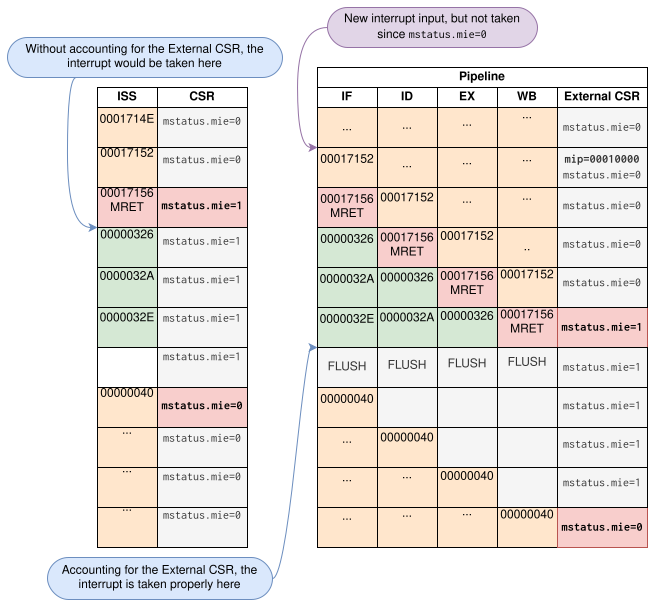
\includegraphics[width=1\linewidth]{figures/mret_example.pdf}
    \caption{Example showing how the timing of CSRs can influence interrupt timing.}
    \label{fig:mret_example}
\end{figure}

We see that in the ISS, the interrupt is not immediately taken after the \rv{mret} instruction since it also considers the external CSR, where \rv{mstatus.mie} is 0. When \rv{mret} reaches WB in the pipeline shell, the external CSR is updated, and the interrupt is taken. 

At this point, we have another problem with CSR timing. CSRs are not always updated in the WB stage. The example shows that in the external CSR, \rv{mstatus.mie} is high until the interrupt handler reaches WB. However, as seen in \Cref{fig:interrupt_timing}, the core immediately disables \rv{mstatus.mie} when an interrupt is taken.

Therefore, we define the \sv{interrupt_enabled} signal that is sent to the ISS with \sv{iss_intr()}. It should go high when \rv{mstatus.mie} reaches WB, and go low immediately after an interrupt is taken. This behavior is shown \Cref{fig:mstatus_mie}, which shows how the signal can be modeled using the \sv{wb_mstatus.mie} signal generated from the WB stage, and the \sv{interrupt_taken} returned from \sv{iss_intr()}.

\begin{figure}
    \centering
    \begin{tikztimingtable}
      \sv{clk}                  & 10{2C} G \\ 
      \sv{wb_mstatus.mie}       & LL   2{2H} 7{2L} \\ 
      \sv{interrupt_taken}      & 5{2L}  2{2H} 3{2L} \\ 
      \sv{interrupt_enabled}    & LL 6{2H} 3{2L} \\
    \end{tikztimingtable}
    \caption{Timing of \sv{interrupt_enable} and \sv{mstatus.mie}}
    \label{fig:mstatus_mie}
\end{figure}

The desired \rv{mstatus.mie} signal is shown in the combined CSR column in \Cref{fig:mret_example}, showing that \rv{mstatus.mie} is enabled when \rv{mret} reaches WB and disabled when the interrupt is taken the next cycle.

The previous example focuses on \rv{mstatus}, but the same problem can, for example, also occur immediately following a write to the \rv{mie} CSR that enables a previously disabled \rv{irq}. It can also be solved by storing \rv{mie} in the external CSR.

\section{Pipeline Flushing and ISS Revertion}

\subsection{Flushing}

As described in \Cref{sec:bg_flushing}, we must discard instructions already in the pipeline when the PC is changed by a jump, branch, or interrupt.
To model our pipeline shell, we will also need to implement pipeline flushing.

\subsubsection{Flush After Jump/Branch}

A typical pipeline flushes when the core jumps or branches to a new PC \cite{pattersonComputerOrganizationDesign2021}. Since we call the ISS in the IF stage, and the ISS fully executes one instruction before the next, the ISS always executes the correct instruction after a branch or jump, and we do not get the same incorrect instructions as the core in the pipeline that need to be flushed.

The CV32E40S core executes jumps in the ID stage and branches in the EX stage \cite{openhwgroupPipelineDetailsCOREV2023}. This means the core and reference model can mismatch the IF and ID stages before a jump or branch is correctly taken in the core. However, looking at \Cref{fig:dependency-tree-cv32x}, we see that the state of the IF is not required for interrupt timing and that the ID stage is only relevant for \acrshort{clic} interrupts. Since we, for the time being, only support \acrshort{clint} interrupts, we choose to ignore flushing the pipeline because of jumps and branches, but this assumption should be re-evaluated when implementing \acrshort{clic} interrupts in future work.


\subsubsection{Flushing After an Interrupt}

Since interrupts are asynchronous to the processor execution, we can not ignore the flushing caused by interrupts. When the interrupt is taken, the remaining instructions in the pipeline must be flushed. In our implementation, we clear the \sv{rvfi} data in each pipeline stage and set the \sv{valid} signal to 0. We use the \sv{if_flush, id_flush, ex_flush}, and \sv{wb_flush} from the controller to the pipeline stages to control flushing in each stage. When the ISS decides to take an interrupt, the \sv{iss_intr()} function returns true, and the \sv{interrupt_taken} signal is set. This signal can be output to the pipeline stages with the \sv{flush} signals.


%\begin{systemverilog}
%    assign flush_pipeline = interrupt_taken || debug_taken_q;
%
%    always_comb begin
%        if_flush_o <= flush_pipeline;
%        id_flush_o <= flush_pipeline;
%        ex_flush_o <= flush_pipeline;
%        wb_flush_o <= flush_pipeline;
%    end
%\end{systemverilog}


\section{State Revertion}
\label{sec:ps_revertion}

In a traditional pipeline, where the state changes are applied in the WB stage, flushing each pipeline stage is sufficient to discard the effects of the instruction \cite{pattersonComputerOrganizationDesign2021}.

However, in our reference model, the ISS executes an entire instruction before passing the result to the IF stage.
This means that the instruction's state changes are already applied within the ISS, and flushing the pipeline alone will not undo these changes. This is one of the significant disadvantages of calling the ISS in the IF stage compared to calling the ISS in the WB stage.

To address this and properly flush the pipeline shell, we need a mechanism to revert the state of the ISS to a previous state.
This involves restoring register values, \acrshort{csr}s, memory writes, and other relevant state information.

This is in some ways comparable to the rollback approach used by some lock-step processors \cite{marquesLockVHeterogeneousFault2021, liDuckCoreFaultTolerantProcessor2021, nikiemaDesignLowComplexity2023} to \textit{rollback} the processor context of two synced cores if they diverge. \textcite{marquesLockVHeterogeneousFault2021} saves a \textit{snapshot} of the state of the processor at various \textit{checkpoints} along the execution, and if a fault is found, the state is reverted to the previous valid checkpoint.

We can use a similar approach to store the state of the ISS into \textit{snapthots} we can revert back to. Since an interrupt and flush can happen at any instruction, we need a checkpoint between every instruction.


To properly revert the state of the ISS, we must be able to revert all possible external and state changes caused by executing an instruction. The most important registers are the 32 \acrfull{gpr} and the \acrfull{pc}, which are written to or read from at almost every instruction \cite{watermanRISCVInstructionSet2019}.
Some \acrfull{csr} are also changed because of instructions and must be stored. Many CSRs are likely to remain static like the \rv{mvendorid}, \rv{misa}, and \rv{marchid}, while others may change during execution like \rv{mstatus}, \rv{mie}, and \rv{mscratch} \cite{watermanRISCVInstructionSet2021}. Therefore, we must decide to only store some relevant CSRs or all CSRs.

Additionally, since we use the ISS's internal memory simulation, we need to revert potential memory writes that occurred for instructions that must be discarded.


\subsection{Store States in Pipeline Shell or ISS}

We can either store these states inside the ISS or in the Pipeline shell. By outputting the snapshot and moving it through the pipeline, it would theoretically be simple to input the state of the oldest instruction in the pipeline into the ISS and revert back to it. This could be more practical if a core-independent pipeline shell is chosen in \Cref{sec:ps_dependency}. In practice, converting the snapshot into SystemVerilog may be difficult, and it must be contained enough to be sent through the pipeline easily. %Another solution could be not to store the entire state as a snapshot but only store the state changes. This would require iterating through the pipeline stages in reverse and reversing all the stored state changes.

Instead, we choose to store the snapshot inside the ISS. This keeps the state contained and allows the snapshot to be stored in a logical format to the ISS without converting it to and from SystemVerilog to be sent through the pipeline. 
To revert the state from outside the ISS, we introduce a \sv{revert_steps} parameter to the \sv{iss_intr()} function. This parameter indicates the number of states to revert, allowing the ISS to revert the instructions flushed in a typical pipeline.
This gives us \Cref{issReq:revertState}, specifying that the ISS must be able to revert to a previous state, reverting registers, CSRs, and memory operations.

\subsection{When To Revert}
\label{sec:ps_when_revert}

The order of events when reverting the state is essential to get right.
The naive order could look something like this:

\begin{enumerate}
    \item An interrupt is input into the reference model
    \item The reference model decides if the interrupt is allowed and inputs the \rv{irq} bits into the ISS with \sv{iss_intr()}
    \item The ISS reports that the interrupt is taken
    \item The pipeline shell is flushed
    \item We revert the ISS to a previous state
    \item The ISS starts running the interrupt handler
\end{enumerate}

This order is problematic. When we run the \sv{iss_intr()} function and the interrupt is taken in the ISS, this sets the \rv{mepc} and \rv{mstatus} CSRs as explained in \Cref{sec:bg_interrupts}. Reverting the state after the interrupt is taken in the ISS, like above, discards these CSR writes since the CSRs are reverted to a previous state. Since interrupt taking is decided inside the ISS, we can also not revert the state before running the \sv{iss_intr()} function.

To overcome this, we must revert the state before setting the \rv{mip}, but after deciding that the interrupt will be taken. We choose to revert the state from inside the ISS, instead of using a separate \sv{iss_revert()} function from the pipeline shell. Therefore, we add a \sv{revert_steps} parameter to the \sv{iss_intr()} function so that state revertion can be done inside the ISS.

This gives us the following order:

\begin{enumerate}
    \item An interrupt is input into the reference model
    \item The reference model decides if the interrupt is allowed and inputs the \rv{irq} bits into the ISS with \sv{iss_intr()}
    \item The ISS decides the interrupt will be taken
    \item The ISS reverts the state
    \item  The ISS takes the interrupt and writes to the relevant CSRs
    \item The pipeline shell is flushed
    \item The ISS starts running the interrupt handler
\end{enumerate}

\subsection{How Many States To Revert}

\begin{figure}
    \centering
    \includegraphics[width=0.85\linewidth]{figures/revert_example.pdf}
    \caption{Example showing how many instructions we need to revert the state when flushing the pipeline after.}
    \label{fig:revert_example}
\end{figure}


We can use the example in \Cref{fig:revert_example} to determine the number of steps to revert.
This shows the PC of the instructions in the pipeline shell and the PC of instructions executed in the ISS. In the WB stage, we see the retired instructions in bold, which are output over RVFI. An interrupt is applied when \sv{1504} retires, and the reference model decides that interrupts are allowed and calls the ISS with \sv{iss_intr()}. Since \sv{1504} is the last instruction to retire, we need to discard the changes from \sv{150a}, \sv{1508}, and \sv{1506} by reverting the state of the ISS to the state before it executed \sv{1506}. After the reversion is done, the ISS can take the interrupt, and \sv{1506} will be stored in the \rv{mepc} CSR and be the first instruction to run when the interrupt handler is completed.

With our current retirement-dependent implementation, we must always revert the same number of instructions for a given number of pipeline stages since we always step the ISS in conjunction with the pipeline. However, we would likely need to revert a variable number of instructions for a core-independent approach. For our implementation of the CV32E40S core with four pipeline stages, we see from the figure that we always need to revert three instructions.



%
%\begin{figure}[htb]
%\centering
%\input{figures/interrupt_revert_tikz}
%\caption{\tmp{TODO: fix figure}Illustrate state reversion with ISS content and pipeline content.}
%\label{fig:interrupt_revert_addi}
%\end{figure}
%
%\begin{figure}[htb]
%\centering
%\begin{ganttchart}[
		x unit=1.4cm,
		y unit chart=0.7cm,
		canvas/.style={draw=none,fill=none}, % remove canvas borders, etc
		vgrid={*{2}{draw=black!8}},           % vertical gray lines every unit
		inline,                              % draw bars inline
		group/.style={draw=none,fill=none},  % remove group borders, etc
		bar top shift=0.1,                   % give bar 10% padding top/bottom
		bar height=0.8,                      % bar size 80% of vertical space
		y unit title=0.5cm,                  % crop titles a little smaller
		title/.style={draw=none,fill=none},  % remove title borders, etc
		include title in canvas=false        % no vertical grid in title
	]{-2}{4}

    %\gantttitlelist{Cycle,IF,ID,EX,WB}{1}

	\gantttitle{Cycle}{-1}
	\gantttitle{ISS}{3}
 
	\gantttitle{}{1}
	\gantttitle{IF}{-1}
	\gantttitle{ID}{3}
	\gantttitle{EX}{-1}
	\gantttitle{WB}{3} \\

	\ganttgroup[inline=false]{1}{0}{4}
	\ganttbar[bar/.style={draw=black!80,fill=orange!40},name=iss0 ]{1}{-2}{-2}
	\ganttbar[bar/.style={draw=black!80,fill=orange!40}  ]{1}{0}{0}\\
 
	\ganttgroup[inline=false]{2}{0}{4}
	\ganttbar[bar/.style={draw=black!80,fill=yellow!40}, name=iss1  ]{2}{-2}{-2}
	\ganttbar[bar/.style={draw=black!80,fill=yellow!40}  ]{2}{0}{0}
	\ganttbar[bar/.style={draw=black!80,fill=orange!40}  ]{1}{1}{1}\\
 
	\ganttgroup[inline=false]{3}{0}{4}
	\ganttbar[bar/.style={draw=black!80,fill=lime!40},name=iss2    ]{3}{-2}{-2}
	\ganttbar[bar/.style={draw=black!80,fill=lime!40}    ]{3}{0}{0}
	\ganttbar[bar/.style={draw=black!80,fill=yellow!40}  ]{2}{1}{1}
	\ganttbar[bar/.style={draw=black!80,fill=orange!40}  ]{1}{2}{2}\\
 
	\ganttgroup[inline=false]{4}{0}{4}
	\ganttbar[bar/.style={draw=black!80,fill=green!40},name=iss3   ]{4}{-2}{-2}
	\ganttbar[bar/.style={draw=black!80,fill=green!40}   ]{4}{0}{0}
	\ganttbar[bar/.style={draw=black!80,fill=lime!40}    ]{3}{1}{1} 
	\ganttbar[bar/.style={draw=black!80,fill=yellow!40}  ]{2}{2}{2} 
	\ganttbar[bar/.style={draw=black!80,fill=orange!40}  ]{1}{3}{3} 
	\ganttbar[bar/.style={draw=none}  ]{\textbf{valid}}{4}{4} \\
 
	\ganttgroup[inline=false]{5}{0}{4}
    \ganttbar[bar/.style={draw=black!80,fill=cyan!40},name=iss4    ]{5}{-2}{-2} 
    \ganttbar[bar/.style={draw=black!80,fill=cyan!40}    ]{5}{0}{0} 
	\ganttbar[bar/.style={draw=black!80,fill=green!40}   ]{4}{1}{1}
	\ganttbar[bar/.style={draw=black!80,fill=lime!40}    ]{3}{2}{2} 
	\ganttbar[bar/.style={draw=black!80,fill=yellow!40}  ]{2}{3}{3}  
	\ganttbar[bar/.style={draw=none}  ]{\textbf{valid}}{4}{4} \\

	\ganttgroup[inline=false]{6}{0}{4}
    \ganttbar[bar/.style={draw=black!80,fill=cyan!40}    ]{5}{0}{0} 
	\ganttbar[bar/.style={draw=black!80,fill=green!40}   ]{4}{1}{1}
	\ganttbar[bar/.style={draw=black!80,fill=lime!40}    ]{3}{2}{2} 
	\ganttbar[bar/.style={draw=black!80,fill=yellow!40}  ]{2}{3}{3}  
	   \\

	\ganttgroup[inline=false]{(IRQ) 7}{0}{4}
    \ganttbar[bar/.style={draw=black!80,fill=cyan!40}    ]{5}{0}{0} 
	\ganttbar[bar/.style={draw=black!80,fill=green!40}   ]{4}{1}{1}
	\ganttbar[bar/.style={draw=black!80,fill=lime!40}    ]{3}{2}{2} 
	\ganttbar[bar/.style={draw=black!80,fill=yellow!40}  ]{2}{3}{3}  
	\\



	\ganttgroup[inline=false]{(Revert(3)) 8}{0}{1}
    \ganttbar[bar/.style={draw=black!80,fill=black!10},name=issRev    ]{3}{-2}{-2} 
    \ganttbar[bar/.style={draw=black!80,fill=black!10}    ]{}{0}{0} 
    \ganttbar[bar/.style={draw=black!80,fill=black!10}    ]{}{1}{1} 
    \ganttbar[bar/.style={draw=black!80,fill=black!10}    ]{}{2}{2} 
    \ganttbar[bar/.style={draw=black!80,fill=black!10}    ]{}{3}{3} 
    
    \\
    
	\ganttgroup[inline=false]{9}{0}{1}
	\ganttbar[bar/.style={draw=black!80,fill=red!50}]{IH1}{-2}{-2}
	\ganttbar[bar/.style={draw=black!80,fill=red!50}]{IH1}{0}{0} \\

	\ganttgroup[inline=false]{10}{0}{1}
	\ganttbar[bar/.style={draw=black!80,fill=orange!80}    ]{IH2}{-2}{-2}
	\ganttbar[bar/.style={draw=black!80,fill=orange!80}    ]{IH2}{0}{0}
	\ganttbar[bar/.style={draw=black!80,fill=red!50}       ]{IH1}{1}{1} \\
	
	\ganttgroup[inline=false]{11}{0}{1}
	\ganttbar[bar/.style={draw=black!80,fill=yellow!80}    ]{IH3}{-2}{-2}
	\ganttbar[bar/.style={draw=black!80,fill=yellow!80}    ]{IH3}{0}{0}
	\ganttbar[bar/.style={draw=black!80,fill=orange!80}    ]{IH2}{1}{1}
	\ganttbar[bar/.style={draw=black!80,fill=red!50}       ]{IH1}{2}{2} \\
 
	\ganttgroup[inline=false]{12}{0}{1}
	\ganttbar[bar/.style={draw=black!80,fill=lime}       ]{IH4}{-2}{-2}
	\ganttbar[bar/.style={draw=black!80,fill=lime}       ]{IH4}{0}{0}
	\ganttbar[bar/.style={draw=black!80,fill=yellow!80}    ]{IH3}{1}{1}
	\ganttbar[bar/.style={draw=black!80,fill=orange!80}    ]{IH2}{2}{2}
	\ganttbar[bar/.style={draw=black!80,fill=red!50}       ]{IH1}{3}{3}  
	\ganttbar[bar/.style={draw=none}  ]{\textbf{valid}}{4}{4}\\


    \ganttlink[]{iss2}{issRev}

    %\ganttlink[link type=rdldr]{[xshift=-0.3cm]iss3.east}{[yshift=1cm]iss3.east}{[yshift=1cm]iss2.east}
    %\ganttlink[]{[yshift=1cm]iss4.east}{[yshift=1cm]iss3.east}

\end{ganttchart}

%\caption{\tmp{TODO: fix figure} Illustrate state reversion with ISS content and pipeline content.}
%\label{fig:interrupt_revert_divu}
%\end{figure}




\section{Other Asynchronous Events}% : \Cref{psReq:async_control}}
\label{sec:other_async}

Since the previous sections used interrupts as an example of how asynchronous events can be handled in the pipeline shell, this section will cover how the techniques and design choices discussed for interrupts can also be applied to other asynchronous events.


\subsection{Applying Interrupt Handling Techniques To Debug Requests}

%We will use debug requests as an example of how other asynchronous events can utilize the techniques discovered for interrupts.
%
%As explained in \Cref{sec:bg_debug}, debug requests allow developers to gain visibility and control over the processor's execution.

The CV32E40S core \cite{openhwgroupDebugTriggerCOREV2023} supports the RISC-V Debug Specification from \cite{pauldonahueRISCVDebugSupport2023}, which defines a standard interface for debugging. In CV32E40S, debug requests can be triggered synchronously through \rv{ebreak} instructions or asynchronously through the \sv{debug_req_i} input. \sv{debug_req_i} can be thought of as the "debug interrupt" \cite{openhwgroupDebugTriggerCOREV2023}, interrupting normal program execution and changing to a debug handler. When the debug is \textit{taken}, the core enters debug mode and saves the current \acrshort{pc} and other relevant state information.

Debug requests share many similarities with interrupt handling. Both are asynchronous events interrupting the processor's operation, and both require the pipeline to be flushed and the processor's state to be saved before the event can be handled. The following sections will cover how the techniques for interrupts apply to debug requests.  

\subsubsection{Informing the ISS of Debug Requests}

We can inform the ISS of debug requests the same way as interrupts in \Cref{sec:ps_interrupt} by using a \sv{iss_set_debug(...)} function called every cycle. This can work similarly to \sv{iss_intr(...)}, taking \sv{debug_req_i} and \sv{debug_allowed} as inputs.

The \sv{debug_allowed} signal is used like the \sv{interrupt_allowed} signal and is determined by the pipeline shell based on the current processor state. If debug is allowed, the ISS decides whether to take it, storing the necessary state information and entering debug mode.


\subsubsection{State Reversion After Debug}

Similar to interrupts, when an external debug request is taken, the pipeline must be flushed, and the PC needs to be changed to the debug handler. 

This gives the same problem as interrupts in \Cref{sec:ps_revertion}, where the ISS needs to be reverted to a previous state. This can be implemented the same way as for interrupts, where the \sv{iss_set_debug()} function takes in the number of states to revert and reverts the state if the debug request is taken. 

\subsubsection{Delay Debug Mode With Pipeline}

The debug mode of the processor causes a similar problem to the timing of \rv{mstatus.mie} explained in \Cref{sec:ps_side-effects}, where the value changes too early in the ISS and needs to be delayed with an external CSR. Similar to the \rv{mret} example in \Cref{fig:mret_example_fail}, the same problem can occur when a debug handler returns with the \rv{dret} instruction and immediately goes straight into another debug request. 
This can be solved the same way as for interrupts by outputting the \rv{debug_mode} from the ISS over RVFI, propagating it through the pipeline, and storing it similarly to the external CSR. 
This value is passed to the ISS with the \sv{iss_set_debug()} function and considered by the ISS before taking a debug request.


%\subsubsection{Two debug requests after each other}
%
%We get the same problem when a debug request returns from debug mode with \rv{dret} and goes straight into another debug request, as when an interrupt returns from the interrupt handler with \rv{mret} and takes another interrupt. The problem here is that the ISS runs a few instructions ahead and applies the side effects of the \rv{dret} instruction prematurely, causing the \sv{iss_set_debug()} function to set \sv{debug_taken} and flush the pipeline prematurely.
%
%This is solved for interrupts by exporting the relevant CSRs through RVFI, passing them through the pipeline to an external CSR, and using these to correctly time the changes.
%
%\rv{dret} restores the PC and privileged to the values stored in \rv{dpc} and \rv{dcsr}, and exits debug mode. The side effect that influences the timing of debug requests is that \ccode{debug_mode} is turned off in \rv{dret}. the \ccode{debug_mode} is used by the \ccode{set_debug} method to determine if a new debug request can be made, or if the processor is currently in the debug mode. We must therefore delay this signal to when the pipeline shell is out of debug mode, and not only when spike has exited debug mode. 
%
%The debug mode is output to RVFI via the \sv{rvfi_dbg_mode} signal. One solution is therefore to use this to update a copy of \sv{debug_mode} in the pipeline shell. One problem with this is that the \sv{rvfi_dbg_mode} reports high when in \rv{dret} since the instruction is run in debug mode, but since \rv{dret} disables debug mode, we want to set our local copy to 0 when the \rv{dret} instruction leaves WB. 
%
%\tmp{TODO: solve this. Pass a separate dbg mode signal through the stages, update internally in spike with saved states, or have a special "if dret" signal to set debug mode to 0}
%
%\subsection{debug at the very start}
%
%\tmp{Debug asserted from the beginning causes problems with state revertion, since it tries to revert more instructions than are stored in the previous states.}

\subsection{Interrupts and Debug Requests Simultaneously }

When interrupts and debug requests occur simultaneously, this can also lead to more problems. One example is when we return from debug mode and immediately take an interrupt.
The same way the changes from \rv{mret} must be delayed in an external CSR in \Cref{fig:mret_example}, the state changes from \rv{dret} must also be considered before taking an interrupt. This requires that the current debug mode is also considered before taking an interrupt.
When considering multiple asynchronous events, we can not separate the handling of interrupts and debug requests since these affect each other.

\subsection{Non Maskable Interrupts (NMIs)}

To limit the scope of this thesis, \acrfull{nmi} are not implemented. However, we will briefly discuss how NMIs could work in our design.

\acrfull{nmi} operate similarly to normal interrupts, by updating \rv{mepc}, \rv{mcause}, and \rv{mstatus} CSRs. 
In the CV32E40S core, NMIs are also controlled with similar \sv{pending_nmi} and \sv{nmi_allowed} signals as interrupts \cite{openhwgroupCv32e40s2024}. However, NMIs are not masked by the \rv{mie} CSR bits but will be masked in debug mode. Additionally, NMIs caused by an instruction allow this instruction to be retired before taking the NMI \cite{openhwgroupExceptionsInterruptsCOREV2023}. 

We imagine that the following techniques can be transferrable to NMIs:

\begin{itemize}
    \item \textbf{Informing the ISS of NMIs:} We can use a \sv{iss_set_nmi()} function similarly to interrupts, taking \sv{pending_nmi} and \sv{nmi_allowed} signals.
    \item \textbf{State reversion after NMI:} Similar to interrupts, NMIs also require the pipeline to be flushed when taken. The same state revertion technique as interrupts can likely be used to revert the state when an NMI is taken.
    \item \textbf{Delaying CSRs through the pipeline:} Since NMIs are not masked by \rv{mie}, and \rv{mstatus} we do not need to delay these CSRs with an external CSR. NMIs are, however, masked by the debug mode, so \sv{iss_set_nmi()} may need to take \sv{debug_mode} as an input. 
\end{itemize}


\subsection{Prioritizing Events}

We also have to prioritize the different asynchronous events in relation to each other. Since we currently use the ISS to determine which asynchronous event to take, it must also consider the prioritization between the different events. The prioritized list of the CV32E40S \cite{openhwgroupCv32e40s2024} is shown below and may need to be configured in the ISS to choose the correct asynchronous event.

\begin{enumerate}
    \item NMIs
    \item Asynchronous debug requests (\sv{debug_req_i})
    \item Interrupts
    \item Synchronous debug requests (\rv{ebreak})
    \item normal execution
\end{enumerate}



%\subsection{CLIC Interrupts}
%
%CLIC and CLINT both use the same \sv{pending_interrupt} and \sv{interrupt_allowed} signals but differ in how they take the interrupt.
%
%\subsection{NMI}
%
%\sv{pending_nmi} and \sv{nmi_allowed}.
%\sv{nmi_allowed} is equal to \sv{interrupt_allowed}, except \sv{!interrupt_blanking_q} is replaced by \sv{!(woke_to_debug_q || woke_to_interrupt_q)}
%
%
%
%
%
%
%\subsection{Similarities to CLINT interrupts}
%
%From above we see that \sv{lsu_interruptible_i}, \sv{fencei_ongoing clic_ptr_in_pipeline}, \sv{sequence_interruptible}, \sv{csr_flush_ack_q}, and \sv{ctrl_fsm_cs} are all common signals for \sv{interrupt_allowed}, \sv{async_debug_allowed}, and \sv{nmi_allowed}. The pipeline contents influence these signals, and solving how these can be used to properly time the asynchronous events is common for all of these events.
%
%
%By using CLINT interrupts as an example to verify if this approach for determining if an interrupt can be taken works, we can also assume that the same result will apply to CLIC interrupts, debug requests, and \acrshort{nmi}s by using \sv{async_debug_allowed}, \sv{nmi_allowed}, etc. 
%


%\subsection{WFI}
%
%\tmp{TODO}
%
%\tmp{We disable wifi in the ISS so that the timing is done in the pipeline shell}


\subsection{WFI}
\label{sec:wfi}

A \rv{wfi} instruction should halt execution until an interrupt occurs \cite{watermanRISCVInstructionSet2021}. This requires some modifications to the design to function correctly.

One problem with \rv{wfi} instructions and the pipeline shell is that the next steps in Spike will not be executed when a \rv{wfi} is set. This prohibits the pipeline from filling up with the upcoming instructions. When an interrupt is taken, and \rv{wfi} is awakened, the next instructions are not loaded into the pipeline, causing a mismatch. To avoid this, we fully disable \rv{wfi} in the ISS and let the pipeline shell handle the waiting caused by a \rv{wfi}. This is legal since the RISC-V specification also specifies that implementing \rv{wfi} as a \rv{nop} is a legal implementation \cite{watermanRISCVInstructionSet2021}. As will be discussed in \Cref{sec:res_tests}, this causes some problems when a \rv{wfi} is the last instruction of a program.


%\subsection{EBREAK in pipeline when external debug request is enabled}
%\tmp{I PS?}
%
%Since the ISS is run in IF, when an \rv{ebreak} instructions runs in IF, the ISS sets debug mode to 1. This causes problems for a debug request asserted while the \rv{ebreak} is in the pipeline, but not yet executed in WB. Since the ISS already is in debug mode caused by the \rv{ebreak}, the debug request would not be taken, and the cause of the debug mode would be the \rv{ebreak} instead of the external debug request, which has a higher priority. To fix this, we can modify \ccode{set_debug()} to check if a new debug request is made while the debug mode is not set in the pipelines shell but is set in the ISS, and the current debug cause is by an \rv{ebreak}. This only occurs if the \rv{ebreak} is still in the pipeline. If this is the case, we can disable debug mode, so that the external debug request can trigger debug mode again with the correct cause.




\chapter{Instruction Set Simulator (ISS)}
\label{ch:ISS}

%\tmp{Burde jeg delt opp kapittelet tydeligere i: 1. Adding CV32E40S support to spike, og 2. Modifications to support pipeline shell??}

The \acrfull{iss} is a critical component in our reference model, responsible for the functional execution of each instruction While the pipeline shell handles the timing and core-specific pipeline behaviour, the ISS ensures the correct interpretation and execution of the instructions according to the RISC-V ISA specification \cite{watermanRISCVInstructionSet2019, watermanRISCVInstructionSet2021}.

This chapter will discuss the selection and modification of the iSS to meet the requirements of our reference model. cover the necessary modifications to the ISS to integrate it with the rest of the design. The key contributions in this chapter can be categorized into two main areas:

\begin{enumerate}
    \item Modifying the ISS to support the CV32E40S processor core.
    \item Modifying the ISS to ensure proper interaction with pipeline shell.
\end{enumerate}

\section{ISS Requirements}

To achieve these goals, we define the following requirements for the ISS. These requirements are collected from the previous chapters and referred to as \textbf{ISS Requirement X}.


and are required for the ISS to be used as a part of the reference model. This chapter will use these requirements to discuss the choice of ISS and its necessary modifications. 

\begin{enumerate}

%\item \textbf{Provide visibility into multiple instructions} \label{issReq:visibility}
%
%\par To simulate the pipeline, we need to track multiple instructions simultaneously, corresponding to the instructions in the different pipeline stages. This requires that we can "see" the $n$ coming instructions according to the pipeline stages, or allow separation of fetching, decoding, execution, etc into separate cycles. 

\item \textbf{The ISS should be easily replaceable in the future.} \label[issReq]{issReq:replacable}

\par The ISS should be mature and thoroughly tested. It should be actively maintained and likely to be updated in the future.

\item \textbf{The ISS should be core-independent} \label[issReq]{issReq:coreIndependent}

\item[] The ISS should contain as little core-dependent functionality as possible to make the reference model easily modifiable to different cores.

\item \textbf{Modify ISS to match the core.} \label[issReq]{issReq:csr}

\item[]  The ISS should be able to be modified to match the core. Specifically regarding memory mapping and CSRs.

\item \textbf{Run \acrshort{riscv} binaries generated from core-v-verif.} \label[issReq]{issReq:binaries}

\item[]  The ISS must be able to run the same binaries as the core.

\item \textbf{Support stepping through the execution at the Instruction Level} \label[issReq]{issReq:step}

\item[]  Since the reference model runs in lock-step with the DUT, we need to be able to step through the instructions at the instruction level, and be able to only run one instruction at a time, before waiting to step into the next instruction.

\item \textbf{Provide processor state after each instruction} \label[issReq]{issReq:state}

\par The ISS needs to output the state changes executed after each instruction so that the pipeline shell can apply these changes in a cycle-accurate manner. 
%To be able to use the ISS in verification, we need to access the processor state changes after each instruction to compare with the DUT. This should preferably be in the RVFI format or enough information should be available to convert into an RVFI item.

\item \textbf{Revert the state of the ISS a variable number of instructions} \label[issReq]{issReq:revertState}

\par To discard instructions flushed in the pipeline, we must be able to revert the ISS to a previous state, as discussed in \Cref{sec:ps_revertion}. We must be able to revert the \acrshort{pc}, \acrshort{gpr}, \acrshort{csr}, and memory operations a set number of steps.


%\item \textbf{Support modification of instructions} \label[issReq]{issReq:modification}
%
%\par To simulate interrupts in the pipeline, it might be necessary to simulate pipeline flushing and halting. To do this we should be able to modify the instructions in the pipeline e.g. to replace them with empty NOP operations to flush the pipeline or halt execution of an instruction. 

\item \textbf{Enable external injection of interrupts} \label[issReq]{issReq:interrupt} 

\par External interrupts and debug requests are inserted into the reference model independently of the ISS. To simulate the interrupts, we must be able to tell the ISS to take an interrupt by jumping to the trap handler's PC and correctly executing the side effects at the correct cycle. 

\item \textbf{The ISS should decide which interrupt to take, when multiple interrupts are enabled} \label[issReq]{issReq:interruptOrdering} 

\par As discussed in \Cref{sec:ps_interrupt}, which interrupt to take should be decided in the ISS instead of the pipeline shell. This means that the ISS must also know the interrupt ordering of the custom interrupts in bit 16 and above, in addition to the ordering of bit 15:0 specified in the RISC-V specification.

\item \textbf{Enable and disable interrupt independently of the \rv{mip} bits} \label[issReq]{issReq:interruptEnabled} 

\par The \rv{mip} bits should be able to be set without necessarily triggering an interrupt.

\item \textbf{Configurable with different extextions} \label[issReq]{issReq:custom}

\par A large driving force for using RISC-V is the ability to add custom extensions. Therefore, custom instructions and extensions must be easily created and added to the ISS without modifying large parts of the model.

%\item \textbf{Ensure maintainability while meeting requirements} \label[issReq]{issReq:update}
%
%\par The ISS should be easily maintained and updated while still meeting the requirements. Modifications to the ISS should be kept to a minimum and be done in a way that allows the ISS to be easily updated.

%\item \textbf{Actively maintained and thoroughly tested} \label[issReq]{issReq:maintained}

%\par The ISS should be mature and thoroughly tested. It should be actively maintained and likely to be updated in the future.


\item \textbf{Output CSRs relevant for interrupt timing.} \label[issReq]{issReq:CSR_out}

\par The ISS should output the CSRs that have an influence on interrupt timing, so that these can be applied at the correct time. This includes the \rv{mstatus.mie} and \rv{mie} CSRs.

\item \textbf{Set interrupt dependent CSRs from outside of the ISS.} \label[issReq]{issReq:set_CSR}

\par We should be able to apply the effects of the \rv{mie} and \rv{mstatus} CSRs from outside of the ISS, to ensure interrupts are timed correctly.

\item \textbf{[optional] The ISS should compatible with formal verification} \label[issReq]{issReq:formal}

\par The ISS should be compatible with formal verification by being able to compile into synthesizable RTL code.
%\item \textbf{Load the same instructions as the DUT} \label[issReq]{issReq:DUTins}

%\par The ISS should be able to load the same instructions as the DUT.

%\par As discussed in \cref{sec:shell_iss_interaction}, to be able to model the reference model around an ISS, it is helpful to be able to separate the register file from the rest of the ISS, or be able to have a copy of the register file, and update the register file inside the ISS when necessary.

\end{enumerate}

\section{Choosing ISS}

The specialization project discussed multiple potential \acrshort{iss}s in \Cref{sec:pw_iss} and found that Spike \cite{SpikeRISCVISA2023} and sail-riscv \cite{RISCVSailModel2023} were the most viable choices. Both of these pass many of the requirements above, but Spike was thought to be the easiest to get started with and integrate with the rest of the pipeline shell. 

The deciding factor for us is whether any of the ISSs can meet \Cref{issReq:formal} and be synthesizable. Spike is written in \cpp and is not synthesizable. 

Sail-riscv is written in the Sail language. Sail recently added support for compiling the model to SystemVerilog code\footnote{\url{https://github.com/rems-project/sail/releases/tag/0.17}}. If the model could generate synthesizable SystemVerilog code, this would meet \Cref{issReq:formal}. This feature is however still very experimental, and at the time of writing not yet implemented into the sail-riscv model\footnote{\url{https://github.com/rems-project/sail/issues/420}}.
When this feature is implemented in the future, this would be very interesting future work to implement, but for now, we choose to go with Spike.
We will adhere to \Cref{issReq:replacable} and make the ISS replaceable, in order to make this potential switch easy in the future


There are multiple Spike forks that we can choose to use. One potential version of Spike to use is a version that is already part of core-v-verif and is used to verify the CVA6 core from the OpenHW group. This Spike implementation is still in active development but adds some advantageous features for integrating it into the reference model.

To meet \Cref{issReq:step}, the ISS has to be able to step through the instructions, one instruction at a time. It must also output the processor state as RVFI to comply with \Cref{issReq:state}. The normal version of Spike runs sequentially, so some requirements are necessary to do this. These are the most important modifications done to the Spike version for CVA6. It implements a set of DPI function calls that are used to step through instructions in Spike and returns a simplified RVFI output \cite{openhwgroupOpenhwgroupCorevverif2023}.

These are implemented in the \file{riscv_dpi.cc} file that has DPI functions for setting parameters, initializing Spike, and stepping through the model. To maintain the state, this file has several classes instantiated as global variables, the most important being \ccode{Simulation* sim}, which is an addition made with the CVA6 Spike implementation. The \ccode{Simulation} class inherits from the spike \ccode{sim_t} class and adds a lot of the functionality implemented in the main function in pure Spike.  



\begin{table}[!htb]
\centering
%\setlist[itemize]{font= \color{DeepSkyBlue}, wide, leftmargin=*, noitemsep, after=\vspace*{-\topsep}}
%\setlength{\extrarowheight}{3pt}
%\setlength{\tabcolsep}{3pt}
\caption{Summary of advantages and disadvantages of Plain Spike and CVA6 Spike}
\label{tab:spikevsail}
%\begin{tabularx}{\textwidth}{|p{15mm}|*{2}{>{\compress\RaggedRight\arraybackslash} X |}}
\begin{tabularx}{\textwidth}{|p{15mm}|*{2}{>{\arraybackslash} X |}}
\hline
ISS & Advantages & Disadvantages \\
\hline
Plain Spike
& \begin{itemize}
\item Widely used and tested 
\item Stable 
\item Easier to keep up to date with changes to Spike
\end{itemize}
& \begin{itemize}
\item No support for RVFI outputs
\item Interrupt and debug injection must be added
\item DPI support must be added
\end{itemize} \\
\hline
CVA6 Spike
& \begin{itemize}
\item Supports a minimala version of RVFI 
\item Built into the core-v-verif
\item Already modified to work with DPI functions from systemverilog
\end{itemize}
& \begin{itemize}
\item Modified for the CVA6 Core
\item Currently in active development, so interfaces and functionality can change in the future
\item Not available in the same core-v-verif branch used by the CV32E40S/X cores which can get ugly.
\end{itemize} \\
\hline
\end{tabularx}
\end{table}







%\section{Memory regions}
%
%Spike needs to be configured to use the same memory regions as the test binaries.
%
%The binaries are generated using \lstinline{link.ld}
%
%This linkscript sets ram from \lstinline{0x00000000}
%
%by changing this to something else spike no longer complains, but the configuration of the processor changes.
%
%
%Spike configures a debug module from 0x0 to 0x1000 and a reset vector from 0x1000 to 0x2000 (REF mail. Sjekk opp). This overlaps with the memory description from link.ld and needs to be removed.
%
%
%One fix in link.ld:
%move ram to 0x80000000 and \lstinline{boot_address = 0x80000080}.
%set \lstinline{boot_addr_i = 0x80000080}.
%This kind of works, but we should modify spike instead of link.ld.




%\section{Experiment}
%
%\subsection{pure spike with cv32e40s test}
%memory 0x0 invalid
%
%\subsection{CVA6 test elf on pure spike}
%works
%
%\subsection{cva6 spike with cv32e40s test}
%memory 0x0 invalid
%
%
%\subsection{Move ram in link.ld to another location}
%Spike runs but core testbench fails




\subsection{Using CVA6 spike}

We choose to go with CVA6 spike implementation, but this also requires some modifications to be compatible with CV32E40S, and is one of the contributions of this thesis.

%Some modifications to CVA6 spike are necessary
%\begin{itemize}
%    \item Change memory mapping to handle cv32e40s binaries 
%    \item \lstinline{CV_VP_REGISTERs} are from \lstinline{0x00800000} and contain registers like virtual printer used by stdout and other thing.
%    \item  disable dtb to disable the spike bootloader that overlaps with core-v memory regions
%    \item Modify CSR registers
%\end{itemize}



\section{Making the ISS replaceable : ISS Requirement \ref{issReq:replacable} }

\subsubsection{ISS interface}

To easily interface with the ISS the communication is done in \file{iss_wrap_pkg.sv}. This exports the generic functions \lstinline{iss_init(...)} and \lstinline{iss_step(...)}) that "easily" allows the ISS the be replaced in the future by only modifying \lstinline{iss_wrap_pkg.sv}. The \lstinline{iss_init(...)} configures Spike with the correct ISA string, sets the boot address, sets the correct parameters and loads the ELF binary. 

\lstinline{iss_step(...}) steps spike one instruction and returns an \lstinline{st_rvfi} rvfi struct.

\tmp{More on the interface}

\section{Matching the ISS to the core: ISS Requirement \ref{issReq:csr} \& \ref{issReq:binaries}}

\subsection{Parameters}

The core-v-verif Spike version has implemented passing of parameters to Spike, and exports functions like \ccode{spike_set_param_str(base,string,value)}, and \ccode{spike_set_param_uint64_t(base,string,value)}\cite{openhwgroupOpenhwgroupCorevverif2023}. It also exports \ccode{spike_set_default_params(profile)}, that allows spike to be configured to different processors. 

We can call these function from \ccode{iss_init(...)} to configure the necessary modifications required to match the core. The necessary modifications will be discussed below. 

\subsection{Mismatched CSRs}

There are some differences in the implementation of the CSRs from the core and Spike. This happens because the RISC-V specification is not always fully accurate, and provides some optional implementations of some CSRs \cite{watermanRISCVInstructionSet2021} and some CSRs are specific to a core. Some necessary modifications are described below.

\begin{itemize}
    \item \rv{mvendorid}  - This is specific to the vendor and should be reset to the OpenHW vendor ID (\lstinline{0x602}) 
    \item \rv{marchid} - This is unique to each microarchitecture from a vendor. It should be reset to CV32E40S marchid (\lstinline{0x15})
    \item \rv{misa} - Spike does not have bit 23 set, which should be set if non-standard extensions are present\cite{watermanRISCVInstructionSet2021}. The CV32E40S hard-wires this to 1. We can add the "xdummy" to the ISA string passes to spike, so spike sets bit 23 high.
    \item \rv{mcountinhibit} - This should be reset to 5 instead of 0
    \item \rv{mcycle, mcycleh} - Disabeling of mcycle was not implemented in Spike. This required a modification to Spikes functionality to take mcountinhibit into account and only increase \rv{mcycle} if it is enabled.
\end{itemize}

%Mstatus differs this is from \cite{watermanRISCVInstructionSet2021}:
%M-mode software can determine whether a privilege mode is implemented by writing that mode
%to MPP then reading it back.
%If the machine provides only U and M modes, then only a single hardware storage bit is
%required to represent either 00 or 11 in MPP.


\subsection{Memory Mapping}

In order to run the same binaries as the core and fulfill \Cref{issReq:binaries}, Spike must be modified with the same memory mapping as the core.


%\url{https://github.com/openhwgroup/core-v-verif/tree/master/cv32e40s/bsp}
The binaries used in core-v-verif is built using the \acrfull{bsp} provided with core-v-verif in \dir{cv32e40s/bsp}. Among other things, this contains a linker script (\file{link.ld}) that defines the memory layout of the program, specifying the placement of code and data in memory \cite{openhwgroupCorevverifCv32e40sBsp}. 

The core-v-verif linker script has two sections, \lstinline{ram} and \lstinline{dbg}. The ram starts at address \lstinline{0x0} and has a size of \lstinline{0x400000} (4MB). The debug section starts at \lstinline{0x1A110800} and has a size of \lstinline{0x1000}. Additionally, the core has memory regions for virtual periphery registers and \lstinline{0x00800000}.

%To make Spike work with this new memory mapping we have to do the following:
%
%\begin{enumerate}
%    \item Remove spikes default memory mapping which overlaps with our new memory mapping.
%    \item Configure spike with the new memory mapping
%    \item Make spike start execution at the start address of \file{link.ld}.
%\end{enumerate}


Spike always starts running at the \lstinline{DEFAULT_RSTVEC = 0x1000}. Spike places a custom boot rom at this reset location \cite{evancoxAddDocumentationLowlevel2017}.
After this is run, spike will jump to the provided program counter or to the \lstinline{_start} symbol from the ELF file. Aditionally, spike has a debug module in memory.

These memory regions overlap with the \lstinline{ram} region from \file{link.ld}.
To avoid conflicts, the reset vector and debug module from Spike must be disabled. Spike's default boot loader can be disabled by setting \lstinline{dtb_enabled = false}, and the debug module can be removed from the \ccode{sim_t} class.


To run the core-v-verif binaries, spike must be configured with 3 memory regions discussed earlier. Ram from \lstinline{0x00000000} with size \lstinline{0x400000}, Debug from \lstinline{0x1a110800} with size \lstinline{0x1000}, and corev virtual registers from \lstinline{0x00800000} with size \lstinline{0x1000}. The corev virtual registers contain registers used for example to write to stdout, and to inject interrupt etc.

These modifications allow an elf file generated with core-v-verif to run successfully in spike.


%\subsection{Volatile CSRs}
%
%\tmp{ImperasDV and RVVI supports volatile CSRs and memory regions. This could avoid fine tuning all CSRs to fit the core, but increases reliance on the core and gives verification gaps.}

\section{Step through individual instructions: ISS Requirement \ref{issReq:step} \& \ref{issReq:state}}


Normally, Spike runs from the main function in \file{spike.cc}, and runs sequentially from start to finish using the \ccode{sim_t::run()} function.

To use Spike in the reference model, we need a way to interface with it that runs only one instruction and returns the state changes from this instruction. This requires some modification. 

We want to use DPI functions to interface with Spike from the reference model. To do this, we need to instantiate Spike in a DPI wrapper instead of running it from the main function. We want an initialization function that instantiates and configures Spike, a step function to step through one instruction and return the state changes as an RVFI output, and functions to inject asynchronous events into Spike.

The Spike implementation in core-v-verif has been modified to support single-stepping instructions by exporting a set of DPI functions in \file{riscv_dpi.cc}. Spike is expanded with two new classes \ccode{Processor}, and \ccode{Simulation}, that inherit from \ccode{processor_t} and \ccode{sim_t} to get access to and build upon the processor state and simulation details.

The most important addition is the \ccode{Processor::step()} method. This steps Spike one instruction and fills the \ccode{st_rvfi} RVFI struct that is sent out of spike over DPI to the reference model. The RVFI struct is filled using the values from the \ccode{state_t} state struct and the \ccode{Processor} class.



\subsection{Return RVFI after instruction}

To properly support \Cref{issReq:state} and output RVFI after each instruction, some modifications must be made. The currently supported RVFI output added to Spike in core-v-verif is minimal and does not always match the RVFI output from the core.



\subsection{RVFI problems}
RVFI from CVA6 is sometimes off. RVFI signals are generated by calling \lstinline{insn.rs1()} which selects the correct number of bits from the insn. This is a problem when the RISC-V format does not include this field. For example the insn \lstinline{addi x3, x3, 1224} is an I-type instruction, with only rs1 and rd registers, and not rs2. When RVFI items are generated and \lstinline{insn. rs2()} is called, it does not consider the instruction type and incorrectly stores the rs2 bits that in the case of an I-type overlap with the Imm bits, leading to an incorrect rs2 rvfi item.


\subsection{Adding the memory section to rvfi}

Core-v-verif Spike does not support memory output over RVFI, so we will add this support. 
CV32E40S has expanded RVFI to support multiple memory operations per instruction \cite{openhwgroupRISCVFormalInterface2023}. Since all RV32I instructions support single-memory operations, we will implement this first.

For logging, spike stores all register and memory commits during an instruction. This can be used to generate the \rv{rd} and memory RVFI signals. Register commits are stored in the unordered map \ccode{log_reg_write} with register number and data, while memory read and write commits are stored in the vectors \ccode{log_mem_read} and \ccode{log_mem_write} containing tuples address, value, and size.

We use the values stored in these \textit{commit logs} to generate the RVFI outputs. The details can be found in \ref{}

\subsection{RVFI interrupts and traps}

Some modifications are also required for the interrupt signals in RVFI.

In Spike, interrupts and synchronous traps are both reported using the \ccode{which_trap} variable, but interrupts are marked with the MSB high.

For exceptions (traps), the \lstinline{rvfi_trap} signal is asserted the instruction the trap occurs, while \lstinline{rvfi_intr} is asserted on the next instruction, which is the first instruction of the trap handler. To delay the interrupt RVFI output one step, we store the interrupt output into \ccode{next_rvfi_intr}, which is output to \ccode{rvfi_intr} at the next instruction.


%For interrupts, we should only output \lstinline{rvfi_intr} and not \lstinline{rvfi_trap}. When taking an interrupt, Spike must call the step function two times, one time to take the interrupt, and the second to actually execute the first instruction of the interrupt handler. In spike, the information about the interrupt is generated during the first step and \lstinline{taken_trap} stores if an interrupt or trap happens, and \lstinline{which_trap} holds the cause of the trap/interrupt. Aditionally the MSB of signals wether the trap is for an exception or interrupt. Since we only collect the rvfi data from the second step when taking interrupts, we generate the \lstinline{rvfi_intr} signals in the first step when the trap data is available, and store this to \lstinline{next_rvfi_intr}, which is output to \lstinline{rvfi_intr} at the next step, along with the interrupt handler.

\subsection{Debug}

Similarly to interrupts, a delay must also be added to debug mode caused by \rv{ebreak}. This should report a trap on the instruction \rv{ebreak} is executed and output to \sv{rvfi_dbg} when at the next instruction when debug mode is active.

\rv{rvfi_dbg_mode} should be high for all instructions run in debug mode. We can use the \ccode{debug_mode} stored in the \ccode{state_t} to generate this but also delay this one instruction by reading from the previous state to only output it when the whole instruction ran in debug mode, and not when an instruction enabled debug mode.

\subsection{CSR}

To support \Cref{issReq:CSR_out}, we also want to output CSR changes over RVFI. This is currently also implemented in the core-v-verif Spike version.

\section{Interrupt injection: ISS Requirement \ref{issReq:interrupt}, \ref{issReq:set_CSR}, and \ref{issReq:interruptEnabled}}
\label{sec:iss_interruptInjection}

We add a new DPI function called \ccode{iss_intr()} to inject interrupts. This calls the \ccode{Processor:interrupt(...)} method via \ccode{Simulator::interrupt(...)}, and is shown in \Cref{lst:interrupt}. This function is called every clock cycle to determine if something has changed, and an interrupt can be taken. We set the \rv{mip} CSR even though the interrupt is not enabled to avoid a mismatch with the core if the \rv{mip} CSR is read.

To support \Cref{issReq:set_CSR}, we also want to consider the values of the external CSR explained in \Cref{sec:ps_side-effects}. To do this, we take \ccode{mie} and \ccode{interrupt_allowed} as inputs to the function. \ccode{mie} is set at line \ref{line:mie}, overwriting the current \rv{mie} when determining if the interrupt can be taken. \ccode{interrupt_allowed} is set at line \ref{line:interrupt_allowed}. This variable in the \ccode{processor_t} class is checked before taking an interrupt when Spike steps and will be discussed later.

To support \Cref{issReq:revertState}, we also take the number of steps to revert during an interrupt as an input. As discussed in \Cref{sec:ps_revertion}, we want to revert the state only if the interrupt will be taken, and before setting the \rv{mip} bits, so we call \ccode{revert_step(revert_steps)} in line \ref{line:revert}.

When Spike takes an interrupt, the step is used to change the state of the processor, storing the previous PC to \rv{mepc} and changing the PC to the correct interrupt handler, but it does not actually execute the instruction at the new PC. For an interrupt to be taken and the first instruction of the interrupt handler to be run, we must step Spike two times. 

Since we export separate interrupt and step functions, we choose to step once in the interrupt function, but only if we know the interrupt will be taken. This ensures that the next time the step function is run, it will actually execute an instruction instead of only taking the interrupt. 

\begin{sloppypar}
To only step if the interrupt will be taken, we also define a \ccode{will_trigger_interrupt(mip)} method that determines if the interrupt will be taken based on the current debug mode, if the interrupts are enabled in \rv{mstatus}, and if the set \rv{mip} bits are enabled in \rv{mie}. To support \Cref{issReq:set_CSR}, we also consider the \ccode{interrupt_allowed} input in addition to \ccode{will_trigger_interrupt(mip)} .
\end{sloppypar}

\begin{clisting}[label=lst:interrupt, caption=The function used to apply interrupt in spike.,escapechar=|]
bool Processor::interrupt(reg_t mip, reg_t mie, uint32_t revert_steps, bool interrupt_allowed) {
  this->interrupt_allowed = interrupt_allowed; |\label{line:interrupt_allowed}|
  state->mie->write_with_mask(IRQ_MASK, mie); |\label{line:mie}|
  if(interrupt_allowed && will_trigger_interrupt(mip)) {
    this->revert_step(revert_steps); |\label{line:revert}|
    state->mip->write_with_mask(IRQ_MASK, mip);
    this->step(1, vref); |\label{line:step}|
    return true;
  } else {
    state->mip->write_with_mask(mask, mip);
    return false;
  }
} 
\end{clisting}

\section{Modifications to interrupt taking: ISS Requirement \ref{issReq:interruptEnabled} \& \ref{issReq:interruptOrdering}}
\label{sec:iss_interruptModifications}

\subsection{Interrupt allowed}

To support \Cref{issReq:interruptEnabled}, we add a separate \ccode{interrupt_allowed} variable to the \ccode{processor_t} class that is checked before taking an interrupt. 

\subsubsection{External interrupts}

The CV32E40S core only has some of the interrupt pins enabled, and some pulled to 0\cite{openhwgroupExceptionsInterruptsCOREV2023}. For the standard interrupts in bit \texttt{15-0} in \rv{mip}, these are specified in the RISC-V specification \cite{watermanRISCVInstructionSet2021} and will be set correctly in Spike if it is configured with the correct privilege levels.
The problem is with the external interrupts in bit \texttt{31-16} of \rv{mip}, which are not enabled in Spike. We must modify the write mask used when Spike writes to \rv{mie} to enable the custom interrupts by setting bit \texttt{31-16} high.

\subsection{Interrupt Ordering}

The RISC-V specification specifies the priority order of the standard interrupt bits (bit \texttt{0-15}) in \rv{mip} but does not specify a priority order for the custom external interrupts in bit \texttt{31-16} \cite{watermanRISCVInstructionSet2021}, as these can be platform specific. In CV32E40S, the external interrupt with the highest ID will get the highest priority \cite{openhwgroupExceptionsInterruptsCOREV2023}.

To make the interrupt priorities the same in the core and Spike can modify the functionality of the \ccode{processor_t::take_interrupt()} method to correctly order the external interrupts. This approach assumes that the interrupt ordering for the external interrupts will be the same for all cores. This might not necessarily be the case since the ordering is not defined in the specification \cite{watermanRISCVInstructionSet2021}. Future work should, therefore, make the ordering of external interrupts configurable or move the interrupt-taking functionality of Spike to a separate, core-specific module.

\section{Revert state: ISS Requirement \ref{issReq:revertState}}
\label{sec:iss_revert}

\Cref{issReq:revertState} specifies that we must be able to revert Spike to a previous state to discard instructions that are flushed from the pipeline shell, as discussed in \Cref{sec:ps_revertion}. THis involves restoring register file values, \acrshort{csr}s, memory contents, \acrshort{pc}, and other relevant state information. 

We never have to store more states than the number of stages in the pipeline, because revertion is only done to discard instructions flushed from the pipeline. This allows a fixed-size array to be used with the same size as the number of pipeline stages. If a synthesizable ISS is used in the future, using a fixed-size array would also make these modifications synthesizable, meeting \Cref{issReq:formal}.

Most of this state data is encapsulated in Spikes \ccode{state_t} struct. A straightforward approach is to store a snapshot of this struct before executing each instruction. When a flush occurs, we can restore a previous state by replacing the current state with a previous snapshot state. 

Using \ccode{sizeof(state_t)}, we find that the struct size is 3592 bytes. While storage constraints are not a primary concern, future work could be to store only the relevant data to a smaller struct, but we can live with the size of \ccode{state_t} for now. 

Memory writes during an instruction gets more complicated, as these are not stored in the \ccode{state_t} struct. There are several possible approaches:

\begin{enumerate}
    \item \textbf{Full memory snapshots}: We could store a complete memory copy before each instruction. Spike uses a \ccode{sparse_memory_map} to store locations of different memory pages \cite{SpikeRISCVISA2023}. To copy the whole memory we would have to make a copy of each page pointed to by the memory map. Additionally, the cache and TLB also has to be properly updated. This is highly impractical due to the potentially large size of the memory and uneccesary complexity.
    \item \textbf{Cache snapshots}: An alternative solution is to store a snapshot of the cache. The cache is smaller than the whole memory, but restoring it might not be as straightforward since memory writes can bypass the cache and store it straight to memory \cite{hennessyComputerArchitectureQuantitative2019}.
    \item \textbf{Storing pre-write values}: One approach is to store the original values at memory locations before these are written to. On reversion, we can store back all of the original values. This approach is drastically smaller than the previous approaches, and we do not have to consider the cache or TLB\tmp{Justify}.
\end{enumerate}


\subsubsection{Storing the changes to memory for every instruction. (or values before memory operation)}
We choose to store the values before a write is done to the address.
When the pipeline is flushed, each of these memory operations has to be reverted back to its original state. This allows us to use the top level \ccode{store()} function in Spike to revert each memory operation. This would automatically handle the TLB, caches, and storing to the correct memory address on the correct page.

The \ccode{state_t} already contais commit logs holding reads and writes to registers and memory, used to make the execution log from spike. The memory logs hold address, value, and size in a vector of tuples like \ccode{typedef std::vector<std::tuple<reg_t, uint64_t, uint8_t>> commit_log_mem_t;}. The commit log is written to in \ccode{store()} in \file{mmu.h}. We are interested in the value before writing, and not the value stored in the commit log, which is the value after writing. 

We can therefore expand the \ccode{state_t} to hold another commit log of values before writing, called \ccode{log_mem_pre_write}. This vector holds the address, value, and size of memory operations. We can expand the \ccode{store()} function in \file{mmu.h} read the value of the given address before writing to it, and storing this value and the address to \ccode{log_mem_pre_write}.

%To load the memory values before writing to them, we can either use the \ccode{load()} function from inside \ccode{store()} or directly use the relevant lines from \ccode{load()} in \ccode{store()}. If we were to call the \ccode{load()} function, this would also store to the \ccode{log_mem_read} commit log, which would affect the generated RVFI output and spike execution log. We would therefore have to clear the \ccode{log_mem_read} after running \ccode{load()} or disable the commit log before running it.

Since the address generation from \ccode{load()} and \ccode{store()} are similar, we can easily add the relevant lines of code from \ccode{load()} to \ccode{store()}. The expanded \ccode{store()} from \file{mmu.h} is shown in \Cref{lst:store} with the added lines marked with \ccode{+}.


\begin{clisting}[caption={Modified \ccode{store()} function from \file{mmu.h} with new lines marked with \ccode{+}.}, label={lst:store}]
  template<typename T>
  void ALWAYS_INLINE store(reg_t addr, T val, uint32_t xlate_flags = 0) {
    reg_t vpn = addr >> PGSHIFT;
    bool aligned = (addr & (sizeof(T) - 1)) == 0;
    bool tlb_hit = tlb_store_tag[vpn % TLB_ENTRIES] == vpn;
    target_endian<T> previous_value;


    if (xlate_flags == 0 && likely(aligned && tlb_hit)) {
+     //Store previous value before writing
+     previous_value = *(target_endian<T>*)(tlb_data[vpn % TLB_ENTRIES].host_offset + addr);

      *(target_endian<T>*)(tlb_data[vpn % TLB_ENTRIES].host_offset + addr) = to_target(val);
    } else {
+     //Store previous value before writing
+     load_slow_path(addr, sizeof(T), (uint8_t*)&previous_value, xlate_flags);

      target_endian<T> target_val = to_target(val);
      store_slow_path(addr, sizeof(T), (const uint8_t*)&target_val, xlate_flags, true, false);
    }

    if (unlikely(proc && proc->get_log_commits_enabled())) {
      proc->state.log_mem_write.push_back(std::make_tuple(addr, val, sizeof(T)));
+     proc->state.log_mem_pre_write.push_back(std::make_tuple(addr, from_target(previous_value), sizeof(T)));
    }
  }
\end{clisting}

\subsubsection{Storing states for instructions}

Since we store the \ccode{log_mem_pre_write} in the \ccode{state_t} it should be sufficient to only store this state struct for each instruction in the pipeline to store the registers, \acrshort{csr}s, and memory operation for each instruction. 

To avoid converting this struct to SystemVerilog and back to \cpp, it is easier to store this state \textit{snapsh} in Spike and use a DPI function call from the pipeline shell to signal which snapshot to revert back to.

Because we only need the states for the instructions that are currently in the pipeline, we only need to store a set number of previous states. If we in the future want to use a synthesizable ISS, this method can be advantageous as fixed size array is easier to synthesize than a dynamic array.

In Spike, we can store the previous states in a \ccode{deque} double-ended queue. This makes it easy to insert the most recent state at the beginning of the queue and remove the oldest state from the end of the queue when the instruction leaves the pipeline. 
We can also easily access items at a specific index to revert the state to a given previous state.

We store the previous states in the \ccode{Processor} class. We store the previous state at the beginning of the \ccode{step()} function. After executing the instruction, we store the \ccode{llog_mem_pre_write} vector into a \ccode{prev_changes_t} struct along with the previous state. This is stored in the \ccode{previous_states} \ccode{deque}.



\subsection{Reverting state}

We add the \ccode{Processor::revert_step(int num_steps)} method to revert the state.
To revert the state, we override the current state with the state stored at the index of \ccode{num_steps} in \ccode{prev_changes}. To revert the memory operations, we then iterate over all the previous states and the content of \ccode{log_mem_pre_write}. For all the stored memory writes, we call the \ccode{store()} method with the stored address, value, and size of each memory write.

To get the order of operations right, the \ccode{revert_step()} method is called inside the \ccode{interrupt()} and \ccode{debug()} methods, as explained in \Cref{sec:ps_revertion} and \Cref{sec:iss_interruptInjection}.

\subsection{The problem with revertions}
\tmp{PGK: Bør dette diskuteres her eller i discussion?}

This solution, storing the states inside Spike, has some problems and disadvantages.

CSRs are written with \ccode{processor_t::put_csr(int which, reg_t val)}. This writes to the CSR stored in \ccode{state.csrmap} as a \ccode{shared_ptr}. This means that when we copy the state struct into the deque, we only copy the pointer, not the actual CSR value. We must either deep copy all the CSR values in \ccode{csrmap}, storing new values for the pointers. We can also implement a solution similar to memory writes, where we iterate over previous CSR writes and revert them. One last solution is to use the external CSR in the pipeline shell. Since we already export CSR writes over RVFI (\Cref{issReq:CSR_out}) and update the external CSR (\Cref{sec:ps_side-effects}), it is possible to update the internal Spike CSR to match the external CSR when reverting the state. When these CSRs are updated in the external CSR, they would no longer have to be flushed since it mimics the actual CSR in the core.

\tmp{This could maybe be done for the state aswell}

%\section{Custom instructions:\Cref{issReq:custom}}
%
%\tmp{ZCMP supports multiple memory operations per instruction. This affects RVFI}
%
%\tmp{Also supports multiple RD writes, which must also be handled with RVFI}

%\section{Update: \Cref{issReq:update}}


\section{WFI}
\label{sec:wfi}

\tmp{Flytt til ch 5?}

A \rv{wfi} instruction should halt execution until an interrupt occurs. This requires some modifications to the design to function correctly.


One problem with \rv{wfi} instructions and the pipeline shell is that the next steps in Spike will not be executed when a \rv{wfi} is set. This prohibits the pipeline from filling up with the upcoming instructions. When an interrupt is taken, and \rv{wfi} is awakened, the next instructions are not loaded into the pipeline, causing a mismatch. To avoid this, we fully disable \rv{wfi} in Spike and let the pipeline shell handle the waiting caused by a \rv{wfi}. This is legal since the RISC-V specification also specifies that implementing \rv{wfi} as a \rv{nop} is a legal implementation \cite{watermanRISCVInstructionSet2021}. As will be discussed in \Cref{sec:res_tests}, this causes some problems when a \rv{wfi} is the last instruction of a program.

%%A \rv{wfi} should as wake up to an interrupt even though \rv{mstatus.mie} is disabled \cite{watermanRISCVInstructionSet2021}. 
%%The added \ccode{interrupt_allowed} bool added to Spike should not stop a \rv{wfi}we added should not block \ccode{take_interrupt(pending_interrupt)} from running even if interrupts are not allowed, since this could lead to a \rv{wfi} not waking up when an interrupt is passed to spike.


%To allow the pipeline to fill up with the upcoming instructions after the \rv{wfi}, we can disable wfi in Spike by setting \ccode{in_wfi = false} in the step function in \file{Proc.cc}. This way, the next instruction will run on the next step, and we will have to make sure \rv{wfi} waits operate as intended outside of Spike in the reference model. When using the retirement dependent approach, the \rv{wfi} instruction will automatically wait to be run until the core runs, but we need some way to determine that an interrupt actually occurred, causing the execution to continue after the \rv{wfi}. \tmp{TODO: this}

\section{Debug requests}


To insert asynchronous interrupts into Spike, we define a new DPI function \ccode{iss_set_debug(...)} that calls the method \ccode{Processor::set_debug(bool debug_req, uint32_t revert_steps, bool debug_allowed}. It takes in the debug request, the number of revert steps, and the \ccode{debug_allowed} as parameters, similarly to \ccode{iss_intr(...)}. 

If Spike is not in debug mode, a new debug request is made, and debug is allowed, we set the \ccode{processor_t::halt_request} variable to \ccode{HR_REGULAR}. At the next step, Spike will enter debug mode, store the cause and privilege to \rv{dcsr}, store the PC to \rv{dpc}, and change the PC to the address specified in \tmp{TODO}. 


One timing difference between interrupts and debug requests in the CV32E40S core is that when an interrupt is taken, the pipeline is immediately flushed, and the PC changed to the interrupt handler, while when an async debug is taken, the pipeline is first halted one cycle, before flushing all or parts of the pipeline the next cycle. The WB stage is not flushed if the interrupt is caused by \rv{EBREAK} or \rv{TRIGGER}


\subsection{RVFI}
\tmp{i rvfi?}

RVFI support also has to be added for debug. All instruction run in debug mode should output \ccode{rvfi_dbg_mode = 1}, and the first debug instruction should output the debug cause in \ccode{rvfi_dbg} \cite{openhwgroupRISCVFormalInterface2023}.


\subsection{\rv{dcsr}}
\tmp{Unødvendig?}

The \rv{dcsr} debug control and status CSR differs between the core and spike. The core has the \rv{MPRVEN} and \rv{STOPCYCLE} fields hardwired to 1, while these are hardwired to 0 in Spike. Both these fields are specified as optional in the RISC-V Debug Specification \cite{pauldonahueRISCVDebugSupport2023}, so these field should be configurable in spike to match different cores.


\subsection{EBREAK in pipeline when external debug request is enabled}
\tmp{I PS?}

Since the ISS is run in IF, when an \rv{ebreak} instructions runs in IF, the ISS sets debug mode to 1. This causes problems for a debug request asserted while the \rv{ebreak} is in the pipeline, but not yet executed in WB. Since the ISS already is in debug mode caused by the \rv{ebreak}, the debug request would not be taken, and the cause of the debug mode would be the \rv{ebreak} instead of the external debug request, which has a higher priority. To fix this, we can modify \ccode{set_debug()} to check if a new debug request is made while the debug mode is not set in the pipelines shell but is set in the ISS, and the current debug cause is by an \rv{ebreak}. This only occurs if the \rv{ebreak} is still in the pipeline. If this is the case, we can disable debug mode, so that the external debug request can trigger debug mode again with the correct cause.




\chapter{Formal Verification}
\label{ch:formal}

\section{core-v-verif Onespin integration}

In order to support formal verification, one contribution of this thesis is a script that configures Onespin \cite{onespinsolutionsgmbhUserManualOneSpin} to support the CV32E40S core. This contribution is the addition of the file \file{onespin.tcl} found in \Cref{app:onespin.tcl}. This loads the correct files and configures the core for formal verification in Onespin. 

Onespin needs signals to drive in order to test different inputs. By default, these signals are already driven in the testbench, so these need to be disconnected or \textit{cut} for the signals to show up as inputs and be drivable by onespin. This can be done with the \lstinline{add_compile_option -cut_signal clknrst_if/clk}.

To get Onespin setup, Onespin needs a clock and reset signal to drive. We therefore cut \sv{clk} and \sv{reset}.


To test different instructions, we can inject values into the obi interface by cutting the signals in \lstinline{obi_instr_if} and \lstinline{obi_data_if}.


\section{Formal verification testbench}

Since Spike is written in \cpp, it is incompatible with formal verification. To support formal verification in the future by switching to a formal-friendly ISS, we want the rest of the reference model to be compatible with formal verification. In addition to the simulation-based testbench, we want to verify the design using formal methods. To do this, we replace \lstinline{iss_wrap_pkg.sv} that communicates with Spike, with a "dummy ISS " in \lstinline{iss_wrap_formal_pkg.sv} that is mostly empty but can be used to verify that the rest of the reference model works with formal methods.

For the dummy ISS interface to be used by the rest of the reference model, it should have the same interface and return \acrshort{rvfi} signals. Since we do not have a working formal ISS, we can either output a static \acrshort{rvfi} item or return the same \acrshort{rvfi} signals as the core. We can also verify that the comparison functionality works by returning the same RVFI signals as the core.


We would then have two environments: a UVM simulation environment that verifies the correctness of the reference model using a \cpp \acrshort{iss}, and a formal verification environment that does not test the functionality of the reference model, but checks that the reference model can run in a formal verification environment when using an RTL simulator.

If both these tests pass, future work should be to replace the dummy ISS in the formal environment with sail-riscv when the SystemVerilog generator is fully supported and verify that this works. 




\chapter{Results}
\tmp{TODO}


\section{Taking interrrupts given \sv{interrupt_allowed}}

\subsection{Directed interrupt test}


\subsection{Random test}

\sv{corev_rand_interrupt}

Interrupt while \sv{interrupt_allowed = 0}
-> Spike reverted state

\begin{terminal}
terminate called after throwing an instance of 'trap_load_address_misaligned'
\end{terminal}


\begin{terminal}
core   0: 0x0000031e (0xf4188e83) lb      t4, -191(a7)
core   0: 3 0x0000031e (0xf4188e83) x29 0x00000000 mem 0x00018c86
core   0: 0x00000322 (0xfa4c4703) lbu     a4, -92(s8)
core   0: 3 0x00000322 (0xfa4c4703) x14 0x00000000 mem 0x0001e397
core   0: 0x00000326 (0xfe530f23) sb      t0, -2(t1)
core   0: 3 0x00000326 (0xfe530f23) mem 0x000223ae 0xa4 pre mem 0x000223ae 0x00
core   0: 0x0000032a (0x8f030e83) lb      t4, -1808(t1)
core   0: 3 0x0000032a (0x8f030e83) x29 0x00000000 mem 0x00021ca0
core   0: 0x0000032e (0x005c0a23) sb      t0, 20(s8)
core   0: 3 0x0000032e (0x005c0a23) mem 0x0001e407 0xa4 pre mem 0x0001e407 0x00
spike_interrupt
pc: 32e | pc: 32a | pc: 326 | pc: 322 | 
revert from PC: 332 to PC: 32a
revert mem pc: 32e num: 1
revert mem: addr: 1e407 val: 0 size: 1
\end{terminal}

\textbf{Two mistakes:}

1. revertion while \sv{interrupt_allowed=0} 

2. load address misaligned while state revertion


the Second error should not happen, but was caused by mistake. We can still fix error 2 even though it should not have been caused because of error 1.



\section{Comparison to Previous Solutions}

An important result of this report is how this implementation compares to other available solutions. The implementation will therefore be compared to using a traditional ISS, to the ImperasDV Verification IP, and the previous two-layered cycle-accurate approaches from \Cref{sec:bg_cycle-accurate}. 

\subsection{Traditional ISS}

The problems with using a traditional \acrshort{iss} are introduced in \Cref{sec:back_issProblem}.
Because of their instruction accurate timing model, they have problems with asynchronous events. 

Using the Spike implementation used with the CVA6 core as an example, this uses \sv{write_rvfi_instruction()}, which takes in the rvfi output from the core and passes it to spike. 

Using the step-and-compare 2.0 approach discussed in \cite{taylorAdvancedRISCVVerification2023} as an example, one approach to support asynchronous events is to only connect asynchronous events to the core and not the ISS. When the core reports that an interrupt or debug request is taken over \acrshort{rvfi}, this is passed to the ISS, which then also takes the specified interrupt or debug request. The problem with this approach is that it is not able to correctly verify which asynchronous event should be taken and if this is taken at the correct instruction. 

The implementation discussed in this report attempts to solve this problem. Our reference model takes asynchronous interrutps and debug requests as inputs to the model and uses these independently of the core to determine how the processor should respond to the various inputs. 

Our current implementation does rely on the \sv{interrupt_allowed} signal from the core to determine if an interrupt is allowed to be taken. Although it does depend on the core, the reference model still independently decides which interrupt or debug request should be taken, minimizing the verification hole with a traditional ISS.

\subsection{ImperasDV}

ImperasDV introduced in \Cref{sec:imperasdv}, is a proprietary \acrfull{vip} from Imperas. This solves handling of asynchronous events by forking the execution to explore different possible state changes. ImperasDV is used with \acrshort{rvvi}, where CSRs and memory regions modified asynchronously are marked as volatile. Asyncronous inputs to the core like \sv{irq} and \sv{haltreq} are passed to ImperasDV as net changes. ImperasDV analyzes the possible next states considering the next instruction and incoming net changes. It will then go down each fork to see if this ends up at the same state as the DUT. 

The problem (and advantage) of this is that it does not contain the core specific pipeline details. If the core for example took an interrupt, which should not be taken because of pipeline details, this could possibly not be detected. \tmp{TODO: Verify this}

\tmp{TODO: Our implementation bla bla bla}

\tmp{ImperasDV resembles a formal approach by analyzing all possible states. Since it does not model the pipeline, it may allow a superset of the actual allowed states.}

\subsection{Previous two-layered approaches}

Our implementation has many similarities to the two-layered approaches from \textcite{leeFaCSimFastCycleAccurate2008} and \textcite{chiangEfficientTwolayeredCycleaccurate2009} introduced in \Cref{sec:bg_cycle-accurate}. As with our implementation, they feature one functional, untimed kernel, and one timing shell, which is responsible for correct cycle-accurate timing the user-visible values. 

The major difference is in the design of the timing shell. \textcite{chiangEfficientTwolayeredCycleaccurate2009} solution uses a scheduler that distributes the state changes into different cycle slots, as shown in \Cref{fig:timeshell}. Instead of moving these cycle slots every cycle, we use pipeline slots, where a controller module decides at which cycles the instructions should step through the pipeline. This more closely relates to an actual pipeline implementation, making the functionality easier to grasp for the developer.

Neither of these implementations is available or implemented for RISC-V, so a direct comparison of functionality is not possible. We will therefore compare these to our implementation by using an example and deducing how these solutions would handle this. 



One difference is that Chiang and Huangs timing shell is implemented in SystemC, while our pipeline shell is implemented in SystemVerilog. This allows for the ISS to be replaced with a SystemVerilog compiled ISS in the future, in order to support formal verification.  

Aditionally, none of the solutions specify how they would work in lock-step execution.
FaCSim is meant to be used for performance evaluation and architectural exploration \cite{leeFaCSimFastCycleAccurate2008}. It claims to have an error margin of $6.79 \%$, when compared to the $100 \%$ cycle-accurate simulator, ARMulator \cite{leeFaCSimFastCycleAccurate2008}.

For a cycle-accurate simulator to be used for verification, we would ideally have 0 errors. A single randomly generated corev-dv test usually contains between 5000 to 50000 instructions \cite{OpenhwgroupCv32e40s2024}. With an error margin of $7 \%$, the implementation would lead to many mismatches if used directly as a cycle-accurate simulator, running cycle by cycle parallel to the core. 

Although a fully cycle-accurate comparison between the core and reference model is hard to achieve with this implementation, the important aspect is that instructions are ordered correctly at the instruction level. This does not necessarily require full cycle-accuracy if lock-step execution is implemented with this solution. By waiting until both the core and reference model has retired, before comparing the two, we might mitigate some of these errors. Although, the fact that some inaccuracies exist, means that we can not trust the results of the comparison $100\%$.






%\chapter{Discussion}
%\tmp{TODO}
%


\section{Strengths of the Reference Model}

The reference model successfully meets most of the requirements outlined in \Cref{sec:rm_req}, except for the requirement for supporting formal verification (\Cref{rmReq:formal}). It can correctly time interrupts and debug requests in various scenarios, as demonstrated in \Cref{sec:res_tests}.

It has a lower verification gap compared to a traditional ISS approach, and based on our assumptions in \Cref{sec:res_comparison}, it can potentially find bugs that ImperasDV might miss.

From the tests of performance and size with and without a reference model in \Cref{sec:res_sizespeed}, we see a $33\%$ longer runtime and a $7\%$ increase in memory utilization (not considering Spike). Since these simulations often run on large and powerful servers, we see this as an acceptable overhead given the benefits of improved verification accuracy.


\section{Limitations of the Reference Model}
\label{sec:discuss_limitations}

The current reference model implementation has several limitations that will be explained below.

%\begin{itemize}
%    \item When a branch happens, the pipeline will not have the same pipeline elements in IF and ID before the branch is taken. Because the ISS takes the branch before loading the rvfi into IF, the RM pipeline will always have the correct instruction in the pipeline stages, compared to the core which might have incorrect instruction in IF and ID before a branch is taken. \tmp{This might not be an issue. THIS IS DISCUSSED}
%    \item Pipeline is not used
%    \item Interrupt allowed directly injected
%\end{itemize}



\subsection{Dependency on the Interrupt Allowed Signal}

The current implementation injects the \sv{interrupt_allowed} directly from the core instead of modeling it in the pipeline shell. Since the pipeline stages in the pipeline shell are intended for independently modeling the \sv{interrupt_allowed} signal, the contents of each stage are not currently used. This means that a design where the \sv{interrupt_allowed} signal is directly injected into the model could be built less complex than our current solution, without multiple pipeline stages. This could possibly avoid some of the complexity described in \Cref{ch:PipelineShell}, like state reversion and delayed CSRs. By injecting the \sv{interrupt_allowed} signal into the core, we do however get a verification gap, where bugs influencing the implementation of the \sv{interrupt_allowed} signal can go undetected.

Because of this, the \sv{interrupt_allowed} signal should instead be modeled independently of the core from the contents of the pipeline shell. If implemented correctly, this would lower the verification gap but increase the complexity of the reference model. 
%We do however need to be careful not to implement it the exact same way as the core does it, in order to avoid the same bugs.

\subsection{Retirement-Dependent Approach}

The current implementation uses a retirement-dependent approach (\Cref{sec:ps_dependency}), where the reference model is driven by retirements from the core. This has some potential problems if the \sv{interrupt_allowed} signal is modeled after the contents of the pipeline shell. We now step the entire pipeline shell at once when the core retires an instruction. This is a simplified approach and may not always correctly represent the contents of the pipeline, which can be more complicated. If the movement of instructions through the pipeline is inaccurate, the \sv{interrupt_allowed} signal might not be accurate either. Further work should go into implementing the reference model with the core-independent solution from \Cref{sec:ps_dependency}, where the movement of the pipeline is decided independently of instruction retirements. However, this increases the complexity of the reference model drastically. If the core-independent approach is implemented, it could also be valuable to explore using the pipeline stages and external CSRs to reverse the state instead of storing the previous states inside the ISS. Since the movement of the pipeline stages would become less regular than now, we expect that the number of states to revert would no longer be fixed as it is now. With a variable number of states to revert, it could be easier to revert the state based on the actual pipeline content instead of inputting a number of states to revert into the ISS. 

\subsection{Missing Documentation}

A problem with multiple open-source processors like the CV32E40S is the often incomplete public information. This is likely because companies developing these processors have internal documentation not released to the public and some public information that is not used much internally. For example, the public documentation for CV32E40S \cite{openhwgroupIntroductionCOREVCV32E40S2023} does not describe the requirements behind the \sv{interrupt_allowed} signal used in \Cref{sec:interrupt_allowed}, which is probably only available in an internal specification.

This lack of information necessitates relying on the RTL code to understand and model its functionality instead of the processor's specifications and requirements.
Relying on the RTL code instead of a specification can lead to several issues. First, the RTL code describes the hardware implementation but not the processor's intended behaviors. Second, it becomes difficult to differentiate between deliberate and general design choices and implementation-specific details or potential bugs. Third, the probability of modeling the same bugs in the reference model and core increases since bugs can exist in the RTL code used for implementing the reference model.

Because of this lack of documentation, another contribution of this thesis has been to analyze the code of CV32E40S and Spike to understand their operation.

\subsection{Core Specific Pipeline Shell}

%One advantage of ImperasDV over our current implementation comes from the fact that ImperasDV is more general than our solution. The pipeline shell contains many core-specific details. One problem that can occur is that we implement the same bug in the pipeline shell as is in the core. Since the pipeline shell is modeled like a traditional pipeline, it can be tempting to implement a feature the same way as the core, leaving the bug to not be found. 


%While we assume the CV32E40S is thoroughly verified and can be considered a golden model for our purposes, it might still contain undiscovered bugs. This presents a fundamental challenge in verifying the functionality of the reference model, as discrepancies between the two could be caused either by the core or by the reference model. This problem is exacerbated when configuring the reference model for a new processor core. 


One fundamental problem with this solution is that the pipeline shell is modeled using core-specific functionality.
This requires that the pipeline-shell must be rewritten for a new processor core.
When building the current implementation, we had the possibility of comparing it to the CV32E40S core to determine if it behaved correctly. However, when modifying this for a new core, we do not have anything correct to compare the reference model against.  
In a simple ISS approach, which is core-independent, this could be implemented by comparing it to a correct core. When the solution is complete, it can be used for another core. Since it is core-independent, we can place more trust in that the implementation will also work for the new core.

When modifying the reference model for a new core, it is important to have a detailed specification of the intended design that the reference model can be modeled after.

The complexity of the core-specific pipeline shell can also be a source of many bugs. As shown in \Cref{tab:results}, the reference model still has many bugs that can be partially attributed to the complexity of the solution. 

\subsection{ISS and Pipeline Shell Partitioning of Asynchronous Events}
\label{sec:dis_async_partition}

The current implementation partitions the handling of asynchronous events so the ISS is responsible for deciding when and what event to take. In hindsight, it became apparent that the ISS would need much timing information from the pipeline shell to take this decision properly, making this partitioning more complex. 
This is likely the cause of multiple bugs in \Cref{tab:results}. 

Since we also export multiple CSRs to an external CSR in the pipeline shell (\Cref{sec:ps_side-effects}), the pipeline shell has access to most of the necessary information to decide how to handle asynchronous events, without requiring additional information from the internal ISS CSR. 
Moving this decision from the ISS to the pipeline shell would simplify the decision-making process. We could also avoid having separate functions for injecting interrupts and debug requests into the ISS and instead use the single \sv{iss_step()} function to inform the ISS of the decision, making the interaction with the ISS simpler.

\subsection{State Reversion in the ISS}

Storing the previous states inside the ISS (\Cref{sec:ps_revertion}) may not be the best solution. \ref{fault:revert_csr} from \Cref{sec:res_tests} highlights a bug where the CSRs in the ISS are not properly stored as previous states, and \ref{fault:mretdret},  \ref{fault:revert}, and \ref{fault:mstatus_write} are all caused by incorrect timing of state changes or incorrect reversion of the state. Since many state changes are already output from the ISS via RVFI, storing and updating the states in an external CSR and state module in the pipeline shell could be a cleaner solution. This way, the pipeline shell has access to all state variables with correct timing to correctly time asynchronous events, and state reversion could be done by using the external state to overwrite the internal ISS state. 


%One last solution is to use the external CSR in the pipeline shell. Since we already export CSR writes over RVFI (\Cref{issReq:CSR_out}) and update the external CSR (\Cref{sec:ps_side-effects}), it is possible to update the internal Spike CSR to match the external CSR when reverting the state. When these CSRs are updated in the external CSR, they would no longer have to be flushed since it mimics the actual CSR in the core.

%CSRs are written with \ccode{processor_t::put_csr(int which, reg_t val)}. This writes to the CSR stored in \ccode{state.csrmap} as a \ccode{shared_ptr}. This means that when we copy the state struct into the deque, we only copy the pointer, not the actual CSR value. We must either deep copy all the CSR values in \ccode{csrmap}, storing new values for the pointers. We can also implement a solution similar to memory writes, where we iterate over previous CSR writes and revert them. 


%\subsection{}
%
%We choose to model our reference model around the CV32E40S processor core \cite{openhwgroupCv32e40s2024} and also verify our reference model against it to see if the execution matches. This processor core is already thoroughly verified and can, for our purposes, be considered a golden model for how our reference model should operate. However, a fundemental problem with a reference model is that bugs can appear in both the reference model and the core. In most scenarios, we will use reference model as a golden reference for verifying the core, but we will now use the CV32E40S as a golden reference to verify the reference model. This can not be done when configuring the core for new processors.
%

\chapter{Conclusions and Future Work}
\label{ch:conclusion}

\tmp{Er fortsatt litt WIP}


This thesis focused on designing and implementing a reference model for RISC-V processor cores that can accurately simulate asynchronous events. We explored the challenges of verifying asynchronous events and the limitations of using an \acrfull{iss} as a reference model. To address these limitations, we proposed a reference model architecture that combines a pipeline shell on top of an existing ISS. 
The pipeline shell is responsible for modeling the timing and behaviour of the pipeline, while the ISS is responsible for the functional execution of the instructions.



\tmp{TODO: mer konkludering}

\section{Future Work}
\tmp{TODO}

\subsection{Implement the \sv{interrupt_allowed} signal}

As the \sv{interrupt_allowed} signal is a vital part of the proposed design, it is important to further evaluate if it is possible to model the signal based on the information in the pipeline shell.


\subsection{Using state revertion to implement a state exploration approach}

The state revertion implementatio explained in \Cref{sec:ps_revertion} and \Cref{sec:iss_revert} has the potential to be used to implement state exploration approach similar to ImperasDV. Given a "fork" of different operations, it could attempt one possible state, compare with the core, and revert the state if there is a mismatch. It can then attempt the next possible state change, and revert if this also has a mismatch. If all state changes cause a mismatch, this can be flagged as an error.


\subsection{Replace the ISS with sail-riscv}

Work is currently being done to implement SystemVerilog compilation of the sail-riscv model\footnote{https://github.com/riscv/sail-riscv/issues/424}. When this is completed, it would be interesting to replace Spike with sail-riscv, and evaluate wether this approach could work with formal verification. 

\subsection{Improvements based on limitations}

\tmp{Diskuterer litt løsninger i Limitations i diskusjonen. Bør jeg flytte de hit, eller bare nevne at de er i diskusjonen?}



%\input{chapters/Formal}
%\chapter{Reference Model}
\label{ch:Reference Model}

The main challenges discussed in \cref{sec:back_issProblem} are that when using an ISS as a reference model, asynchronous events can be taken at the wrong time, and the timing of the side effects can vary between the DUT and the reference model.
This chapter will discuss multiple design choices to build a Reference Model that solves these challenges. To overcome these challenges, we should add a pipeline understanding to the model and use this to time asynchronous events and side effects correctly.

Additionally, the model should be easily adaptable to different processor cores with different amounts of pipeline stages, allow for custom instructions to be easily integrated, and be easy to maintain. To achieve this, we will evaluate various design options in the following sections to find an optimal solution to meet the requirements. In \cref{sec:architecture}, we will discuss the basic architecture of the model, partitioning the design into a pipeline shell and an ISS. \Cref{sec:inOut} will cover the inputs and outputs to the model, \cref{sec:shell_iss_interaction} will discuss the different options for the interaction and partitioning of the model into the pipeline shell and the ISS. \Cref{sec:pipelineShell} will cover the implementation choices for the pipeline shell, and \cref{sec:choosingISS} will compare different Instruction Set Simulators to use in the reference model.


%\section{Reference model design}
%
%\subsection{Design choices}
%
%\begin{itemize}
%    \item Basic architecture
%    \item Instruction inputs to the model. ELF vs UVM monitor vs RVFI input
%    \item Asynchronous inputs to the model. UVM monitor vs RVFI vs RVVI
%    \item Outputs from the model. RVFI
%    \item Communication between ISS and Pipeline Shell. Closely linked vs Pipeline shell then ISS vs ISS then Pipeline shell.
%    \item Pipeline shell implementation. Full simulation vs. ImperasDV vs. Simplified simulation
%    \item Which ISS to build around
%    \item Core configuration. How can the model account for different cores. What parts could be shared and which are core dependent.
%\end{itemize}

\section{Reference Model Architecture}
\label{sec:architecture}

The architecture of the Reference Model can be designed in various ways. This section will cover modeling the simulator using a micro-architectural simulator or an Instruction Set Simulator (ISS).

\subsection{Model based on a Micro-architectural simulator}

One approach is to build a reference model that architecturally operates the same way as the processor. This can be done either by modifying an existing micro-architectural simulator such as Gem5 from \cref{sec:gem5} or MARSS-RISCV from \cref{sec:marss}, or building it from the ground up. Using or building a micro-architectural model would allow a highly specialized model to be modeled to the specific processor. This would be very accurate but has some disadvantages.

Building the entire simulator from the ground up around a specific core would be very time-consuming. A lot of the implementation would be to model core-independent RISC-V functionality, which already exists in ISSs. Additionally, building the system from the ground up increases the risk of introducing bugs into the model. Instead, we can use an existing micro-architectural simulator. These would then have to be modified both to support verification, like implementing lock-step execution and tracing, and the micro-architectural components need to be modified to support the verified core. These modifications also increase the risk of bugs. 

Both of these solutions also limit the reuse of components for different processor cores and would require invasive modifications to support different processor cores. Because the functionality is embedded into multiple micro-architectural components, the modifications for different cores can also modify the functionality and RISC-V compliance of the model.

One micro-architectural simulator we could use is MARSS-RISCV (\cref{sec:marss}). This is no longer in active development, with the last update in 2020. This is not ideal, as it would have to get the model back to an up-to-date state, and we could not rely on others to maintain the functionality and add new extensions.

Gem5 is another micro-architectural simulator, introduced in \cref{sec:gem5}.
It is powerful for architectural exploration and performance estimation but lacks some features useful in verification, like lock-step execution and trace output. The ability to insert custom instructions is also complicated. Gem5 already implements an in-order pipeline with its own intricacies. Since it already has a pipeline, modifying it to match the DUT core while ensuring the functionality is kept intact could be complicated. Gem5 also simulates close to the RTL level, meaning architectural bugs could be modeled in the DUT and Gem5 and not be found. \cite{noauthor_gem5_2023}


\subsection{Model based on an Instruction Set Simulator}

Another approach would be to utilize an existing ISS in the reference model. This can be done using a similar approach to the cycle-accurate simulators described in \Cref{sec:cycle-accurate}. One solution is a two-layered approach with one functional kernel and one timing shell. This partitioning allows the functional kernel to be independent of core specifics and be responsible for the functionality described in the ISA specification, while the timing shell is responsible for handling the core-specific timing of the pipeline and interaction with the rest of the system. This enhances the model's modularity, allowing the functional kernel to be reused for multiple cores, and only the timing shell requires modifications to fit different cores \cite{chiang_efficient_2009}.

Using this approach, we can use a partitioning where an existing ISS can be used as the functional kernel, and we can build a specialized timing shell on top, referred to as the \textit{pipeline shell}.
This can give the following advantages:

\begin{itemize}
    \item By using a widely tested and bug-free ISS, there are fewer possibilities of introducing bugs to the reference model. 
    \item The ISS can be kept updated and maintained to remove bugs, keep up to date with extensions, and support adding custom extensions.
    \item The ISS can be reused for multiple cores
\end{itemize}

However, a disadvantage is that we have to conform to the interface provided by the ISS or modify the ISS to fit the requirements needed in the model.

\subsection{Architecture}

Of the two approaches introduced above, the two-layered approach using an ISS achieves the best modularity, the lowest possibility of bugs, and is the easiest approach to ensure that the model is up-to-date in the future. Therefore, this approach will be used further to discuss the rest of the design choices in this chapter.

\Cref{fig:env-block-diagram} shows a basic block diagram of the verification environment and the organization of the Reference Model with the proposed partitioning of the Reference Model into a \textit{Pipeline Shell} and an existing Instruction Set Simulator. 

\begin{figure}[ht]
    \centering
    \includegraphics[width=0.75\linewidth]{pictures/ReferenceModelEnvironment.pdf}
    \caption{A simplified block diagram of the verification environment and Reference Model Architecture.}
    \label{fig:env-block-diagram}
\end{figure}

\section{Inputs and outputs to the reference model}
\label{sec:inOut}

This section will discuss the different choices of inputs and outputs from the reference model. The inputs to the model are instructions to execute, asynchronous interrupts, and asynchronous debug requests. To be used in a step-and-compare verification environment, the reference model should output the model's state changes through the RVFI interface described in \cref{sec:rvfi}. 

\subsection{Instruction inputs}

When loading instructions into the model, there are three choices: 
we can either load an entire ELF file into the reference model, 
use the instruction embedded in the RVFI item from the DUT, 
or use a UVM monitor to monitor the instruction being fetched from the instruction memory from the DUT.

Using the RVFI instructions and the instructions from the UVM monitor, the fetched instructions would follow the DUT. If the DUT fetches the wrong instruction, the reference model will also fetch the wrong instruction, and the bug will not be reported. If we load the ELF file into the reference model and separately fetch instructions from this file, we can verify if the DUT's instruction fetching works as intended. 

\subsection{Asynchronous inputs}

\subsubsection{RVFI triggered interrupt}

In the approach used in the step-and-compare 2.0 methodology explained in \cref{sec:core-v-verif}, the reference model is not to be directly connected to the interrupt and debug generator. Instead, asynchronous events are signaled to the reference model (RM) through the RVFI interface output from the DUT \cite{taylor_advanced_2023}.

When an asynchronous interrupt occurs in the DUT, it is notified over RVFI in the first retired instruction of the trap handler. To ensure the DUT and RM stay in sync, the RM will jump to the interrupt handler when the DUT reports the first instruction of the interrupt handler with \lstinline{rvfi_intr}.  If this is done, the DUT and RM will keep in sync as the RM is following the DUT.

However, this is somewhat problematic as we can not verify if the interrupt was taken at the correct time or if the correct interrupt was taken. Therefore, we need another method to verify if the correct interrupt was taken at the correct time \cite{taylor_advanced_2023}.
We also do not know when the asynchronous event happen, making the more advanced interrupt handling of the reference model difficult. 

\subsubsection{Interrupts triggered independently of RVFI}

To properly verify interrupts, we want to notify the reference model of interrupts independently of an RVFI instruction retirement when it arrives. 

As the core-v-verif environment currently uses RVVI to communicate with the reference model, as explained in \cref{sec:core-v-verif}, using RVVI to interface with our reference model is convenient, to allow the reference model to be replaced easier, without modifying the verification environment too much.

The RVVI-API supports this by setting the interrupt pin using the \lstinline{rvviRefNetSet(netIndex, value, when)} API. By using the \lstinline{when} parameter, we can specify which cycle the interrupt pins were set.

This approach allows us to see exactly at what clock cycle the interrupt appears, which allows us to properly simulate the correct timing of the interrupt.

%One possibility could be to look at the previous states when an interrupt happens and determine if an interrupt was allowed to happen. 
%
%We could possible "rebuild" the pipeline from the previous retired instructions, but not need to simulate the pipeline the entire time. 
%
%If the interrupt is inserted into the reference model at the right time, as well as being reported over rvfi....
%we could 



%\subsection{Types of reference models}
%
%cycle-accurate
%
%Discrete-event with time accounting models
%
%event models




%\subsection{Reference model parallel to core.}
%
%\begin{itemize}
%    \item Input is the same as the core input
%    \item Possibly use an uvm agent to listen to bus transactions and feed into reference model 
%    \item RVFI output
%    \item Pass/Fail done by comparing RFVI from core and reference model
%\end{itemize}

%\subsection{RVFI input}
%
%\begin{itemize}
%    \item Under normal execution, the pipeline is not simulated and the retired instruction from the core is fed into the ISS.
%    \item When the reference model gets notified about an interrupt, it must "backtrack" and calculate the pipeline state and corresponding side-effects.
%\end{itemize}


%To avoid the complications with simulating the entire pipeline, we might get away with only knowing what state changes happen in each state for each instruction.
%eg. what happens 2 cycles before instructions retire.


\section{Pipeline shell implementation}
\label{sec:pipelineShell}

The \textit{Pipeline shell} should be built on top of the ISS, simulating the timing of instructions through the pipeline, while the ISS simulates the functional execution of each instruction. This section will cover different approaches to modeling the pipeline shell.



\subsection{Full pipeline simulation}
\label{sec:fullPipeline}

The most accurate and complex simulation strategy is to simulate all the components of the pipeline, simulating all transitions, dependencies, stalls, etc, the same way the processor operates. This requires a tight coupling between the pipeline shell and the ISS, and it is necessary to split up the ISS into separate fetch, decode, execute, and writeback modules that are called from each corresponding stage from the pipeline shell. We also need to simulate all the intricacies of the pipeline, like hazards, forwarding, stalls, multi-cycle instructions, memory access, etc. 

This approach achieves very accurate results and fine-grained control over the behavior of the pipeline. However, this approach is challenging to implement and is very specialized to specific cores. Additionally, there is a risk of encountering the same bugs as the RTL implementation.

%
%We will detail what needs to be simulated for each pipeline stage below, using the CV32E40X as an example.
%
%\subsubsection{IF}
%The IF stage should simulate fetching the next instruction from memory. It should simulate memory access timing, pipeline stalls from cache misses, memory latency, etc. 
%
%
%\subsubsection{ID}
%
%To properly simulate the pipeline execution, we should simulate forwarding, dependencies, and hazards between instructions. Therefore, It is necessary to decode the instructions in this stage to extract the instruction type, registers, control signals, etc., necessary to calculate hazards. We should also read the values from the register file here to be used in the EX stage. In CV32E40X, jumps are taken from the ID stage and must also be simulated \cite{openhw_group_pipeline_2023}.
%
%\subsubsection{EX}
%
%In the EX stage, we must simulate all execution of instructions, including ALU, multiplication, and division. In the CV32E40X core, some instructions require multiple clock cycles to complete, so correct simulation of the EX stage requires stalling the EX stage for the correct number of clock cycles corresponding to the instruction type. Most instructions have a set number of clock cycles, while others have a variable amount. For instance, division and remainder operations can take between 3 and 35 cycles, depending on the operand value. This can be quite complicated and requires the simulator to simulate the division operation the same way as the core to get the correct amount of clock cycles. Alternatively, a simplified algorithm can be developed to determine the exact amount of clock cycles for a given operand.
%
%In addition, branches are taken from the EX stage, requiring calculation of the branch condition here. It must then take the branch, requiring a flush of IF and ID and a 3-4 cycle stall, or it must not take it.
%Additionally, the Load-Store-Unit (LSU) address generation and data requests are done in the EX stage.\cite{openhw_group_pipeline_2023}
%
%\subsubsection{WB}
%
%In the WB stage, the results are written to the correct registers. The second part of the LSU is also executed in the WB stage, so possible stalls from the LSU must be handled.
%
%In most Instruction Set Simulators (ISSs), the execution and write-back stages are combined into a single function. However, this approach can cause issues when using the execute function from the pipeline shell. The problem is that any changes made to the registers during this stage are immediately written back. As a result, it can lead to an inaccurate simulation if there are interruptions to program flow while in the EX stage that are finished in the ISS but then aborted in the actual implementation.\cite{openhw_group_pipeline_2023}
%
%We must modify the ISS to separate the execute and writeback functionality to solve this. This can be quite complicated as it changes fundamental parts of the operation of the ISS, and great care must be taken to ensure the ISS still operates correctly. Another solution could be to run the execute function in the writeback stage instead of the execute state. With this method, the effects of the instructions are correctly written back at the correct time. The disadvantage of this approach is that side effects from the execution will not be executed in the EX stage but in the WB stage. This could be solved with additional logic in the EX stage to execute these side effects in the EX stage.
%
%\subsubsection{Pipeline control}
%
%To properly model the pipeline, we need a module to determine when an instruction can advance to the next stage, considering stalls, multi-cycle operations, forwarding, data hazards, branch mispredictions, pipeline flushes, etc.
%
%
%\subsubsection{Interrupts}
%
%In this approach, the goal of accurately simulating the entire pipeline is for interrupts to be passed directly into the model at the correct time and for the model to simulate the handling correctly. 
%To determine when an interrupt can be taken, the model must check the contents of the pipeline stages and determine if all necessary conditions for an input to be taken are fulfilled. 
%If the interrupt can not be taken, it must halt the ID stage and continue executing instructions until all conditions apply.
%When the interrupt can be taken, it must flush the pipeline and load the interrupt handler correctly. \cite{openhw_group_exceptions_2023}

\subsection{Simplified Simulation} 


%In the following approach, we attempt to simplify the approach in \cref{sec:fullPipeline} by simulating only the essential components for correct verification of asynchronous events while abstracting away the rest.

To avoid unnecessary complexity, we only want to simulate the components necessary to verify asynchronous events properly while abstracting away the rest. Therefore, we propose the method below to find the optimal abstraction level of the pipeline shell.

\subsubsection{Finding the appropriate abstraction level}

\begin{enumerate}
    \item Find all requirements that affect the timing of interrupts.
    \item Analyze each requirement to identify the underlying requirements. 
    \item When all fundamental requirements are found, identify the necessary simulations to achieve each fundamental requirement, creating a dependency tree.
    \item Analyze the dependency tree to determine which abstractions can be done and which dependencies require accurate simulation.
\end{enumerate}

%\subsubsection{Simulation components}
%
%Components necessary to fully simulate the CV32E40X
%
%\begin{enumerate}
%    \item IF stage - Fetches 1 instruction per cycle, through an aligning prefetch buffer, if the memory allows.
%    \begin{itemize}
%        \item normal fetch
%        \item Bus error
%        \item Multiple outstanding memory transactions
%        \item Memory access delay
%        \item Misaligned accesses
%        \item stall - if instruction issued during single step
%    \end{itemize}
%    \item ID stage
%    \begin{itemize}
%        \item Instruction decoding
%        \item stalling - e.g. if pending interrupt 
%        \item Hazard if an instruction causing implicit CSR read in ID while csr access in WB
%        \item 2 cycle stall hazard if an instruction causing implicit CSR read in ID while csr access in WB
%        \item Jump happens from ID
%    \end{itemize}
%    \item EX stage
%    \begin{itemize}
%        \item Instruction execution
%        \item ALU, Multiplier, and Divider
%        \item Branches happen from EX if conditions are met
%        \item Stalls until multi-cycle instructions are complete. Multi-cycle instructions can be fixed or variable in length.
%        \item Address generation for Load-store-unit (LSU) is done in EX 
%    \end{itemize}
%    \item WB stage
%    \begin{itemize}
%        \item Write results back to register file
%        \item Second part of LSU. Takes one bus transaction for aligned and 2 misaligned transfers.
%        \item Simulate memory access delay 
%    \end{itemize}
%    \item Hazards
%    \item Stalls
%    \item Forwarding
%    \item Pipeline flushing
%    \item Branching
%    \item Jumps
%    \item CSR 
%    \item compressed instructions
%\end{enumerate}


To build a dependency tree for the CV32E40X core, we base the exploration on the RTL code in \cite{noauthor_openhw_2023}. From \lstinline{cv32e40x_controller_fsm.sv}, we can see that interrupts are taken if there is a pending interrupt and interrupt is allowed. Whether interrupts are allowed to be taken in CV32E40X depends on the following factors taken from the code:

\pagebreak

\begin{lstlisting}
  // Allow interrupts to be taken only if there is no data request in WB,
  // and no trans_valid has been clocked from EX to environment.
  // Not allowing interrupts when the core cannot take interrupts due to debug conditions.
  // Offloaded instructions in WB also block, as they cannot be killed after commit_kill=0 (EX stage)
  // LSU instructions which were suppressed due to previous exceptions or trigger match
  // will be interruptable as they were converted to NOP in ID stage.
  // When a fencei is present in WB and the LSU has completed all tranfers, the fencei handshake will be initiated. This must complete and the fencei instruction must retire before allowing interrupts.
  // Any multi operation instruction (table jumps, push/pop and double moves) may not be interrupted once the first operation has completed its operation in WB.
  //   - This is guarded with using the sequence_interruptible, which tracks sequence progress through the WB stage.
  // When a CLIC pointer is in the pipeline stages EX or WB, we must block interrupts.
  //   - Interrupt would otherwise kill the pointer and use the address of the pointer for mepc. A following mret would then return to the mtvt table, losing program progress. 
\end{lstlisting}

\begin{figure}[ht]
    \centering
    \includegraphics[width=1\linewidth]{pictures/Dependencies.pdf}
    \caption{Simulation dependency tree for interrupt handling in the CV32E40X core.}
    \label{fig:dependencyTree}
\end{figure}


We use this as a basis for building a dependency tree. The dependency tree is shown in \cref{fig:dependencyTree}. In the first layer, we see the following requirements:


\begin{itemize}
    \item The LSU is interruptable:
    %\begin{itemize}
    %    \item No data request in WB
    %    \item \lstinline{trans_valid} has not been clocked from EX
    %    \item The address phase is done, without finishing with \lstinline{resp_valid=1} in WB
    %    \item For misaligned split instructions, we may interrupt during the first cycle of the first half. If the first half stays in EX for more than one cycle, we cannot interrupt it (\lstinline{trans_valid_q == 1}). When the first half goes to WB, \lstinline{cnt_q != 0} will block interrupts. If the first half finishes in WB before the second half gets grant, \lstinline{trans_valid_q} will again be 1 and block interrupts, and \lstinline{cnt_q} will block the last half while it is in WB.
    %\end{itemize}
    \item When a fencei instruction is present in WB and the LSU has completed all tranfers, the fencei handshake will be initiated. This must complete and the fencei instruction must retire before allowing interrupts. 
    \item Don't allow interrupts in debug mode or single stepping without \lstinline{dcsr.stepie} set.
    \item Any multi-operation instruction may not be interrupted once the first operation has completed its operation in WB.
    \item Don't allow interrupts when a CLIC pointer is in the pipeline.
    \item Don't allow interrupts when a CSR flush happens
    \item Don't allow interrupts when an XIF instruction is offloaded in the WB.
    
\end{itemize}

From this, we can figure out what requirements are necessary. For the LSU to be interruptible, LSU instructions must be accurate in the EX and WB stage. We also need to know at which cycle the LSU gets a response via the OBI interface.
To know if a fencei transaction is in progress, we must know if the fencei instruction is in WB. To properly simulate multi-cycle instructions, we need to know when the first cycle has started by knowing if the first cycle is in WB, and we must know how many cycles the instruction will take. We must also know if we are in the debug mode, if there is a CLIC pointer in the pipeline, and if there is an offloaded XIF instruction in WB.

From these discoveries, we can deduce the fundamental requirements listed below, shown in blue in \cref{fig:dependencyTree}.
\begin{itemize}
    \item OBI response cycle-accurate
    \item Known instruction cycle count for multi-cycle instructions
    \item Debug stepping mode
    \item Instructions are cycle-accurate in the ID stage
    \item Instructions are cycle-accurate in the EX stage
    \item Instructions are cycle-accurate in the WB stage
\end{itemize}

From these requirements, we can determine what simulation components are necessary to accurately simulate the requirements above. These components are shown in green in \cref{fig:dependencyTree}. This shows that for each pipeline stage, we need to simulate halting and flushing of the stage, with all the requirements for halting and flushing shown in green. In addition, we must simulate jumping from the ID stage, branching from the EX stage, and accurate multi-cycle instruction execution in the EX stage.

\subsubsection{Abstractions}

From the dependency tree in \cref{fig:dependencyTree}, we can figure out what abstractions can be made and what functionality must be included. Further work should go into further analyzing what simplifications can be made and which implementation approaches can best fulfill these.

%\textbf{TODO: The important thing is that the order of instructions stay the same, and side effects happen at the correct time}

%RV32I has unconditional jumps and conditional branches. The control transfer instructions do not have architecturally visible delay slots\cite{waterman_risc-v_nodate}
%
%A UVM agent can be used to listen to the bus transactions from the DUT to synchronize when instructions are loaded into the core, when there is a cache miss etc.

%\subsection{Exploration of state changes (ImperasDV inspired) }
%
%\textbf{TODO: Further Discuss how the ImperasDV type functionality can be implemented}
%
%\subsubsection{Functionality required for this implementation}
%
%\begin{itemize}
%    \item Find all legal state transitions from the current state
%    \item Loop over all the sets of state transitions until retirement and check the result
%    \item Requires changing of state variables, executing an instruction, then undoing the changes, applying another state transition, and executing the instruction again.
%\end{itemize}
%
%\subsubsection{Using formal methods?}
%
%Could be used to find all legal state transitions, then go down each path, etc.
%
%Sail also generates models for formal methods
%

\subsection{Pipeline-shell implementation approaches}

This section will propose two approaches to modeling the pipeline shell.

\subsubsection{Stage-based pipeline simulation}
\label{sec:stagebased}

One approach to modeling the pipeline in a simulator is to use slots for each pipeline stage and move the instructions through the pipeline.
This can be done similarly to the approach used by the MARSS-RISCV explained in \cref{sec:marss}. As in MARSS-RISCV, we can use an object for each pipeline stage, holding an instruction object and info about the stage. A function corresponding to each stage can be used to move the instruction objects through the simulated pipeline. By running the functions in reverse order, we can ensure stalls are considered.

This approach provides a flexible and effective way of modeling the pipeline. We can also integrate the instruction data type from the ISS as the instruction placeholder to communicate with the ISS easily, or we can integrate an RVFI item for a specific instruction. Since the method closely resembles real-world behavior, it is also easier to understand, and stalls are easy to simulate.


\subsubsection{Cycle-based Time wheel simulation}
\label{sec:timeWheel}

Another approach is to model the simulator using a technique inspired by the timing shell from \cite{chiang_efficient_2009}, further explained in \cref{sec:cycle-accurate}. Instead of having slots for each pipeline stage, this approach has slots for each clock cycle, stored in a \textit{time wheel}. It has a \textit{commander} responsible for sending instructions to the ISS (or not in the case of a stall) and a scheduler that fills the slots in the time wheel with the correct state changes for that cycle. The scheduler is also the only component needing an in-depth understanding of the implementation details to place the state update correctly in the time wheel. 

This approach can get a little bit complicated when considering asynchronous events. When an interrupt is taken, and the pipeline must be flushed, the update corresponding to the different instructions might be spread out over different clock-cycle slots in the time wheel. This might make removing the changes corresponding to flushed instructions difficult while keeping unaffected instructions.


\begin{figure}[ht]
    \centering
    \includegraphics[width=0.5\linewidth]{pictures/time-wheel.pdf}
    \caption{Block diagram of pipeline shell with time wheel.}
    \label{fig:time-wheel}
\end{figure}


\subsection{Comparison}
\label{sec:stageWheelComp}

An important consideration is how the different approaches must be modeled to handle asynchronous events. In the time wheel approach, a single instruction and pipeline stage can have effects stored in multiple cycle slots. Additionally, a single cycle slot can also contain effects from multiple instructions. This can make it difficult to modify single stages or instructions, for instance, to flush a few pipeline stages when taking an interrupt.
On the other hand, the stage-based approach keeps the stage intact, allowing us to halt or flush selected stages more easily.

Another complication for the pipeline simulation is multicycle instructions. Using the CV32E40X core as an example, the longest instruction is the division operation and can last up to 35 cycles \cite{openhw_group_pipeline_2023}. To correctly model this in the time wheel approach, the scheduler needs to know the correct cycle count when inserting the instruction into the time wheel, and the time wheel must be large enough to hold all the cycles. In the stage-based design, this can be modeled by stalling the EX stage for the correct number of cycles, simplifying the design. 

Because the stage-based design follows the flow of the RTL pipeline, stalls can be easily modeled since the preceding pipeline stage can signal if it can be updated, and if not, the following stage must stall. In the time wheel approach, the scheduler must determine beforehand if stalls are necessary and insert these into the time wheel.

In summary, the stage-based approach might be the easiest approach to understand and implement, both for normal execution and for modifications due to asynchronous events. However, the different abstraction levels of the time wheel approach can be beneficial to avoid a simulator that too closely copies the core, implementing the same bugs in both. More work should go into further analyzing both, specifically determining how an asynchronous event can be modeled in both, as well as comparing the complexity details closely.





%\begin{table}[ht]
%\centering
%
%\begin{tabularx}{\textwidth}{|p{30mm}|*{2}{>{\arraybackslash} X |}}
%\hline
%\textbf{Feature}                     & \textbf{Stage-Based Pipeline Simulation}                                  & \textbf{Cycle-Based Time Wheel Simulation}                        \\ \hline
%\textbf{Representation}              & Models pipeline as a series of sequential stages                          & Organizes simulation around clock cycles                          \\ \hline
%\textbf{Intuitiveness}               & Mirrors real-world pipeline architecture, providing easy understanding    & Abstracts away pipeline details, making it less intuitive         \\ \hline
%\textbf{Efficiency}                  & Efficiently models instruction movement through pipeline                  & May require more complex data structures and algorithms           \\ \hline
%\textbf{Stall Simulation}            & Seamlessly simulates stalls                                               & May require additional logic for precise stall handling           \\ \hline
%\textbf{Asynchronous Event Handling} & Simpler to handle as stalls and flushing can be applied to specific stages             & Modifications to a stage, like a stall or flush, may be more complex since stages are represented in multiple cycle slots in the time wheel \\ \hline
%\textbf{Implementation Complexity}   & Generally simpler implementation due to direct representation of pipeline & May require more complex scheduling and state management \\ \hline
%\end{tabularx}
%\end{table}

\section{Pipeline shell and ISS interaction and partitioning}
\label{sec:shell_iss_interaction}

This section will cover the interconnection between the Pipeline shell and the ISS.
As discussed in \cref{sec:spike} and \cref{sec:sail}, a common design in ISS implementations is a step function that executes the three functions: fetch, decode, and execute, where the execute function executes the ALU operations and writes back the results to register files. There are multiple ways of connecting the pipeline shell with the ISS, some of which will be discussed below. We assume the ELF file with instructions is loaded into the ISS for all the implementations.

\subsection{Approach 1}
\label{sec:app1}

One approach is shown in \cref{fig:pipeline-iss-1}. This approach assumes a pipeline simulator with a slot for each stage, and the instructions move from slot to slot through the simulated pipeline, as discussed in \cref{sec:stagebased}. 

From the dependency tree in \cref{fig:dependencyTree}, we see that the content of the IF stage does not directly affect whether an interrupt is allowed to be taken in the CV32E40X core. Additionally, as discussed \cref{sec:cv32Pipeline}, the IF stage is only responsible for updating the PC and fetching the instruction from memory but does not yet know what the instruction contains.

Because of this, we can wait until the ID stage before interacting with the ISS. In the ID stage, we fetch and decode the next instruction and load the decoded instruction and the required register values into the ID slot of the pipeline simulator. Because we have the decoded instruction available, we can use this to calculate any hazards, halts, jumps, etc, in the ID stage. In the EX stage, we can use the decoded instructions to calculate halts, branches, etc. 

Because executing and writeback are combined into one function in the ISS, we do not want to call the execute function from the execute stage to avoid the registers being written to at the wrong cycle. Therefore, we wait until the WB stage before running the execute+write-back function for registers to be updated at the correct time. 

Since we decoded the instruction at the correct cycle, the values read from the register files in the ID stage should be correct in the WB. 

One problem with this solution so far is that forwarding is not considered and will not work properly with a RAW hazard since there will be a 2-cycle delay from registers being read in the ID stage and used and calculated in the WB stage.
Additionally, this solution assumes that no side effects are caused by the EX stage. If this is the case, for example, when communicating with the LSU, we might need to apply these side effects separately when simulating the EX stage.
Waiting to run the execute function to the WB stage will also affect branches, as they are taken in the EX stage. Therefore, additional logic must be integrated into the pipeline shell to take branches at the correct cycle. 

\begin{figure}[ht]
    \centering
    \includegraphics[width=0.5\linewidth]{pictures/pipeline-iss-1.pdf}
    \caption{Pipeline shell and ISS interaction approach 1}
    \label{fig:pipeline-iss-1}
\end{figure}

\subsection{Approach 2}
\label{sec:app2}

The second approach is shown in \cref{fig:pipeline-iss-2}. This approach is similar to the approach in \cref{sec:app2}, but splits up execution and write-back.
This requires modifying the ISS to split up execution and write-back, returning a temporary result to the register file with a separate write-back function at a later stage.

This allows us to fetch and decode in the ID stage and use the decoded instruction in the decode stage to calculate hazards, halts, jumps, etc. In the EX stage, we can call the execute function, execute the operation, cause potential side effects, or potentially branch, and get the temporary result from the execute function. In the WB stage, we can pass the temporary result to the write-back function to update the registers at the correct time.
Since this approach reads from the register file in the ID stage and writes back in WB, we get the same dependencies as the RTL implementation. Therefore, we must implement forwarding, complicating things by moving register values between the different pipeline stages.

\begin{figure}[ht]
    \centering
    \includegraphics[width=0.5\linewidth]{pictures/pipeline-iss-2.pdf}
    \caption{Pipeline shell and ISS interaction approach 2}
    \label{fig:pipeline-iss-2}
\end{figure}

\subsection{Approach 3}
\label{sec:app3}

Another approach is similar to the implementation described in \cref{sec:cycle-accurate} and is shown in \cref{fig:pipeline-iss-3}. Here, the ISS is called once per instruction, executing fetch, decode, and execute before the resulting state changes are passed to the pipeline shell. In the pipeline shell, the results are used to calculate the timing. This approach could be implemented in a stage-based design like \cref{sec:stagebased} and a timing wheel approach like in \cref{sec:timeWheel}.

We chose to keep the ISS intact instead of modifying it to split up the register file from the ISS. Keeping the ISS intact allows us to simplify the simulation by not simulating forwarding. This is because when the ISS operates normally, the registers are updated before executing the next instruction, so we avoid simulating forwarding for all instructions. Instead, we must take care of only the specific conditions where hazards exist and cause stalls. 

Since the ISS immediately writes back to the register file, we do not achieve correct cycle-accurate behavior, as all effects of the instruction would be executed in the IF stage. Additionally, since the effects of the instruction are already executed in the IF stage when situations arise where the pipeline must be flushed, the changes done to the instructions still in the pipeline must be reverted. 

To address these challenges, we could have a copy of the register file and CSR registers in the pipeline shell that gets updated at the correct clock cycles and is used to report the state changes through RVFI out of the reference model.

This approach allows us to execute the whole step function in the ISS without much modification. This is also advantageous as different cores could have different requirements for interacting with the ISS at specific cycles, making this solution better suited to support different processor cores. Since the ISS interaction is standardized to a single function, the pipeline simulation is less constrained to the ISS interface. 

Modifying the ISS to separate the register file can also be a tedious task, as the writeback functionality is often written into each specific instruction function in the ISS. Keeping the ISS intact will make it easier to maintain and keep updated.


\begin{figure}[ht]
    \centering
    \includegraphics[width=0.5\linewidth]{pictures/pipeline-iss-3.pdf}
    \caption{Pipeline shell and ISS interaction approach 3.}
    \label{fig:pipeline-iss-3}
\end{figure}

\subsection{Comparison of pipeline shell to ISS approaches}
\label{sec:pipeline-iss-comparison}

Considering the three approaches above, each approach has multiple advantages and disadvantages.

Approach 1 and 2 offer a tighter interconnection between the pipeline shell and the ISS, allowing us to utilize more features of the ISS while simulating the pipeline and closer resemblance to the actual RTL implementation. However, this tight coupling requires significant modifications to the ISS, altering the provided interface functions of the ISS and making it more difficult to update the ISS in the future.
By splitting the instruction execution across the different pipeline stages, we alter the fundamental functionality of the ISS, where instead of executing one instruction at a time, it must juggle multiple instructions simultaneously, e.g., fetching one instruction before executing another instruction. This requires a thorough understanding of the ISS to ensure that it still operates as intended and that there are no unobvious interactions between the stages we do not consider.  

Approach 3 circumvents these issues by not splitting up the step execution into multiple stages and instead using the step function often as part of the ISS API, allowing the ISS to fully complete an instruction before moving to the next. This is advantageous because we do not alter the ISS step functionality, and fewer modifications mean the ISS will be easier to keep up to date. Since the interaction between the pipeline shell and the ISS is not dependent on happening in a specific pipeline stage, it also makes approach 3 more adaptable to use with different processor cores. Additionally, by using approach 3, we put fewer constraints on the implementation of the pipeline shell, allowing both the stage-based simulator in \cref{sec:stagebased} and the time wheel simulation \cref{sec:timeWheel} to be used, compared to approach 1 and 2 that only allow the stage-based simulator approach. 
%Since approach 3 is less 

However, approach 3 also requires some modification to the ISS since it requires the pipeline shell to keep track of the state changes. Firstly, the ISS must be modified to report the state changes caused by each instruction when running the step function. Additionally, since we must keep a cycle-accurate version of the processor state outside of the ISS, we need to be able to update the register file and CSR values in the event of a pipeline flush to revert changes already applied to the instructions in the pipeline.

In summary, approach 3 offers the best flexibility and intactness of the ISS and seems like the most suitable approach.

%\subsection{Interrupt passing}
%
%\textbf{TODO}
%
%\subsection{Use register file from ISS or separate register file}
%
%\textbf{TODO}



%\subsection{Approach 4}
%\label{sec:app4}
%
%%Since all instruction essentially executes fully in the IF stage, we can not directly model the pipeline like in \cref{sec:app1} and \cref{sec:app2} above, with the instruction moving from slot to slot. For the next instruction to function properly and have access to the correct data, we can not wait until the WB stage to apply the changes since the next instruction will then calculate with the wrong data. Instead, we can follow the principle from \cite{chiang_efficient_2009}, implementing a time wheel holding all upcoming state changes for each clock cycle, a scheduler handling the implementation details, responsible for filling the time wheel, and a commander that sends commands to the ISS.
%
%When the time wheel reaches the clock cycle with an update event, all effects must be applied. Among other things, this requires updating the GPRs and CSRs used by the ISS.
%
%This requires modifying the ISS so the registers are not updated by the ISS when executing instructions but instead updated by the timing shell at the appropriate clock cycle. 
%
%When an interrupt occurs, the timing wheel must be analyzed to determine if the interrupt can be taken, and the timing wheel must then be updated to reflect the change of PC and flushing of pipeline stages.
%
%\begin{figure}[ht]
%    \centering
%    \includegraphics[width=0.5\linewidth]{pictures/pipeline-iss-4.pdf}
%    \caption{Pipeline shell and ISS interaction approach 4}
%    \label{fig:pipeline-iss-4}
%\end{figure}
%
%
%
%Forwarding control also complicates this design. Since the whole instruction is executed simultaneously, the changes from previous instructions might not be applied yet, as they are applied in WB. 





\section{Choosing base ISS}
\label{sec:choosingISS}

\subsection{Requirements from ISS}
\label{sec:requirements}

To use an ISS as a building block for the reference model, as explained in the previous sections, there are some considerations and requirements to consider that will be listed below. We base the requirements around adhering to approach 3 from \cref{sec:app3}.

\begin{compactenum}[(1)]
    

%\item \textbf{Provide visibility into multiple instructions} \label{req:visibility}
%
%\par To simulate the pipeline, we need to track multiple instructions simultaneously, corresponding to the instructions in the different pipeline stages. This requires that we can "see" the $n$ coming instructions according to the pipeline stages, or allow separation of fetching, decoding, execution, etc into separate cycles. 

\item \textbf{Support stepping through the execution at the Instruction Level} \label{req:step}

\par Since the reference model runs in lock-step with the DUT, we need to be able to step through the instructions at the instruction level, and be able to only run one instruction at a time, before waiting to step into the next instruction.

\item \textbf{Provide processor state after each instruction} \label{req:state}

\par The ISS needs to output the state changes executed after each instruction so that the pipeline shell can apply these changes in a cycle-accurate manner. 
%To be able to use the ISS in verification, we need to access the processor state changes after each instruction to compare with the DUT. This should preferably be in the RVFI format or enough information should be available to convert into an RVFI item.

\item \textbf{Revert the state of the ISS} \label{req:revertState}

\par As discussed in \cref{sec:app3}, if we run the ISS before the pipeline simulation, we need to be able to revert the ISS state to a previous state to simulate pipeline flushing.

%\item \textbf{Support modification of instructions} \label{req:modification}
%
%\par To simulate interrupts in the pipeline, it might be necessary to simulate pipeline flushing and halting. To do this we should be able to modify the instructions in the pipeline e.g. to replace them with empty NOP operations to flush the pipeline or halt execution of an instruction. 

\item \textbf{Enable external injection of interrupts} \label{req:interrupt} 

\par External interrupts and debug requests are inserted into the reference model independently of the ISS. To simulate the interrupts, we must be able to tell the ISS to take an interrupt by jumping to the trap handler's PC and correctly executing the side effects at the correct cycle. 

\item \textbf{Support addition of custom extensions and instructions} \label{req:custom}

\par A large driving force for using RISC-V is the ability to add custom extensions. Therefore, custom instructions and extensions must be easily created and added to the ISS without modifying large parts of the model.

\item \textbf{Ensure maintainability while meeting requirements} \label{req:update}

\par The ISS should be easily maintained and updated while still meeting the requirements. Modifications to the ISS should be kept to a minimum and be done in a way that allows the ISS to be easily updated.

\item \textbf{Actively maintained and thoroughly tested} \label{req:maintained}

\par The ISS should be mature and thoroughly tested. It should be actively maintained and likely to be updated in the future.


\item \textbf{Load the same instructions as the DUT} \label{req:DUTins}

\par The ISS should be able to load the same instructions as the DUT.

%\par As discussed in \cref{sec:shell_iss_interaction}, to be able to model the reference model around an ISS, it is helpful to be able to separate the register file from the rest of the ISS, or be able to have a copy of the register file, and update the register file inside the ISS when necessary.

\end{compactenum}

%\begin{enumerate}[(1)]
%\item Externally inject interrupts to the ISS or modify PC to trap handler 
%\end{enumerate}
%
%The ISS must 
%
%\begin{enumerate}[]
%    \item The execution of the ISS can be modified from the outside to change the instruction, change the program counter, and discard instructions. This should be possible at run-time at every new instruction.
%\end{enumerate}
%sasdfasdfasdf ISS must 
%\begin{enumerate}[resume]
%    \item Should be steppable at the instruction level
%    \item We should be able to "see" multiple instructions. E.g. the 4 instructions in the pipeline
%    \item The ISS should be able to follow the requirements while being easily maintained and kept up to date. E.g. the ISS should not be modified to a point where updating the ISS is not easily done. 
%    \item It should be easy to add custom extensions and instructions to the ISS.
%    \item The ISS should preferably be open-source. 
%    \item The ISS should be actively maintained and thoroughly tested
%    \item The ISS should load instructions in the same format as the DUT. 
%    \item The processor state changes should be available after each instruction
%
%\end{enumerate}

\subsection{ISS comparison}

%\Cref{tab:issComp} shows a comparison between the different Instruction Set Simulators.
%
%\begin{longtable}{|l|p{0.4\textwidth}|p{0.4\textwidth}|}
%\hline
%\textbf{ISS} & \textbf{Pros}                                                                                           & \textbf{Cons}                                                                                                     \\ \hline
%riscvOVPsim  & - Free and open-source                                                                                    & - Very basic                                                                                                       \\ 
%             &                                                                                                           & - Lacking tracing and GDB interface                                                                                \\ 
%             &                                                                                                           & - Dependent on Imperas to add custom extensions                                                                                             \\ \hline
%riscvOVPsimPlus  & - Supports trace and GDB interface                                                                        & - Dependent on Imperas                                                                                             \\
%             &                                                                                                           &                                                                                                                    \\ \hline
%GEM5         & - Recently added support for RISC-V                                                                       & - Intended for architectural exploration and peroframnce simulation                                                \\
%             & - Cycle-accurate simulator                                                                                & - RTL level simulator, might have the same bugs as RTL code                                                        \\
%             & - Features multiple CPU models                                                                            & - An existing model must be modified to match the DUT core                                                         \\
%             &                                                                                                           & - Has no trace output                                                                                              \\
%             &                                                                                                           & - Has limited support for RISC-V extensions                                                                        \\
%             &                                                                                                           & - Must be modified to support lock-step execution                                                                  \\ \hline
%QEMU         & - Full system emulator                                                                                    & - Built to run as fast as possible                                                                                 \\
%             &                                                                                                           & - Uses dynamic binary translation, making it difficult to run a single instruction                                 \\
%             &                                                                                                           &                                                                                                                    \\ \hline
%rv8          &                                                                                                           & - Focus on performance, not accuracy                                                                               \\ \hline
%TinyEMU      & - Small and simple                                                                                        & - Not actively maintained                                                                                          \\
%             & - system emulator                                                                                         &                                                                                                                    \\ \hline
%MARSS-RISCV  & - Cycle-level accurate                                                                                    & - Not actively maintained. Last commit in 2020                                                                     \\
%             & - Simulates both Out-of-order and in-order (6 or 5 stages pipeline) cores                                 & - Has old unfixed bugs                                                                                             \\
%             &                                                                                                           & - Hard to get up to date                                                                                           \\ \hline
%R2VM         & - Simulates a simple 5 stage in-order pipeline                                                            & - Buildt with rust, which is hard to run in conjunction with a SystemVerilig testbench                             \\
%             &                                                                                                           & - Uses dynamic binary translation                                                                                  \\
%             &                                                                                                           & - Focused on performance, not accuracy                                                                             \\
%             &                                                                                                           & - Interrupts are only handled at the end of code blocks                                                            \\
%             &                                                                                                           &                                                                                                                    \\ \hline
%Spike        & - Has been the official RISC-V ISS                                                                        & - Custom instructions must be added in Spike as well as the core                                                   \\
%             & - Thurougly used and tested                                                                               &                                                                                                                    \\
%             & - Supports many extensions                                                                                &                                                                                                                    \\
%             & - Easy to run single instructions                                                                         &                                                                                                                    \\
%             & - Can be split up in modular components. e.g. fetch and debug independently of execution                  &                                                                                                                    \\
%             &                                                                                                           &                                                                                                                    \\ \hline
%sail-riscv   & - The sail-riscv model has been adopted as the formal specification of the RISC-V ISA                     & - The c-emulator consists of a mix of autogenerated code and wrapper code, which can be complicated to work around \\
%             & - Autogenerates a C-emulator from the model                                                               & - The model must be modified to support splitting up the model into separate components like fetch, debug, and execute   \\
%             & - Custom instructions are already specified in sail, so they can automatically be modeled by the emulator &                                                                                                                  \\
%             & - Supports RVFI trace output                                                                              &                                                                                                                  \\ \hline
%                                                                                                         
%\caption{Comparison between different Instruction Set Simulators.}
%\label{tab:issComp}
%\end{longtable}

To find the most appropriate ISS to build the model around, we can apply the requirements from \cref{sec:requirements} to the simulators listed in \cref{back:iss} to see which ISS fulfills all requirements.  

QEMU (\cref{sec:qemu}), rv8 (\cref{sec:rv8}), and R2VM (\cref{sec:R2VM}) all use dynamic binary translation to translate code blocks from RISC-V to the target ISA. This achieves good performance but makes it harder to step through the execution at the instruction level, therefore not meeting \requirement{req:step}. Additionally, interrupts can not be inserted in the middle of a basic block, not meeting \requirement{req:interrupt}. Therefore, we will not consider these further.


RiscvOVPsim (\cref{sec:riscvOVPsim}) is a stable simulator but is closely tied to Imperas. Custom extensions can not be added without buying a license from Imperas, only partially fulfilling \requirement{req:custom}, as we want the solution to be easy to get up and running without acquiring licenses and contacting Imperas. 

%riscvOVPsim - no custom instructions. Has to contact imperas. Not a strict requirement, but an advantage if we can get a fully open source solution. Ease to get up and running without aquiring licences and contacting imperas.


This leaves us with Spike and sail-riscv, which will be compared further below.

\subsection{Spike}
\label{sec:spike_req}

%Spike is popular and widely used, so it is likely to be up to date for a while.
%
%Spike is also used in the verification of other RISC-V cores CVA6 and Ibex 

Looking at the requirements from \cref{sec:requirements}, we will determine which requirements are passed below.

To integrate Spike into the reference model, it is possible to make a copy of the \lstinline{step()} function in \lstinline{execute.cc} to base the model on. This is the same approach as the CVA6 and Ibex spike implementations in \cref{back:cva6} and \cref{back:Ibex}. By using the \lstinline{step()} function, we can make sure we only step one instruction at a time, solving \requirement{req:step}.


%The code below shows a step in the \lstinline{step()} function:
%\begin{lstlisting}[caption={step function in execute.cc from \cite{noauthor_spike_2023}}, label={codef:execute}, language=c]
%for (auto ic_entry = _mmu->access_icache(pc); ; ) {
%    auto fetch = ic_entry->data;
%    pc = execute_insn_fast(this, pc, fetch);
%    ic_entry = ic_entry->next;
%    if (unlikely(ic_entry->tag != pc))
%        break;
%    if (unlikely(instret + 1 == n))
%        break;
%    instret++;
%    state.pc = pc;
%}
%advance_pc();
%\end{lstlisting}
%
%
%One way to implement the reference model around Spike could be using a modified version of the step function as the interface between the reference model and Spike. If we use the sequential pipeline simulation approach from \cref{sec:sequentialPipeline}, we could "fetch" instructions into the pipeline with \lstinline{_mmu->access_icache(pc)}. In Spike, the instructions placed in the \lstinline{icache} are already decoded, so we do not have to disassemble them to calculate hazards, etc. 
%
%The pipeline model could store the \lstinline{insn_fetch_t} fetch types for the different pipeline stages, move these around, and use the \lstinline{execute_insn_fast()} function to execute the instructions. This passes \requirement{req:visibility} by storing the different instructions in a pipeline simulator. If we need to modify an instruction to account for an interrupt or something similar, it could be possible to modify the fetch type to hold another instruction, also solving \requirement{req:modification}.  
%
%Doing it like this should make it fairly easy to stall, flush the pipeline, and modify instructions if needed. We also have control over the PC. 

%To integrate Spike according to approach 3 in \cref{sec:app3}, we want to keep Spike as intact as possible. We can use the \lstinline{step()} function to step Spike one instruction at a time. Approach 3 also requires that the state changes from an instruction is output after every instruction retirement.


%we need a way to output an RVFI item at the end of each instruction retirement. Spike does not explicitly support RVFI, but we can extend Spike to build an RVFI item using the processor state. 


In Spike, the state, including the register file, CSR registers, and PC, is stored in a \lstinline{state_t} struct in the \lstinline{processor_t} class in \lstinline{processor.h}. To fulfill \requirement{req:revertState}, we should be able to revert this state to a previous state. One possibility is for the pipeline shell also to contain a \lstinline{state_t} struct that is updated cycle-accurately from the pipeline shell. The \lstinline{processor_t} could be expanded with a \lstinline{set_state(state_t state)} method to allow the state to be set from the pipeline shell.

To fulfill \requirement{req:state} we need to output the state changes from Spike after every step. One possibility could be to extend Spike with RVFI support. This is currently in development in the CVA6 Spike implementation in \cref{back:cva6}, which we can use as a starting point. Alternatively, we could use the \lstinline{get_state()} method from \lstinline{processor_t} to output the \lstinline{state_t} type from Spike to the pipeline shell.

To fulfill \requirement{req:interrupt}, we need to be able to insert interrupts before any instruction. This can be done similarly to the Ibex Spike cosimulator approach discussed in \cref{back:Ibex}. This expands Spike with different functions like \lstinline{set_nmi()}, \lstinline{set_mip()}, \lstinline{set_debug_req()}, that modify the correct registers and execute a step to make spike take the interrupt.

Spike has support for a large amount of extensions. It is also possible to add custom instructions by adding a new instruction file in \lstinline{riscv/insns/<new_instruction>.h} and adding the opcode and mask to \lstinline{riscv/opcodes.h} \cite{noauthor_spike_2023}. this makes it relatively simple to add custom instructions and passes \requirement{req:custom}.

Since Spike is the official RISC-V ISS developed alongside the RISC-V specification since 2010, it will likely contain few bugs and continue being supported into the future, fulfilling \requirement{req:maintained}.

To fulfill \requirement{req:update}, pulling a new version of Spike should be simple when it receives updates. We should, therefore, leave Spike as intact as possible and do modifications on a layer above Spike. Essential modifications to Spike can be made using git patches, as is done with the Spike tandem verification for the CVA6 core in \cref{back:cva6}. This allows us to store modifications to the spike code as patches, pull changes to Spike, and then apply these patches.

Spike can be loaded with an ELF file, which is also loaded into the DUTs memory module. This fulfills \requirement{req:DUTins}.

From the above, we see that Spike fulfills all the requirements and is a good choice as an ISS to base the reference model.

\subsection{Sail-riscv}
\label{sec:sail_req}

The sail-riscv c-emulator introduced in \cref{sec:sail} consists of a mix of autogenerated c code generated from the sail model and wrapper code that interacts with the generated code. The interface into the autogenerated code is written in \lstinline{riscv_sail.h} and exposes functions to control the simulator, as well as variables exporting the machine state, such as PC, GPR, some CSR registers, and privilege level.

 
The emulator exposes the \lstinline{zstep()} function to step through one instruction, fulfilling \requirement{req:step}. Fetching, decoding, and execution are all done in this function. 

The sail-riscv model also supports RVFI\_DII (Risc-V Formal Interface - Direct Instruction Injection), which implements both RVFI trace output, as well as direct injection of instructions into the simulator through the DII interface, bypassing the PC and instruction memory \cite{joannou_randomized_2023}. Using the RVFI implementation, we can output an RVFI item after each instruction, fulfilling \requirement{req:state}. 


To fulfill \requirement{req:revertState}, we must be able to revert the ISS state to a previous state. Some of the state variables are available in \lstinline{riscv_sail.h}, which we could use to set each of these back to a value stored in the pipeline shell, but only a few of the CSR registers are available here. To be able to revert all the state variables, we must modify the sail model and \lstinline{riscv_sail.h} to output all CSR registers. Additional testing is required to verify that modifying the values output here modifies the model's internal values.


To inject interrupts into the sail model and fulfill \requirement{req:interrupt}, the model must be modified to expose a function that sets the correct CSR registers at the correct time. These registers are not output from the model, but if the modifications described above are done, outputting all the CSR values to \lstinline{riscv_sail.h}, we can insert interrupts by modifying the CSR interrupts like \lstinline{mip}. 



 
%The approach described in \cref{sec:app1} and \cref{sec:app2}, where we hold each instruction in slots in a pipeline simulator, is more difficult in Sail-riscv. This is because we need to split up the fetch/debug and execution parts of the step function. To do this, we need to modify the model so that the decode and execute functions from the step function are available outside the ISS. Since this requires modifications to the Sail code and the generated C code, this can be complicated.

%Therefore, Sail-riscv might work better with approach 3 from \cref{sec:app3}, where the whole step function is called simultaneously, requiring fewer modifications to the Sail model. If we can use this approach, we should also be able to fulfill \requirement{req:modification}, since we can modify the instructions when they are returned from the ISS to the pipeline shell.

%
%The sail-riscv model incorporates multiple "hooks" that can be used to execute code at different points during execution.
%For accessing and transforming the decoded instructions, we can use
%\lstinline{ext_decode(bv)} from \lstinline{riscv_decode_ext.sail}. 
%
%It is also possible to modify the PC with the functions \lstinline{get_arch_pc(), get_next_pc(), set_next_pc(), and tick_pc()}from \lstinline{riscv_pc_access.sail}
%
%There are also the hooks; \lstinline{ext_fetch_hook()}, \lstinline{ext_pre_step_hook()}, \lstinline{ext_post_step_hook()}, and \lstinline{ext_pre_step_hook()} that are executed at different points during the step function. This could be used to insert specific instructions, for example inserting NOP operations to "flush" the pipeline, etc.
%
%The main code execution happens from \lstinline{riscv_sim.c}. Here the model is initialized and an elf file is loaded into the emulator. 


\requirement{req:custom} is a big incentive for using sail-riscv as the ISS in the reference model. Since the sail model has been adopted as the golden RISC-V model, most extensions are modeled in sail, and custom extensions are also implemented in sail. Using sail as the ISS would allow instructions to be defined in only one place, providing a single source of truth and avoiding differing interpretations of the ISS and specification. 


We have seen above that some modifications to the model or interface might be necessary to meet the other requirements. 
To meet \requirement{req:update} we must make sure that the modifications done are minimal. This can be done by making a copy of the \lstinline{riscv_sail.h} outside of the model to extend the interface or use git patches to ensure that new updates can be pulled without modifying the code.


Regarding \requirement{req:maintained}, sail-riscv is also a fairly mature and safe option, especially since the RISC-V Foundation has adopted it as the formal golden model. It is likely to continue being supported and for more bugs to be found as it gains popularity.



To fulfill \requirement{req:DUTins}, we can either load an ELF file into the emulator or use the DII interface to inject instructions directly into the emulator.


%\cite{noauthor_riscv_2023}

%Generating the reference model from the sail model would be optimal for keeping up with changes and easily supporting extensions. As the sail model is the golden risc-v model and custom extensions and instructions are often added to the sail model already, it makes sense to use the sail model as the base ISA. This would allow instructions to only be defined in one place and not modified in both the model and reference model. For this to make sense, the sail model should be held relatively intact so it can be kept up to date with the latest updates.


%. This could allow us to have more control over the instructions to be executed. DII allows direct injection of instructions into the model, which outputs an RVFI trace of the given instruction. The DII bypasses the PC and instruction memory, loading instructions directly into the IF/ID register. Using this method, the reference model would therefore have to handle the instructions instead of loading an elf file into the model. The model would probably also have to decode the instructions outside of sail to know how to handle the instructions. This method would greatly increase the control of when and what instructions are executed, and handling branches would be easier, but there would be some double work e.g. as instructions are already decoded inside sail, but would also be decoded in the reference model. 
%
%The DII\_RVFI interface uses network socket design, so the simulator would have to support sending and receiving instructions and traces through a socket. 
%
%The RVFI\_DII (Risc-V Formal Interface) interface can be used to interface with to the model. This requires:
%\begin{itemize}
%  \item The reference model must keep track of the PC and instructions. This gives us control over the pipeline, and we can easily flush, stall, and modify instructions etc. We can also modify the PC and branch to the interrupt handler etc.
%  \item The DII interface is used to inject instructions directly into the IF/ID register. We could model the pipeline to carry the instructions all the way through the pipeline and send the instruction into the model in the WB stage to execute the side effects of the instruction.
%  \item If we assume the instruction is fed back into the ISS at the WB stage, we need to do some disassembly of the instructions in IF to calculate hazards etc. Two options for this is:
%  \begin{itemize}
%      \item Use a separate disassembler to get rs1, rs2, rd, etc. Here support for custom instructions might need to be added to this disassembler as well. (or maybe not since rs1, rs2, and rd are positioned at the same place for all instructions. )
%      \item Use the decoder from the sail model. This requires some fidling and modification of the model to "extract" the decoder and convert the instructions to the correct format. If we do this, custom extension only need to be defined in the sail model and not in another disassembler as well. 
%  \end{itemize}
%  \item Output the RVFI trace out of the reference model to compare with DUT. If we use the RVFI\_DII interface, it should be relatively simple.
%\end{itemize}
%
%
%Another alternative that is a bit more hacky would be to to use the rvfi functions defined in \lstinline{riscv_sail.h} to avoid using the socket. This exposes functions like \lstinline{zrvfi_get_ins()}, \lstinline{zrvfi_set_instr_packet()}, and \lstinline{zrvfi_halt_exec_packet()}. This could allow us to use the same method as with the socket where the reference model controls the instructions and PC. 
%
%It might also be possible to become more tightly coupled with the emulator and have the model load the elf file, and use the functions above to extract information from the instructions and model the pipeline around this. This could get quite messy.
%
%The CORE-V verification also utilizes RVFI tracing for step-and-compare, possibly making the integration with the rest of the verification environment easier.



%The sail model without modification has no obvious method to be able to use the sail model to disassemble the instruction without executing the instruction. Some form of disassembly is required to calculate hazards etc. in the pipeline. In the RISC-V ISA, the source and destination registers are in the same position for all instructions, so basic decoding of registers is possibly not too complicated. \cite{waterman_risc-v_nodate}


%\subsubsection{sail hooks}
%
%The sail-riscv model incorporates multiple hooks that can be used to execute code at different points during execution.
%For accessing and transforming the decoded instructions, we can use
%\lstinline{ext_decode(bv)} from \lstinline{riscv_decode_ext.sail}. 
%
%It is also possible to modify the PC with the functions \lstinline{get_arch_pc(), get_next_pc(), set_next_pc(), and tick_pc()}from \lstinline{riscv_pc_access.sail}
%
%There are also the hooks; \lstinline{ext_fetch_hook()}, \lstinline{ext_pre_step_hook()}, \lstinline{ext_post_step_hook()}, and \lstinline{ext_pre_step_hook()} that are executed at different points during the step function. This could be used to insert specific instructions, for example inserting NOP operations to "flush" the pipeline, etc.



\subsection{Spike vs. Sail}

\Cref{tab:spikevsail} shows the advantages and disadvantages of using Spike and Sail-riscv as the ISS the model is built around

\begin{table}[!htb]
\centering
%\setlist[itemize]{font= \color{DeepSkyBlue}, wide, leftmargin=*, noitemsep, after=\vspace*{-\topsep}}
%\setlength{\extrarowheight}{3pt}
%\setlength{\tabcolsep}{3pt}
\caption{Summary of advantages and disadvantages of Spike and Sail-riscv}
\label{tab:spikevsail}
%\begin{tabularx}{\textwidth}{|p{15mm}|*{2}{>{\compress\RaggedRight\arraybackslash} X |}}
\begin{tabularx}{\textwidth}{|p{15mm}|*{2}{>{\arraybackslash} X |}}
\hline
ISS & Advantages & Disadvantages \\
\hline
Spike
& \begin{itemize}
\item Widely used and tested 
\item Extensive support for many extensions 
\item The C++ code is easy to modify and modularize
\item Already integrated into core-v-verif for verification of the CVA6 core
\end{itemize}
& \begin{itemize}
\item Custom instructions must be added separately 
\item Model must be modified to output RVFI trace items at instruction retirement
\item Must be modified to inject interrupts into the model
\end{itemize} \\
\hline
Sail-riscv
& \begin{itemize}
\item Adapted as the official RISC-V specification 
\item Supports RVFI trace output
\item Extensions already modeled in sail, can be automatically added to the model
\end{itemize}
& \begin{itemize}
\item The mix of handwritten and autogenerated sail and C code is complicated to work around 
\item Modifications are necessary to separate fetch/debug and execute functions
\item Must be modified to inject interrupts into the model
\item Not as much used for verification as Spike
\end{itemize} \\
\hline
\end{tabularx}
\end{table}

From \cref{sec:spike_req} and \cref{sec:sail_req}, we see that Spike and Sail-riscv both are viable options to use as the Instruction Set Simulator that the pipeline shell is built around. Both Spike and Sail-riscv can be modeled to fulfill all the requirements in \cref{sec:requirements}, but Spike requires fewer modifications to be able to meet them. There are also some other differences between them, as shown in \cref{tab:spikevsail}. Spike is the most used ISS and has been around since the start of RISC-V. It is a golden model for the RISC-V ISA and many cores. This makes Spike an attractive choice as most bugs are removed, and it has been thoroughly tested and trusted. 

As Spike is fully written in C++, code modifications are easier than Sails' mix of handwritten C code and C code autogenerated sail model. 

Fulfilling \requirement{req:revertState} is easier in Spike than in Sail if we keep a copy of \lstinline{state_t} struct in the pipeline shell and revert the ISS state by using this copy of the state. In comparison, in Sail, we would have to modify the model to export all CSR variables and individually set all of these back to revert the state.

Sail-riscv already has RVFI support, allowing us to output the state changes during each instruction retirement and use this further to output the changes from the reference model to compare the reference model and DUT. For Spike, this RVFI support must be added directly to Spike or the pipeline shell to compare the reference model to the DUT. 
%Specifically considering the separation of fetch/debug and execute discussed in \textbf{LINK}, this is advantageous in Spike. In Spike, we can model the interface around the step function and easily separate the fetch/debug and execute stages, while in Sail, these are all embedded into the same step function accessible from outside the model, requiring modifications to the model to separate these, or modifications to how the ISS is integrated with the pipeline shell.

Spike has been used to verify multiple cores, including the CVA6 core from OpenHW Group. CVA6 uses the same verification environment as the CV32E40X core we use as an example core. Recent efforts have been made to include Spike in the "core-v-verif" verification environment, and it is therefore also available to use with the CV32E40X. The CVA6 Spike implementation has already modified the Spike code to make it suitable for verification. Some of these changes can be useful for us, for example RVFI support is in development. 

%We will also need to modify the Spike code if it is used in the reference model. One disadvantage of using the same Spike implementation as the CVA6 core is that the modifications required by the Reference Model might differ from those required by CVA6, leading to chaos if improperly organized.


Regarding interrupts and debug requests, both Spike and Sail-riscv require modifications to the code to add functions for inserting interrupts into the simulator. This has previously been done for the Ibex co-simulator for Spike, but for Sail-riscv, this needs to be investigated further. 

Sail-riscv is more advantageous than Spike in regards to custom extensions. Since Sail has been adopted as the official specification, most custom extensions are already modeled in Sail. These custom extensions can be added to the model and automatically added to the reference model.  Doing this means that the sail specification can serve as a single source of truth in the reference model, the specification, and possibly in formal models. In comparison, in Spike, we need to separately add all the functionality of a custom extension to the Spike simulator, which can lead to bugs in the Spike modeling. On the other hand, if there is a bug in the Sail specification, this can be present both in the RTL code and the reference model and can be hard to find. 


The discussion above shows that both Spike and Sail-riscv seem to be suitable options, as they can be modified to meet all requirements. However, Spike will be easier to modify because of its C++ code, compared to the mix of c and autogenerated Sail code in Sail-riscv. Because of this, and other the reasons listed above, Spike might get us up and running faster, allowing more work to be done on the more complicated implementation of the pipeline shell. If possible, the interface between the reference model and ISS should be relatively generic, so switching from Spike to Sail in the future should be possible if desired.

%that Spike seems more suitable but is not necessarily the only possible choice. Both Spike and Sail-riscv can be modified to meet all requirements,




%\subsection{Core configuration}
%
%The reference model should be easily configurable.
%
%To achieve this....
%\input{chapters/Implementation}
%\input{chapters/Results}
%\chapter{Discussions \& Future Work}
\label{Discussions} 
In this report, we have explored design choices for a cycle-accurate reference model, with the goal of accurately simulating the correct behavior of asynchronous events like interrupts and debug requests and the correct timing of side effects. We discussed implementing a pipeline shell on top of an existing Instruction Set Simulator to achieve this, as this gives a practical partitioning between the core-independent ISS and the pipeline shell that can be reconfigured for different cores. 

In \cref{sec:pipelineShell}, we identified the necessary components for a comprehensive pipeline simulation. We proposed mapping out the simulation components to simplify the simulator by making a dependency tree and applying the method to the CV32E40X core. This allows us to visually see all the aspects that affect the timing of interrupts and use this to show what simplifications can be made. However, further work should go into analyzing the dependency tree and applying different simplifications. The approach used here also has several drawbacks. To make the dependence tree as detailed as possible, the RTL code of the CV32E40X was used to find the dependencies. In general, using the code in order to model the reference model can be problematic. This is because if there is a bug in the code, this can now also propagate to the reference model, leading to the same bug happening in the DUT and the reference model. Additionally, the dependency tree is specific to the CV32E40X core, so implementation details of other cores might differ. However, the dependence tree can still be useful for visualizing the complexity of interrupt timing and giving a general idea of what can be abstracted away.

Two implementation choices were proposed in \cref{sec:pipelineShell} for modeling the pipeline shell, the stage-based approach (\cref{sec:stagebased}) and the time wheel approach (\cref{sec:timeWheel}). As discussed in \cref{sec:stageWheelComp}, the stage-based approach is more straightforward and intuitive, more closely resembling the pipeline flow of an actual pipeline, simulating the instructions moving between the different pipeline stages. It is likely to be the simplest approach to understand and implement, and modifications required from asynchronous events might be easier to apply. The time wheel approach, on the other hand, adopts a more abstract representation, focusing on what changes occur in each clock cycle. While this requires a complicated scheduler and more complicated handling of asynchronous events, the higher level of abstraction can be beneficial to avoid the simulator operating too closely to the RTL code, implementing the same bugs in both.

%An important consideration is how the different approaches must be modeled to handle asynchronous events. In the time wheel approach, a single instruction and pipeline stage can have effects stored in multiple cycle slots. Additionally, a single cycle slot can also contain effects from multiple instructions. This can make it difficult to modify single stages or instructions, for instance, to flush a few pipeline stages when taking an interrupt.
%On the other hand, the stage-based approach keeps the stage intact, allowing us to halt or flush selected stages more easily.
%
%Another complication for the pipeline simulation is multicycle instructions. Using the CV32E40X core as an example, the longest instruction is the division operation and can last up to 35 cycles \cite{openhw_group_pipeline_2023}. To correctly model this in the time wheel approach, the scheduler needs to know the correct cycle count when inserting the instruction into the time wheel, and the time wheel must be large enough to hold all the cycles. In the stage-based design, this can be modeled by stalling the EX stage for the correct number of cycles, simplifying the design. 
%
%Because the stage-based design follows the flow of the RTL pipeline, stalls can be easily modeled since the preceding pipeline stage can signal if it can be updated, and if not, the following stage must stall. In the time wheel approach, the scheduler must determine beforehand if stalls are necessary and insert these into the time wheel.
%
%In summary, the stage-based approach might be the easiest approach to understand and implement, both for normal execution and for modifications due to asynchronous events. However, the different abstraction levels of the time wheel approach can be beneficial to avoid a simulator that too closely copies the core, implementing the same bugs in both. More work should go into further analyzing both, specifically determining how an asynchronous event can be modeled in both, as well as comparing the complexity details closely.

In \cref{sec:shell_iss_interaction}, we proposed three different approaches to how the pipeline shell could interact with the ISS. Approach 3 (\cref{sec:app3}) is the approach that requires the least amount of modifications to the ISS and should be generic enough so that the ISS interface can work for different cores with different amounts of pipeline stages. As discussed, this approach can also lead to a more simplified design, where we, for instance, do not have to simulate forwarding between the pipeline stages. To achieve accurate register and side effect updates, the approach proposes the use of a separate register file and CSR registers outside of the ISS, as this will allow the internal register file in the ISS to be used for correct functional execution, and the external to ensure proper timing of updates. Additionally, the contents of the external register file can be used to override the internal register file in the event of an asynchronous event requiring a pipeline flush. Further work should go into implementing this approach to verify that it allows correct cycle-accurate behavior and correct pipeline flushing.

We have also compared different ISSs to build the model on top of in \cref{sec:choosingISS} and found that, in theory, Spike seems like a good alternative. Spike can meet all the proposed requirements with only minor modifications. It is also stable, widely used, and versatile enough to fit into multiple of the proposed design approaches. Future work should go into implementing the necessary modifications in \cref{sec:spike_req} to determine if all the necessary requirements actually can be met. It should also be implemented into the reference model. More work should also be done to determine if there are any discrepancies in the interpretation of the ISA between Spike and the CV32E40X core. 

The field lacks much open research since processor verification is traditionally only done by a few mainstream IP suppliers that keep their verification techniques to themselves. This has also made gathering data and previous work to use as a basis for discussing the different approaches in the report difficult. Additionally, none of the approaches discussed have yet to be implemented in practice, other than the few examples from previous implementations. Therefore, the results and conclusions drawn in this report should only serve as a starting point for further investigation and the practical implementation of a reference model. The necessary further work is discussed below.

\section{Future work}
\label{sec:futureWork}

Future work should go into analyzing the dependency tree in \cref{fig:dependencyTree} and determining which simulation dependencies are required and which can be abstracted away to simplify the simulation. Another interesting experiment could be to make dependency trees for different processor cores, and compare which components are the same, and which are different.

Future work should be done with the dependency tree to determine if the stage-base pipeline from \cref{sec:stagebased} or the time wheel approach from \cref{sec:timeWheel} works best for simulating the necessary dependencies. Additionally, analysis should be done to determine how both approaches would react to asynchronous events. For instance, determining how the conditions for an interrupt can be found in each approach and how the pipeline can be flushed and jump to a new PC.
Further work can also be done to explore the viability of a legal state exploration approach, similar to ImperasDV.


Spike should also be modified and integrated into a model following approach 3 from \cref{sec:app3}, using an external register file and CSR registers. Furthermore, experiments should be done to verify that pipeline flushing and jumping to a different PC functions correctly by reverting the ISS state with the external register file and CSRs. Spike should also be modified to export functions that allow Spike to take interrupts. Additionally, work should be done to determine if there are any discrepancies between the RISC-V implementation of Spike and the DUT core. 

The proposed reference model should be implemented in practice with the chosen implementation strategies from above. The reference model should be evaluated to ensure its accuracy. This can be done by running it in parallel to a DUT that is already verified. This way, the divergences found will likely be faults in the reference model.
%\input{chapters/4-conclusion.tex}


\chapter*{\bibname}
\tmp{TODO: Gå over alle kilder}
\printbibliography[heading=none]

%\input{chapters/papers.tex}

\appendix

%\input{template/2-usage}
%\input{template/3-structure}
%\input{appendices/a-appendix.tex}

\end{document}
